%\RequirePackage{atbegshi}
\documentclass[10pt]{beamer}

\usetheme{default}
\usecolortheme{rose}

\usepackage{amssymb}
%\usepackage{biblatex}
%\usepackage{stmaryrd,epsfig}
\usepackage{tikz,pgf,pgfplots}
\pgfplotsset{compat=newest}
\usepgflibrary{shapes}
\usetikzlibrary{%
  arrows,%
  decorations,%decorations
  shapes.misc,% wg. rounded rectangle
  shapes.arrows,%
  shapes.callouts, %
  shapes,%
  shadows,%
  shadows.blur,%
  chains,%
  matrix,%
  positioning,% wg. " of "
  patterns,% slanted lines fill
  scopes,patterns,calc,
decorations.markings,
decorations.pathmorphing
}


\makeatletter
\def\myfootnote{\xdef\@thefnmark{}\@footnotetext}
\makeatother

\setbeamertemplate{blocks}[rounded][shadow=false]
% \setbeamertemplate{footline}[page number]
\beamertemplatenavigationsymbolsempty
\newcommand{\blockmathspace}{\vspace*{-\baselineskip}\setlength\belowdisplayshortskip{0pt}}


% Radius of regular polygons
\newdimen\R
\R=0.8cm

\definecolor{tutorial}{RGB}{50,93,61}


\title{T-8: Unsourced Multiple Access (UMAC): Information Theory and Coding}
\author{J.-F.~Chamberland, K. Narayanan, and Y. Polyanskiy}
\institute{International Symposium on Information Theory}
\date{2021}


\newcommand{\transpose}{\ensuremath{\mathsf{T}}}

\newcommand{\gv}{\ensuremath{\mathbf{g}}}
\newcommand{\kv}{\ensuremath{\mathbf{k}}}
\newcommand{\pv}{\ensuremath{\mathbf{p}}}
\newcommand{\rv}{\ensuremath{\mathbf{r}}}
\newcommand{\sv}{\ensuremath{\mathbf{s}}}
\newcommand{\vv}{\ensuremath{\mathbf{v}}}
\newcommand{\wv}{\ensuremath{\mathbf{w}}}
\newcommand{\xv}{\ensuremath{\mathbf{x}}}
\newcommand{\yv}{\ensuremath{\mathbf{y}}}
\newcommand{\zv}{\ensuremath{\mathbf{z}}}

\newcommand{\etav}{\ensuremath{\boldsymbol{\eta}}}
\newcommand{\lambdav}{\ensuremath{\boldsymbol{\lambda}}}
\newcommand{\muv}{\ensuremath{\boldsymbol{\mu}}}
\newcommand{\nuv}{\ensuremath{\boldsymbol{\nu}}}
\newcommand{\zerov}{\ensuremath{\mathbf{0}}}

\newcommand{\Am}{\ensuremath{\mathbf{A}}}
\newcommand{\Dm}{\ensuremath{\mathbf{D}}}
\newcommand{\Gm}{\ensuremath{\mathbf{G}}}


\setbeamertemplate{part page}{
        \begin{beamercolorbox}[sep=8pt,center,wd=\textwidth]{part title}
            \usebeamerfont{part title}\insertpart\par
        \end{beamercolorbox}
}

\begin{document}

\begin{frame}
   \titlepage
\setbeamercolor*{background canvas}{fg=oxfordblue,bg=oxfordblue}

 \myfootnote{\scriptsize This material is based upon work supported, in part, by NSF under Grant No.~1619085}
 \myfootnote{\scriptsize This material is also based upon work support, in part, by Qualcomm Technologies, Inc., through their University Relations Program}
\end{frame}

\part{A Brief Overview \newline of Compressed Sensing}
\frame{\partpage}

% % % % % % % % % % % % % % % % % % % %

\begin{frame} \frametitle{Compressed Sensing -- Brief Overview}
\begin{center} 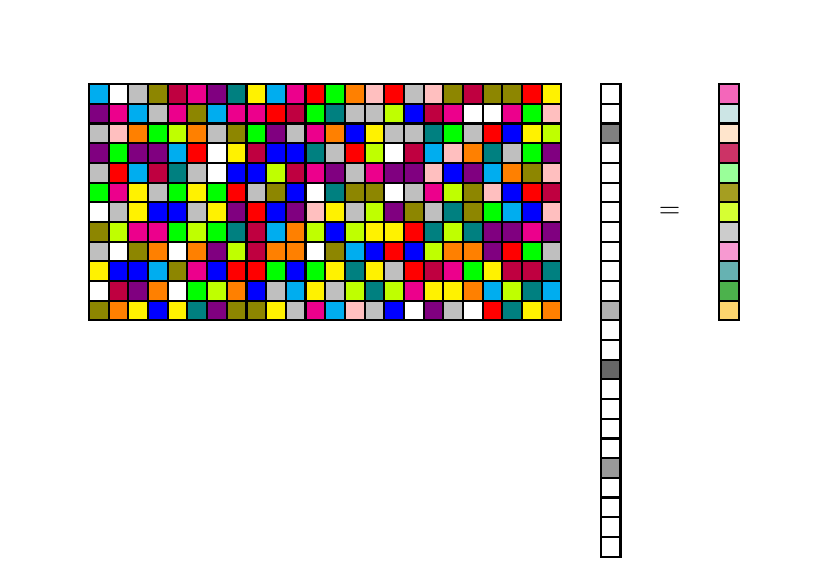
\begin{tikzpicture}
[draw=black, line width=0.75pt,
entry/.style={rectangle, draw, inner sep=0pt, minimum size=2.5mm},
symbol/.style={rectangle, draw, inner sep=0pt, minimum size=2.5mm}]

\node[entry, fill=olive] (x0y0) at (0.0,0.0) {};
\node[entry, fill=white] (x0y1) at (0.0,0.25) {};
\node[entry, fill=yellow] (x0y2) at (0.0,0.5) {};
\node[entry, fill=lightgray] (x0y3) at (0.0,0.75) {};
\node[entry, fill=olive] (x0y4) at (0.0,1.0) {};
\node[entry, fill=white] (x0y5) at (0.0,1.25) {};
\node[entry, fill=green] (x0y6) at (0.0,1.5) {};
\node[entry, fill=lightgray] (x0y7) at (0.0,1.75) {};
\node[entry, fill=violet] (x0y8) at (0.0,2.0) {};
\node[entry, fill=lightgray] (x0y9) at (0.0,2.25) {};
\node[entry, fill=violet] (x0y10) at (0.0,2.5) {};
\node[entry, fill=cyan] (x0y11) at (0.0,2.75) {};

\node[entry, fill=orange] (x1y0) at (0.25,0.0) {};
\node[entry, fill=purple] (x1y1) at (0.25,0.25) {};
\node[entry, fill=blue] (x1y2) at (0.25,0.5) {};
\node[entry, fill=white] (x1y3) at (0.25,0.75) {};
\node[entry, fill=lime] (x1y4) at (0.25,1.0) {};
\node[entry, fill=lightgray] (x1y5) at (0.25,1.25) {};
\node[entry, fill=magenta] (x1y6) at (0.25,1.5) {};
\node[entry, fill=red] (x1y7) at (0.25,1.75) {};
\node[entry, fill=green] (x1y8) at (0.25,2.0) {};
\node[entry, fill=pink] (x1y9) at (0.25,2.25) {};
\node[entry, fill=magenta] (x1y10) at (0.25,2.5) {};
\node[entry, fill=white] (x1y11) at (0.25,2.75) {};

\node[entry, fill=yellow] (x2y0) at (0.5,0.0) {};
\node[entry, fill=violet] (x2y1) at (0.5,0.25) {};
\node[entry, fill=blue] (x2y2) at (0.5,0.5) {};
\node[entry, fill=olive] (x2y3) at (0.5,0.75) {};
\node[entry, fill=magenta] (x2y4) at (0.5,1.0) {};
\node[entry, fill=yellow] (x2y5) at (0.5,1.25) {};
\node[entry, fill=yellow] (x2y6) at (0.5,1.5) {};
\node[entry, fill=cyan] (x2y7) at (0.5,1.75) {};
\node[entry, fill=violet] (x2y8) at (0.5,2.0) {};
\node[entry, fill=orange] (x2y9) at (0.5,2.25) {};
\node[entry, fill=cyan] (x2y10) at (0.5,2.5) {};
\node[entry, fill=lightgray] (x2y11) at (0.5,2.75) {};

\node[entry, fill=blue] (x3y0) at (0.75,0.0) {};
\node[entry, fill=orange] (x3y1) at (0.75,0.25) {};
\node[entry, fill=cyan] (x3y2) at (0.75,0.5) {};
\node[entry, fill=orange] (x3y3) at (0.75,0.75) {};
\node[entry, fill=magenta] (x3y4) at (0.75,1.0) {};
\node[entry, fill=blue] (x3y5) at (0.75,1.25) {};
\node[entry, fill=lightgray] (x3y6) at (0.75,1.5) {};
\node[entry, fill=purple] (x3y7) at (0.75,1.75) {};
\node[entry, fill=violet] (x3y8) at (0.75,2.0) {};
\node[entry, fill=green] (x3y9) at (0.75,2.25) {};
\node[entry, fill=lightgray] (x3y10) at (0.75,2.5) {};
\node[entry, fill=olive] (x3y11) at (0.75,2.75) {};

\node[entry, fill=yellow] (x4y0) at (1.0,0.0) {};
\node[entry, fill=white] (x4y1) at (1.0,0.25) {};
\node[entry, fill=olive] (x4y2) at (1.0,0.5) {};
\node[entry, fill=white] (x4y3) at (1.0,0.75) {};
\node[entry, fill=green] (x4y4) at (1.0,1.0) {};
\node[entry, fill=blue] (x4y5) at (1.0,1.25) {};
\node[entry, fill=green] (x4y6) at (1.0,1.5) {};
\node[entry, fill=teal] (x4y7) at (1.0,1.75) {};
\node[entry, fill=cyan] (x4y8) at (1.0,2.0) {};
\node[entry, fill=lime] (x4y9) at (1.0,2.25) {};
\node[entry, fill=magenta] (x4y10) at (1.0,2.5) {};
\node[entry, fill=purple] (x4y11) at (1.0,2.75) {};

\node[entry, fill=teal] (x5y0) at (1.25,0.0) {};
\node[entry, fill=green] (x5y1) at (1.25,0.25) {};
\node[entry, fill=magenta] (x5y2) at (1.25,0.5) {};
\node[entry, fill=orange] (x5y3) at (1.25,0.75) {};
\node[entry, fill=lime] (x5y4) at (1.25,1.0) {};
\node[entry, fill=lightgray] (x5y5) at (1.25,1.25) {};
\node[entry, fill=yellow] (x5y6) at (1.25,1.5) {};
\node[entry, fill=lightgray] (x5y7) at (1.25,1.75) {};
\node[entry, fill=red] (x5y8) at (1.25,2.0) {};
\node[entry, fill=orange] (x5y9) at (1.25,2.25) {};
\node[entry, fill=olive] (x5y10) at (1.25,2.5) {};
\node[entry, fill=magenta] (x5y11) at (1.25,2.75) {};

\node[entry, fill=violet] (x6y0) at (1.5,0.0) {};
\node[entry, fill=lime] (x6y1) at (1.5,0.25) {};
\node[entry, fill=blue] (x6y2) at (1.5,0.5) {};
\node[entry, fill=violet] (x6y3) at (1.5,0.75) {};
\node[entry, fill=green] (x6y4) at (1.5,1.0) {};
\node[entry, fill=yellow] (x6y5) at (1.5,1.25) {};
\node[entry, fill=green] (x6y6) at (1.5,1.5) {};
\node[entry, fill=white] (x6y7) at (1.5,1.75) {};
\node[entry, fill=white] (x6y8) at (1.5,2.0) {};
\node[entry, fill=lightgray] (x6y9) at (1.5,2.25) {};
\node[entry, fill=cyan] (x6y10) at (1.5,2.5) {};
\node[entry, fill=violet] (x6y11) at (1.5,2.75) {};

\node[entry, fill=olive] (x7y0) at (1.75,0.0) {};
\node[entry, fill=orange] (x7y1) at (1.75,0.25) {};
\node[entry, fill=red] (x7y2) at (1.75,0.5) {};
\node[entry, fill=lime] (x7y3) at (1.75,0.75) {};
\node[entry, fill=teal] (x7y4) at (1.75,1.0) {};
\node[entry, fill=violet] (x7y5) at (1.75,1.25) {};
\node[entry, fill=red] (x7y6) at (1.75,1.5) {};
\node[entry, fill=blue] (x7y7) at (1.75,1.75) {};
\node[entry, fill=yellow] (x7y8) at (1.75,2.0) {};
\node[entry, fill=olive] (x7y9) at (1.75,2.25) {};
\node[entry, fill=magenta] (x7y10) at (1.75,2.5) {};
\node[entry, fill=teal] (x7y11) at (1.75,2.75) {};

\node[entry, fill=olive] (x8y0) at (2.0,0.0) {};
\node[entry, fill=blue] (x8y1) at (2.0,0.25) {};
\node[entry, fill=red] (x8y2) at (2.0,0.5) {};
\node[entry, fill=purple] (x8y3) at (2.0,0.75) {};
\node[entry, fill=purple] (x8y4) at (2.0,1.0) {};
\node[entry, fill=red] (x8y5) at (2.0,1.25) {};
\node[entry, fill=lightgray] (x8y6) at (2.0,1.5) {};
\node[entry, fill=blue] (x8y7) at (2.0,1.75) {};
\node[entry, fill=purple] (x8y8) at (2.0,2.0) {};
\node[entry, fill=green] (x8y9) at (2.0,2.25) {};
\node[entry, fill=magenta] (x8y10) at (2.0,2.5) {};
\node[entry, fill=yellow] (x8y11) at (2.0,2.75) {};

\node[entry, fill=yellow] (x9y0) at (2.25,0.0) {};
\node[entry, fill=lightgray] (x9y1) at (2.25,0.25) {};
\node[entry, fill=green] (x9y2) at (2.25,0.5) {};
\node[entry, fill=orange] (x9y3) at (2.25,0.75) {};
\node[entry, fill=cyan] (x9y4) at (2.25,1.0) {};
\node[entry, fill=blue] (x9y5) at (2.25,1.25) {};
\node[entry, fill=olive] (x9y6) at (2.25,1.5) {};
\node[entry, fill=lime] (x9y7) at (2.25,1.75) {};
\node[entry, fill=blue] (x9y8) at (2.25,2.0) {};
\node[entry, fill=violet] (x9y9) at (2.25,2.25) {};
\node[entry, fill=red] (x9y10) at (2.25,2.5) {};
\node[entry, fill=cyan] (x9y11) at (2.25,2.75) {};

\node[entry, fill=lightgray] (x10y0) at (2.5,0.0) {};
\node[entry, fill=cyan] (x10y1) at (2.5,0.25) {};
\node[entry, fill=blue] (x10y2) at (2.5,0.5) {};
\node[entry, fill=orange] (x10y3) at (2.5,0.75) {};
\node[entry, fill=orange] (x10y4) at (2.5,1.0) {};
\node[entry, fill=violet] (x10y5) at (2.5,1.25) {};
\node[entry, fill=blue] (x10y6) at (2.5,1.5) {};
\node[entry, fill=purple] (x10y7) at (2.5,1.75) {};
\node[entry, fill=blue] (x10y8) at (2.5,2.0) {};
\node[entry, fill=lightgray] (x10y9) at (2.5,2.25) {};
\node[entry, fill=purple] (x10y10) at (2.5,2.5) {};
\node[entry, fill=magenta] (x10y11) at (2.5,2.75) {};

\node[entry, fill=magenta] (x11y0) at (2.75,0.0) {};
\node[entry, fill=yellow] (x11y1) at (2.75,0.25) {};
\node[entry, fill=green] (x11y2) at (2.75,0.5) {};
\node[entry, fill=white] (x11y3) at (2.75,0.75) {};
\node[entry, fill=lime] (x11y4) at (2.75,1.0) {};
\node[entry, fill=pink] (x11y5) at (2.75,1.25) {};
\node[entry, fill=white] (x11y6) at (2.75,1.5) {};
\node[entry, fill=magenta] (x11y7) at (2.75,1.75) {};
\node[entry, fill=teal] (x11y8) at (2.75,2.0) {};
\node[entry, fill=magenta] (x11y9) at (2.75,2.25) {};
\node[entry, fill=green] (x11y10) at (2.75,2.5) {};
\node[entry, fill=red] (x11y11) at (2.75,2.75) {};

\node[entry, fill=cyan] (x12y0) at (3.0,0.0) {};
\node[entry, fill=lightgray] (x12y1) at (3.0,0.25) {};
\node[entry, fill=yellow] (x12y2) at (3.0,0.5) {};
\node[entry, fill=olive] (x12y3) at (3.0,0.75) {};
\node[entry, fill=blue] (x12y4) at (3.0,1.0) {};
\node[entry, fill=yellow] (x12y5) at (3.0,1.25) {};
\node[entry, fill=teal] (x12y6) at (3.0,1.5) {};
\node[entry, fill=violet] (x12y7) at (3.0,1.75) {};
\node[entry, fill=lightgray] (x12y8) at (3.0,2.0) {};
\node[entry, fill=orange] (x12y9) at (3.0,2.25) {};
\node[entry, fill=teal] (x12y10) at (3.0,2.5) {};
\node[entry, fill=green] (x12y11) at (3.0,2.75) {};

\node[entry, fill=pink] (x13y0) at (3.25,0.0) {};
\node[entry, fill=lime] (x13y1) at (3.25,0.25) {};
\node[entry, fill=teal] (x13y2) at (3.25,0.5) {};
\node[entry, fill=cyan] (x13y3) at (3.25,0.75) {};
\node[entry, fill=lime] (x13y4) at (3.25,1.0) {};
\node[entry, fill=lightgray] (x13y5) at (3.25,1.25) {};
\node[entry, fill=olive] (x13y6) at (3.25,1.5) {};
\node[entry, fill=lightgray] (x13y7) at (3.25,1.75) {};
\node[entry, fill=red] (x13y8) at (3.25,2.0) {};
\node[entry, fill=blue] (x13y9) at (3.25,2.25) {};
\node[entry, fill=lightgray] (x13y10) at (3.25,2.5) {};
\node[entry, fill=orange] (x13y11) at (3.25,2.75) {};

\node[entry, fill=lightgray] (x14y0) at (3.5,0.0) {};
\node[entry, fill=teal] (x14y1) at (3.5,0.25) {};
\node[entry, fill=yellow] (x14y2) at (3.5,0.5) {};
\node[entry, fill=blue] (x14y3) at (3.5,0.75) {};
\node[entry, fill=yellow] (x14y4) at (3.5,1.0) {};
\node[entry, fill=lime] (x14y5) at (3.5,1.25) {};
\node[entry, fill=olive] (x14y6) at (3.5,1.5) {};
\node[entry, fill=magenta] (x14y7) at (3.5,1.75) {};
\node[entry, fill=lime] (x14y8) at (3.5,2.0) {};
\node[entry, fill=yellow] (x14y9) at (3.5,2.25) {};
\node[entry, fill=lightgray] (x14y10) at (3.5,2.5) {};
\node[entry, fill=pink] (x14y11) at (3.5,2.75) {};

\node[entry, fill=blue] (x15y0) at (3.75,0.0) {};
\node[entry, fill=lime] (x15y1) at (3.75,0.25) {};
\node[entry, fill=lightgray] (x15y2) at (3.75,0.5) {};
\node[entry, fill=red] (x15y3) at (3.75,0.75) {};
\node[entry, fill=yellow] (x15y4) at (3.75,1.0) {};
\node[entry, fill=violet] (x15y5) at (3.75,1.25) {};
\node[entry, fill=white] (x15y6) at (3.75,1.5) {};
\node[entry, fill=violet] (x15y7) at (3.75,1.75) {};
\node[entry, fill=white] (x15y8) at (3.75,2.0) {};
\node[entry, fill=lightgray] (x15y9) at (3.75,2.25) {};
\node[entry, fill=lime] (x15y10) at (3.75,2.5) {};
\node[entry, fill=red] (x15y11) at (3.75,2.75) {};

\node[entry, fill=white] (x16y0) at (4.0,0.0) {};
\node[entry, fill=magenta] (x16y1) at (4.0,0.25) {};
\node[entry, fill=red] (x16y2) at (4.0,0.5) {};
\node[entry, fill=blue] (x16y3) at (4.0,0.75) {};
\node[entry, fill=red] (x16y4) at (4.0,1.0) {};
\node[entry, fill=olive] (x16y5) at (4.0,1.25) {};
\node[entry, fill=lightgray] (x16y6) at (4.0,1.5) {};
\node[entry, fill=violet] (x16y7) at (4.0,1.75) {};
\node[entry, fill=purple] (x16y8) at (4.0,2.0) {};
\node[entry, fill=lightgray] (x16y9) at (4.0,2.25) {};
\node[entry, fill=blue] (x16y10) at (4.0,2.5) {};
\node[entry, fill=lightgray] (x16y11) at (4.0,2.75) {};

\node[entry, fill=violet] (x17y0) at (4.25,0.0) {};
\node[entry, fill=yellow] (x17y1) at (4.25,0.25) {};
\node[entry, fill=purple] (x17y2) at (4.25,0.5) {};
\node[entry, fill=lime] (x17y3) at (4.25,0.75) {};
\node[entry, fill=teal] (x17y4) at (4.25,1.0) {};
\node[entry, fill=lightgray] (x17y5) at (4.25,1.25) {};
\node[entry, fill=magenta] (x17y6) at (4.25,1.5) {};
\node[entry, fill=pink] (x17y7) at (4.25,1.75) {};
\node[entry, fill=cyan] (x17y8) at (4.25,2.0) {};
\node[entry, fill=teal] (x17y9) at (4.25,2.25) {};
\node[entry, fill=purple] (x17y10) at (4.25,2.5) {};
\node[entry, fill=pink] (x17y11) at (4.25,2.75) {};

\node[entry, fill=lightgray] (x18y0) at (4.5,0.0) {};
\node[entry, fill=yellow] (x18y1) at (4.5,0.25) {};
\node[entry, fill=magenta] (x18y2) at (4.5,0.5) {};
\node[entry, fill=orange] (x18y3) at (4.5,0.75) {};
\node[entry, fill=lime] (x18y4) at (4.5,1.0) {};
\node[entry, fill=teal] (x18y5) at (4.5,1.25) {};
\node[entry, fill=lime] (x18y6) at (4.5,1.5) {};
\node[entry, fill=blue] (x18y7) at (4.5,1.75) {};
\node[entry, fill=pink] (x18y8) at (4.5,2.0) {};
\node[entry, fill=green] (x18y9) at (4.5,2.25) {};
\node[entry, fill=magenta] (x18y10) at (4.5,2.5) {};
\node[entry, fill=olive] (x18y11) at (4.5,2.75) {};

\node[entry, fill=white] (x19y0) at (4.75,0.0) {};
\node[entry, fill=orange] (x19y1) at (4.75,0.25) {};
\node[entry, fill=green] (x19y2) at (4.75,0.5) {};
\node[entry, fill=orange] (x19y3) at (4.75,0.75) {};
\node[entry, fill=teal] (x19y4) at (4.75,1.0) {};
\node[entry, fill=olive] (x19y5) at (4.75,1.25) {};
\node[entry, fill=olive] (x19y6) at (4.75,1.5) {};
\node[entry, fill=violet] (x19y7) at (4.75,1.75) {};
\node[entry, fill=orange] (x19y8) at (4.75,2.0) {};
\node[entry, fill=lightgray] (x19y9) at (4.75,2.25) {};
\node[entry, fill=white] (x19y10) at (4.75,2.5) {};
\node[entry, fill=purple] (x19y11) at (4.75,2.75) {};

\node[entry, fill=red] (x20y0) at (5.0,0.0) {};
\node[entry, fill=cyan] (x20y1) at (5.0,0.25) {};
\node[entry, fill=yellow] (x20y2) at (5.0,0.5) {};
\node[entry, fill=violet] (x20y3) at (5.0,0.75) {};
\node[entry, fill=violet] (x20y4) at (5.0,1.0) {};
\node[entry, fill=green] (x20y5) at (5.0,1.25) {};
\node[entry, fill=pink] (x20y6) at (5.0,1.5) {};
\node[entry, fill=cyan] (x20y7) at (5.0,1.75) {};
\node[entry, fill=teal] (x20y8) at (5.0,2.0) {};
\node[entry, fill=red] (x20y9) at (5.0,2.25) {};
\node[entry, fill=white] (x20y10) at (5.0,2.5) {};
\node[entry, fill=olive] (x20y11) at (5.0,2.75) {};

\node[entry, fill=teal] (x21y0) at (5.25,0.0) {};
\node[entry, fill=lime] (x21y1) at (5.25,0.25) {};
\node[entry, fill=purple] (x21y2) at (5.25,0.5) {};
\node[entry, fill=red] (x21y3) at (5.25,0.75) {};
\node[entry, fill=violet] (x21y4) at (5.25,1.0) {};
\node[entry, fill=cyan] (x21y5) at (5.25,1.25) {};
\node[entry, fill=blue] (x21y6) at (5.25,1.5) {};
\node[entry, fill=orange] (x21y7) at (5.25,1.75) {};
\node[entry, fill=lightgray] (x21y8) at (5.25,2.0) {};
\node[entry, fill=blue] (x21y9) at (5.25,2.25) {};
\node[entry, fill=magenta] (x21y10) at (5.25,2.5) {};
\node[entry, fill=olive] (x21y11) at (5.25,2.75) {};

\node[entry, fill=yellow] (x22y0) at (5.5,0.0) {};
\node[entry, fill=teal] (x22y1) at (5.5,0.25) {};
\node[entry, fill=purple] (x22y2) at (5.5,0.5) {};
\node[entry, fill=green] (x22y3) at (5.5,0.75) {};
\node[entry, fill=magenta] (x22y4) at (5.5,1.0) {};
\node[entry, fill=blue] (x22y5) at (5.5,1.25) {};
\node[entry, fill=red] (x22y6) at (5.5,1.5) {};
\node[entry, fill=olive] (x22y7) at (5.5,1.75) {};
\node[entry, fill=green] (x22y8) at (5.5,2.0) {};
\node[entry, fill=yellow] (x22y9) at (5.5,2.25) {};
\node[entry, fill=green] (x22y10) at (5.5,2.5) {};
\node[entry, fill=red] (x22y11) at (5.5,2.75) {};

\node[entry, fill=orange] (x23y0) at (5.75,0.0) {};
\node[entry, fill=cyan] (x23y1) at (5.75,0.25) {};
\node[entry, fill=teal] (x23y2) at (5.75,0.5) {};
\node[entry, fill=lightgray] (x23y3) at (5.75,0.75) {};
\node[entry, fill=violet] (x23y4) at (5.75,1.0) {};
\node[entry, fill=pink] (x23y5) at (5.75,1.25) {};
\node[entry, fill=purple] (x23y6) at (5.75,1.5) {};
\node[entry, fill=pink] (x23y7) at (5.75,1.75) {};
\node[entry, fill=violet] (x23y8) at (5.75,2.0) {};
\node[entry, fill=lime] (x23y9) at (5.75,2.25) {};
\node[entry, fill=pink] (x23y10) at (5.75,2.5) {};
\node[entry, fill=yellow] (x23y11) at (5.75,2.75) {};

\node[symbol] (s01) at (6.5,-3.00) {};
\node[symbol] (s02) at (6.5,-2.75) {};
\node[symbol] (s03) at (6.5,-2.50) {};
\node[symbol] (s04) at (6.5,-2.25) {};
\node[symbol,fill=black!40] (s05) at (6.5,-2.00) {};
\node[symbol] (s06) at (6.5,-1.75) {};
\node[symbol] (s07) at (6.5,-1.50) {};
\node[symbol] (s08) at (6.5,-1.25) {};
\node[symbol] (s09) at (6.5,-1.00) {};
\node[symbol,fill=black!60] (s10) at (6.5,-0.75) {};
\node[symbol] (s11) at (6.5,-0.50) {};
\node[symbol] (s12) at (6.5,-0.25) {};
\node[symbol,fill=black!30] (s13) at (6.5,0) {};
\node[symbol] (s14) at (6.5,0.25) {};
\node[symbol] (s15) at (6.5,0.50) {};
\node[symbol] (s16) at (6.5,0.75) {};
\node[symbol] (s17) at (6.5,1.00) {};
\node[symbol] (s18) at (6.5,1.25) {};
\node[symbol] (s19) at (6.5,1.50) {};
\node[symbol] (s20) at (6.5,1.75) {};
\node[symbol] (s21) at (6.5,2.00) {};
\node[symbol,fill=black!50] (s22) at (6.5,2.25) {};
\node[symbol] (s23) at (6.5,2.50) {};
\node[symbol] (s24) at (6.5,2.75) {};

\node (equal) at (7.25,1.25) {$=$};

\node[entry, fill=yellow!40!pink] (o0) at (8,0.0) {};
\node[entry, fill=gray!60!green] (o1) at (8,0.25) {};
\node[entry, fill=teal!60] (o2) at (8,0.5) {};
\node[entry, fill=magenta!40] (o3) at (8,0.75) {};
\node[entry, fill=gray!40] (o4) at (8,1.0) {};
\node[entry, fill=green!20!yellow!80] (o5) at (8,1.25) {};
\node[entry, fill=olive!80] (o6) at (8,1.5) {};
\node[entry, fill=green!40] (o7) at (8,1.75) {};
\node[entry, fill=purple!80] (o8) at (8,2.0) {};
\node[entry, fill=orange!20] (o9) at (8,2.25) {};
\node[entry, fill=teal!20] (o10) at (8,2.5) {};
\node[entry, fill=magenta!60] (o11) at (8,2.75) {};

\draw[|-|,opacity=0] (-0.125, 3.125) to node[above] {\small Number of columns} (5.875, 3.125);
\draw[|-|,opacity=0] (-0.375, -0.125) to node[above,rotate=90] {\small Number of samples} (-0.375, 2.875);
\draw[|-|,opacity=0] (6.875, -3.125) to node[above,rotate=-90] {\small Number of non-zero entries} (6.875, 2.875);
\node[opacity=0] (framework) at (2.875,-0.5) {Sensing matrix $\boldsymbol{\Phi}$};
\node[rotate=-90,opacity=0] (vector) at (7,-0.75) {Sparse vector $\mathbf{s}$};
\node[rotate=-90,opacity=0] (observation) at (8.5,1.5) {Observation $\mathbf{y}$};
\end{tikzpicture}
 \end{center}
\end{frame}

% % % % % % % % % % % % % % % % % % % %

\begin{frame} \frametitle{Compressed Sensing -- Brief Overview}
\begin{center} \input{Figures-CS/compressivesampling0} \end{center}
\end{frame}

% % % % % % % % % % % % % % % % % % % %

\begin{frame} \frametitle{Compressed Sensing -- Brief Overview}
\begin{center} \input{Figures-CS/compressivesampling0a} \end{center}
\end{frame}

% % % % % % % % % % % % % % % % % % % %

\begin{frame} \frametitle{Compressed Sensing -- Brief Overview}
\begin{center} \input{Figures-CS/compressivesampling0b} \end{center}
\end{frame}

% % % % % % % % % % % % % % % % % % % %

\begin{frame} \frametitle{Compressed Sensing -- Brief Overview}
\begin{center} \input{Figures-CS/compressivesampling0c} \end{center}
\end{frame}

% % % % % % % % % % % % % % % % % % % %

%\begin{frame} \frametitle{Compressed Sensing -- Brief Overview}
%\begin{center} \input{Figures-CS/compressivesampling0b} \end{center}
%\end{frame}

% % % % % % % % % % % % % % % % % % % %

\begin{frame} \frametitle{Compressed Sensing -- Brief Overview}
\begin{center} \input{Figures-CS/compressivesampling1} \end{center}
\end{frame}

% % % % % % % % % % % % % % % % % % % %

\begin{frame} \frametitle{Compressed Sensing -- Brief Overview}
\begin{center} \input{Figures-CS/compressivesampling1a} \end{center}
\end{frame}

% % % % % % % % % % % % % % % % % % % %

\begin{frame} \frametitle{Compressed Sensing -- Brief Overview}
\begin{center} \input{Figures-CS/compressivesampling1b} \end{center}
\end{frame}

% % % % % % % % % % % % % % % % % % % %

\begin{frame} \frametitle{Compressed Sensing -- Brief Overview}
\begin{center} \input{Figures-CS/compressivesampling1c} \end{center}
\end{frame}

% % % % % % % % % % % % % % % % % % % %

\begin{frame}
\frametitle{Compressed Sensing -- Basis Pursuit -- LASSO}
% % % % %
\hfill
\scalebox{0.5}{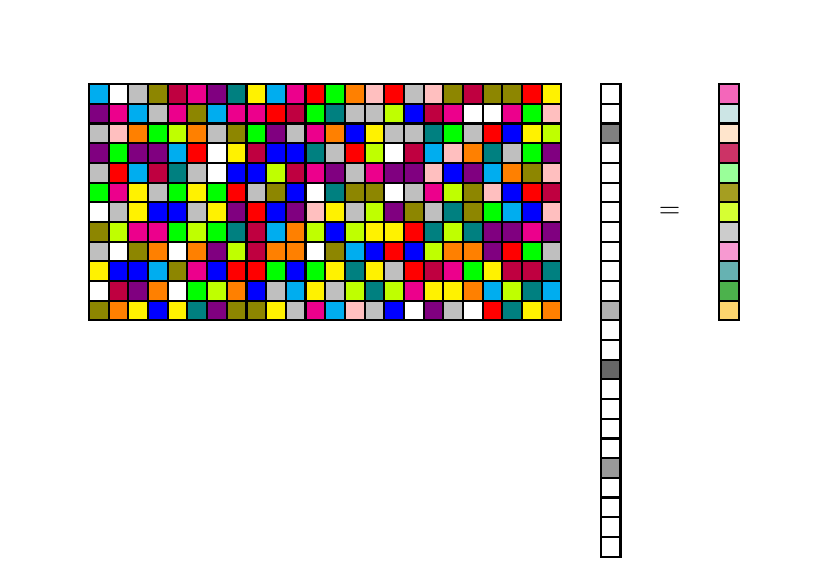
\begin{tikzpicture}
[draw=black, line width=0.75pt,
entry/.style={rectangle, draw, inner sep=0pt, minimum size=2.5mm},
symbol/.style={rectangle, draw, inner sep=0pt, minimum size=2.5mm}]

\node[entry, fill=olive] (x0y0) at (0.0,0.0) {};
\node[entry, fill=white] (x0y1) at (0.0,0.25) {};
\node[entry, fill=yellow] (x0y2) at (0.0,0.5) {};
\node[entry, fill=lightgray] (x0y3) at (0.0,0.75) {};
\node[entry, fill=olive] (x0y4) at (0.0,1.0) {};
\node[entry, fill=white] (x0y5) at (0.0,1.25) {};
\node[entry, fill=green] (x0y6) at (0.0,1.5) {};
\node[entry, fill=lightgray] (x0y7) at (0.0,1.75) {};
\node[entry, fill=violet] (x0y8) at (0.0,2.0) {};
\node[entry, fill=lightgray] (x0y9) at (0.0,2.25) {};
\node[entry, fill=violet] (x0y10) at (0.0,2.5) {};
\node[entry, fill=cyan] (x0y11) at (0.0,2.75) {};

\node[entry, fill=orange] (x1y0) at (0.25,0.0) {};
\node[entry, fill=purple] (x1y1) at (0.25,0.25) {};
\node[entry, fill=blue] (x1y2) at (0.25,0.5) {};
\node[entry, fill=white] (x1y3) at (0.25,0.75) {};
\node[entry, fill=lime] (x1y4) at (0.25,1.0) {};
\node[entry, fill=lightgray] (x1y5) at (0.25,1.25) {};
\node[entry, fill=magenta] (x1y6) at (0.25,1.5) {};
\node[entry, fill=red] (x1y7) at (0.25,1.75) {};
\node[entry, fill=green] (x1y8) at (0.25,2.0) {};
\node[entry, fill=pink] (x1y9) at (0.25,2.25) {};
\node[entry, fill=magenta] (x1y10) at (0.25,2.5) {};
\node[entry, fill=white] (x1y11) at (0.25,2.75) {};

\node[entry, fill=yellow] (x2y0) at (0.5,0.0) {};
\node[entry, fill=violet] (x2y1) at (0.5,0.25) {};
\node[entry, fill=blue] (x2y2) at (0.5,0.5) {};
\node[entry, fill=olive] (x2y3) at (0.5,0.75) {};
\node[entry, fill=magenta] (x2y4) at (0.5,1.0) {};
\node[entry, fill=yellow] (x2y5) at (0.5,1.25) {};
\node[entry, fill=yellow] (x2y6) at (0.5,1.5) {};
\node[entry, fill=cyan] (x2y7) at (0.5,1.75) {};
\node[entry, fill=violet] (x2y8) at (0.5,2.0) {};
\node[entry, fill=orange] (x2y9) at (0.5,2.25) {};
\node[entry, fill=cyan] (x2y10) at (0.5,2.5) {};
\node[entry, fill=lightgray] (x2y11) at (0.5,2.75) {};

\node[entry, fill=blue] (x3y0) at (0.75,0.0) {};
\node[entry, fill=orange] (x3y1) at (0.75,0.25) {};
\node[entry, fill=cyan] (x3y2) at (0.75,0.5) {};
\node[entry, fill=orange] (x3y3) at (0.75,0.75) {};
\node[entry, fill=magenta] (x3y4) at (0.75,1.0) {};
\node[entry, fill=blue] (x3y5) at (0.75,1.25) {};
\node[entry, fill=lightgray] (x3y6) at (0.75,1.5) {};
\node[entry, fill=purple] (x3y7) at (0.75,1.75) {};
\node[entry, fill=violet] (x3y8) at (0.75,2.0) {};
\node[entry, fill=green] (x3y9) at (0.75,2.25) {};
\node[entry, fill=lightgray] (x3y10) at (0.75,2.5) {};
\node[entry, fill=olive] (x3y11) at (0.75,2.75) {};

\node[entry, fill=yellow] (x4y0) at (1.0,0.0) {};
\node[entry, fill=white] (x4y1) at (1.0,0.25) {};
\node[entry, fill=olive] (x4y2) at (1.0,0.5) {};
\node[entry, fill=white] (x4y3) at (1.0,0.75) {};
\node[entry, fill=green] (x4y4) at (1.0,1.0) {};
\node[entry, fill=blue] (x4y5) at (1.0,1.25) {};
\node[entry, fill=green] (x4y6) at (1.0,1.5) {};
\node[entry, fill=teal] (x4y7) at (1.0,1.75) {};
\node[entry, fill=cyan] (x4y8) at (1.0,2.0) {};
\node[entry, fill=lime] (x4y9) at (1.0,2.25) {};
\node[entry, fill=magenta] (x4y10) at (1.0,2.5) {};
\node[entry, fill=purple] (x4y11) at (1.0,2.75) {};

\node[entry, fill=teal] (x5y0) at (1.25,0.0) {};
\node[entry, fill=green] (x5y1) at (1.25,0.25) {};
\node[entry, fill=magenta] (x5y2) at (1.25,0.5) {};
\node[entry, fill=orange] (x5y3) at (1.25,0.75) {};
\node[entry, fill=lime] (x5y4) at (1.25,1.0) {};
\node[entry, fill=lightgray] (x5y5) at (1.25,1.25) {};
\node[entry, fill=yellow] (x5y6) at (1.25,1.5) {};
\node[entry, fill=lightgray] (x5y7) at (1.25,1.75) {};
\node[entry, fill=red] (x5y8) at (1.25,2.0) {};
\node[entry, fill=orange] (x5y9) at (1.25,2.25) {};
\node[entry, fill=olive] (x5y10) at (1.25,2.5) {};
\node[entry, fill=magenta] (x5y11) at (1.25,2.75) {};

\node[entry, fill=violet] (x6y0) at (1.5,0.0) {};
\node[entry, fill=lime] (x6y1) at (1.5,0.25) {};
\node[entry, fill=blue] (x6y2) at (1.5,0.5) {};
\node[entry, fill=violet] (x6y3) at (1.5,0.75) {};
\node[entry, fill=green] (x6y4) at (1.5,1.0) {};
\node[entry, fill=yellow] (x6y5) at (1.5,1.25) {};
\node[entry, fill=green] (x6y6) at (1.5,1.5) {};
\node[entry, fill=white] (x6y7) at (1.5,1.75) {};
\node[entry, fill=white] (x6y8) at (1.5,2.0) {};
\node[entry, fill=lightgray] (x6y9) at (1.5,2.25) {};
\node[entry, fill=cyan] (x6y10) at (1.5,2.5) {};
\node[entry, fill=violet] (x6y11) at (1.5,2.75) {};

\node[entry, fill=olive] (x7y0) at (1.75,0.0) {};
\node[entry, fill=orange] (x7y1) at (1.75,0.25) {};
\node[entry, fill=red] (x7y2) at (1.75,0.5) {};
\node[entry, fill=lime] (x7y3) at (1.75,0.75) {};
\node[entry, fill=teal] (x7y4) at (1.75,1.0) {};
\node[entry, fill=violet] (x7y5) at (1.75,1.25) {};
\node[entry, fill=red] (x7y6) at (1.75,1.5) {};
\node[entry, fill=blue] (x7y7) at (1.75,1.75) {};
\node[entry, fill=yellow] (x7y8) at (1.75,2.0) {};
\node[entry, fill=olive] (x7y9) at (1.75,2.25) {};
\node[entry, fill=magenta] (x7y10) at (1.75,2.5) {};
\node[entry, fill=teal] (x7y11) at (1.75,2.75) {};

\node[entry, fill=olive] (x8y0) at (2.0,0.0) {};
\node[entry, fill=blue] (x8y1) at (2.0,0.25) {};
\node[entry, fill=red] (x8y2) at (2.0,0.5) {};
\node[entry, fill=purple] (x8y3) at (2.0,0.75) {};
\node[entry, fill=purple] (x8y4) at (2.0,1.0) {};
\node[entry, fill=red] (x8y5) at (2.0,1.25) {};
\node[entry, fill=lightgray] (x8y6) at (2.0,1.5) {};
\node[entry, fill=blue] (x8y7) at (2.0,1.75) {};
\node[entry, fill=purple] (x8y8) at (2.0,2.0) {};
\node[entry, fill=green] (x8y9) at (2.0,2.25) {};
\node[entry, fill=magenta] (x8y10) at (2.0,2.5) {};
\node[entry, fill=yellow] (x8y11) at (2.0,2.75) {};

\node[entry, fill=yellow] (x9y0) at (2.25,0.0) {};
\node[entry, fill=lightgray] (x9y1) at (2.25,0.25) {};
\node[entry, fill=green] (x9y2) at (2.25,0.5) {};
\node[entry, fill=orange] (x9y3) at (2.25,0.75) {};
\node[entry, fill=cyan] (x9y4) at (2.25,1.0) {};
\node[entry, fill=blue] (x9y5) at (2.25,1.25) {};
\node[entry, fill=olive] (x9y6) at (2.25,1.5) {};
\node[entry, fill=lime] (x9y7) at (2.25,1.75) {};
\node[entry, fill=blue] (x9y8) at (2.25,2.0) {};
\node[entry, fill=violet] (x9y9) at (2.25,2.25) {};
\node[entry, fill=red] (x9y10) at (2.25,2.5) {};
\node[entry, fill=cyan] (x9y11) at (2.25,2.75) {};

\node[entry, fill=lightgray] (x10y0) at (2.5,0.0) {};
\node[entry, fill=cyan] (x10y1) at (2.5,0.25) {};
\node[entry, fill=blue] (x10y2) at (2.5,0.5) {};
\node[entry, fill=orange] (x10y3) at (2.5,0.75) {};
\node[entry, fill=orange] (x10y4) at (2.5,1.0) {};
\node[entry, fill=violet] (x10y5) at (2.5,1.25) {};
\node[entry, fill=blue] (x10y6) at (2.5,1.5) {};
\node[entry, fill=purple] (x10y7) at (2.5,1.75) {};
\node[entry, fill=blue] (x10y8) at (2.5,2.0) {};
\node[entry, fill=lightgray] (x10y9) at (2.5,2.25) {};
\node[entry, fill=purple] (x10y10) at (2.5,2.5) {};
\node[entry, fill=magenta] (x10y11) at (2.5,2.75) {};

\node[entry, fill=magenta] (x11y0) at (2.75,0.0) {};
\node[entry, fill=yellow] (x11y1) at (2.75,0.25) {};
\node[entry, fill=green] (x11y2) at (2.75,0.5) {};
\node[entry, fill=white] (x11y3) at (2.75,0.75) {};
\node[entry, fill=lime] (x11y4) at (2.75,1.0) {};
\node[entry, fill=pink] (x11y5) at (2.75,1.25) {};
\node[entry, fill=white] (x11y6) at (2.75,1.5) {};
\node[entry, fill=magenta] (x11y7) at (2.75,1.75) {};
\node[entry, fill=teal] (x11y8) at (2.75,2.0) {};
\node[entry, fill=magenta] (x11y9) at (2.75,2.25) {};
\node[entry, fill=green] (x11y10) at (2.75,2.5) {};
\node[entry, fill=red] (x11y11) at (2.75,2.75) {};

\node[entry, fill=cyan] (x12y0) at (3.0,0.0) {};
\node[entry, fill=lightgray] (x12y1) at (3.0,0.25) {};
\node[entry, fill=yellow] (x12y2) at (3.0,0.5) {};
\node[entry, fill=olive] (x12y3) at (3.0,0.75) {};
\node[entry, fill=blue] (x12y4) at (3.0,1.0) {};
\node[entry, fill=yellow] (x12y5) at (3.0,1.25) {};
\node[entry, fill=teal] (x12y6) at (3.0,1.5) {};
\node[entry, fill=violet] (x12y7) at (3.0,1.75) {};
\node[entry, fill=lightgray] (x12y8) at (3.0,2.0) {};
\node[entry, fill=orange] (x12y9) at (3.0,2.25) {};
\node[entry, fill=teal] (x12y10) at (3.0,2.5) {};
\node[entry, fill=green] (x12y11) at (3.0,2.75) {};

\node[entry, fill=pink] (x13y0) at (3.25,0.0) {};
\node[entry, fill=lime] (x13y1) at (3.25,0.25) {};
\node[entry, fill=teal] (x13y2) at (3.25,0.5) {};
\node[entry, fill=cyan] (x13y3) at (3.25,0.75) {};
\node[entry, fill=lime] (x13y4) at (3.25,1.0) {};
\node[entry, fill=lightgray] (x13y5) at (3.25,1.25) {};
\node[entry, fill=olive] (x13y6) at (3.25,1.5) {};
\node[entry, fill=lightgray] (x13y7) at (3.25,1.75) {};
\node[entry, fill=red] (x13y8) at (3.25,2.0) {};
\node[entry, fill=blue] (x13y9) at (3.25,2.25) {};
\node[entry, fill=lightgray] (x13y10) at (3.25,2.5) {};
\node[entry, fill=orange] (x13y11) at (3.25,2.75) {};

\node[entry, fill=lightgray] (x14y0) at (3.5,0.0) {};
\node[entry, fill=teal] (x14y1) at (3.5,0.25) {};
\node[entry, fill=yellow] (x14y2) at (3.5,0.5) {};
\node[entry, fill=blue] (x14y3) at (3.5,0.75) {};
\node[entry, fill=yellow] (x14y4) at (3.5,1.0) {};
\node[entry, fill=lime] (x14y5) at (3.5,1.25) {};
\node[entry, fill=olive] (x14y6) at (3.5,1.5) {};
\node[entry, fill=magenta] (x14y7) at (3.5,1.75) {};
\node[entry, fill=lime] (x14y8) at (3.5,2.0) {};
\node[entry, fill=yellow] (x14y9) at (3.5,2.25) {};
\node[entry, fill=lightgray] (x14y10) at (3.5,2.5) {};
\node[entry, fill=pink] (x14y11) at (3.5,2.75) {};

\node[entry, fill=blue] (x15y0) at (3.75,0.0) {};
\node[entry, fill=lime] (x15y1) at (3.75,0.25) {};
\node[entry, fill=lightgray] (x15y2) at (3.75,0.5) {};
\node[entry, fill=red] (x15y3) at (3.75,0.75) {};
\node[entry, fill=yellow] (x15y4) at (3.75,1.0) {};
\node[entry, fill=violet] (x15y5) at (3.75,1.25) {};
\node[entry, fill=white] (x15y6) at (3.75,1.5) {};
\node[entry, fill=violet] (x15y7) at (3.75,1.75) {};
\node[entry, fill=white] (x15y8) at (3.75,2.0) {};
\node[entry, fill=lightgray] (x15y9) at (3.75,2.25) {};
\node[entry, fill=lime] (x15y10) at (3.75,2.5) {};
\node[entry, fill=red] (x15y11) at (3.75,2.75) {};

\node[entry, fill=white] (x16y0) at (4.0,0.0) {};
\node[entry, fill=magenta] (x16y1) at (4.0,0.25) {};
\node[entry, fill=red] (x16y2) at (4.0,0.5) {};
\node[entry, fill=blue] (x16y3) at (4.0,0.75) {};
\node[entry, fill=red] (x16y4) at (4.0,1.0) {};
\node[entry, fill=olive] (x16y5) at (4.0,1.25) {};
\node[entry, fill=lightgray] (x16y6) at (4.0,1.5) {};
\node[entry, fill=violet] (x16y7) at (4.0,1.75) {};
\node[entry, fill=purple] (x16y8) at (4.0,2.0) {};
\node[entry, fill=lightgray] (x16y9) at (4.0,2.25) {};
\node[entry, fill=blue] (x16y10) at (4.0,2.5) {};
\node[entry, fill=lightgray] (x16y11) at (4.0,2.75) {};

\node[entry, fill=violet] (x17y0) at (4.25,0.0) {};
\node[entry, fill=yellow] (x17y1) at (4.25,0.25) {};
\node[entry, fill=purple] (x17y2) at (4.25,0.5) {};
\node[entry, fill=lime] (x17y3) at (4.25,0.75) {};
\node[entry, fill=teal] (x17y4) at (4.25,1.0) {};
\node[entry, fill=lightgray] (x17y5) at (4.25,1.25) {};
\node[entry, fill=magenta] (x17y6) at (4.25,1.5) {};
\node[entry, fill=pink] (x17y7) at (4.25,1.75) {};
\node[entry, fill=cyan] (x17y8) at (4.25,2.0) {};
\node[entry, fill=teal] (x17y9) at (4.25,2.25) {};
\node[entry, fill=purple] (x17y10) at (4.25,2.5) {};
\node[entry, fill=pink] (x17y11) at (4.25,2.75) {};

\node[entry, fill=lightgray] (x18y0) at (4.5,0.0) {};
\node[entry, fill=yellow] (x18y1) at (4.5,0.25) {};
\node[entry, fill=magenta] (x18y2) at (4.5,0.5) {};
\node[entry, fill=orange] (x18y3) at (4.5,0.75) {};
\node[entry, fill=lime] (x18y4) at (4.5,1.0) {};
\node[entry, fill=teal] (x18y5) at (4.5,1.25) {};
\node[entry, fill=lime] (x18y6) at (4.5,1.5) {};
\node[entry, fill=blue] (x18y7) at (4.5,1.75) {};
\node[entry, fill=pink] (x18y8) at (4.5,2.0) {};
\node[entry, fill=green] (x18y9) at (4.5,2.25) {};
\node[entry, fill=magenta] (x18y10) at (4.5,2.5) {};
\node[entry, fill=olive] (x18y11) at (4.5,2.75) {};

\node[entry, fill=white] (x19y0) at (4.75,0.0) {};
\node[entry, fill=orange] (x19y1) at (4.75,0.25) {};
\node[entry, fill=green] (x19y2) at (4.75,0.5) {};
\node[entry, fill=orange] (x19y3) at (4.75,0.75) {};
\node[entry, fill=teal] (x19y4) at (4.75,1.0) {};
\node[entry, fill=olive] (x19y5) at (4.75,1.25) {};
\node[entry, fill=olive] (x19y6) at (4.75,1.5) {};
\node[entry, fill=violet] (x19y7) at (4.75,1.75) {};
\node[entry, fill=orange] (x19y8) at (4.75,2.0) {};
\node[entry, fill=lightgray] (x19y9) at (4.75,2.25) {};
\node[entry, fill=white] (x19y10) at (4.75,2.5) {};
\node[entry, fill=purple] (x19y11) at (4.75,2.75) {};

\node[entry, fill=red] (x20y0) at (5.0,0.0) {};
\node[entry, fill=cyan] (x20y1) at (5.0,0.25) {};
\node[entry, fill=yellow] (x20y2) at (5.0,0.5) {};
\node[entry, fill=violet] (x20y3) at (5.0,0.75) {};
\node[entry, fill=violet] (x20y4) at (5.0,1.0) {};
\node[entry, fill=green] (x20y5) at (5.0,1.25) {};
\node[entry, fill=pink] (x20y6) at (5.0,1.5) {};
\node[entry, fill=cyan] (x20y7) at (5.0,1.75) {};
\node[entry, fill=teal] (x20y8) at (5.0,2.0) {};
\node[entry, fill=red] (x20y9) at (5.0,2.25) {};
\node[entry, fill=white] (x20y10) at (5.0,2.5) {};
\node[entry, fill=olive] (x20y11) at (5.0,2.75) {};

\node[entry, fill=teal] (x21y0) at (5.25,0.0) {};
\node[entry, fill=lime] (x21y1) at (5.25,0.25) {};
\node[entry, fill=purple] (x21y2) at (5.25,0.5) {};
\node[entry, fill=red] (x21y3) at (5.25,0.75) {};
\node[entry, fill=violet] (x21y4) at (5.25,1.0) {};
\node[entry, fill=cyan] (x21y5) at (5.25,1.25) {};
\node[entry, fill=blue] (x21y6) at (5.25,1.5) {};
\node[entry, fill=orange] (x21y7) at (5.25,1.75) {};
\node[entry, fill=lightgray] (x21y8) at (5.25,2.0) {};
\node[entry, fill=blue] (x21y9) at (5.25,2.25) {};
\node[entry, fill=magenta] (x21y10) at (5.25,2.5) {};
\node[entry, fill=olive] (x21y11) at (5.25,2.75) {};

\node[entry, fill=yellow] (x22y0) at (5.5,0.0) {};
\node[entry, fill=teal] (x22y1) at (5.5,0.25) {};
\node[entry, fill=purple] (x22y2) at (5.5,0.5) {};
\node[entry, fill=green] (x22y3) at (5.5,0.75) {};
\node[entry, fill=magenta] (x22y4) at (5.5,1.0) {};
\node[entry, fill=blue] (x22y5) at (5.5,1.25) {};
\node[entry, fill=red] (x22y6) at (5.5,1.5) {};
\node[entry, fill=olive] (x22y7) at (5.5,1.75) {};
\node[entry, fill=green] (x22y8) at (5.5,2.0) {};
\node[entry, fill=yellow] (x22y9) at (5.5,2.25) {};
\node[entry, fill=green] (x22y10) at (5.5,2.5) {};
\node[entry, fill=red] (x22y11) at (5.5,2.75) {};

\node[entry, fill=orange] (x23y0) at (5.75,0.0) {};
\node[entry, fill=cyan] (x23y1) at (5.75,0.25) {};
\node[entry, fill=teal] (x23y2) at (5.75,0.5) {};
\node[entry, fill=lightgray] (x23y3) at (5.75,0.75) {};
\node[entry, fill=violet] (x23y4) at (5.75,1.0) {};
\node[entry, fill=pink] (x23y5) at (5.75,1.25) {};
\node[entry, fill=purple] (x23y6) at (5.75,1.5) {};
\node[entry, fill=pink] (x23y7) at (5.75,1.75) {};
\node[entry, fill=violet] (x23y8) at (5.75,2.0) {};
\node[entry, fill=lime] (x23y9) at (5.75,2.25) {};
\node[entry, fill=pink] (x23y10) at (5.75,2.5) {};
\node[entry, fill=yellow] (x23y11) at (5.75,2.75) {};

\node[symbol] (s01) at (6.5,-3.00) {};
\node[symbol] (s02) at (6.5,-2.75) {};
\node[symbol] (s03) at (6.5,-2.50) {};
\node[symbol] (s04) at (6.5,-2.25) {};
\node[symbol,fill=black!40] (s05) at (6.5,-2.00) {};
\node[symbol] (s06) at (6.5,-1.75) {};
\node[symbol] (s07) at (6.5,-1.50) {};
\node[symbol] (s08) at (6.5,-1.25) {};
\node[symbol] (s09) at (6.5,-1.00) {};
\node[symbol,fill=black!60] (s10) at (6.5,-0.75) {};
\node[symbol] (s11) at (6.5,-0.50) {};
\node[symbol] (s12) at (6.5,-0.25) {};
\node[symbol,fill=black!30] (s13) at (6.5,0) {};
\node[symbol] (s14) at (6.5,0.25) {};
\node[symbol] (s15) at (6.5,0.50) {};
\node[symbol] (s16) at (6.5,0.75) {};
\node[symbol] (s17) at (6.5,1.00) {};
\node[symbol] (s18) at (6.5,1.25) {};
\node[symbol] (s19) at (6.5,1.50) {};
\node[symbol] (s20) at (6.5,1.75) {};
\node[symbol] (s21) at (6.5,2.00) {};
\node[symbol,fill=black!50] (s22) at (6.5,2.25) {};
\node[symbol] (s23) at (6.5,2.50) {};
\node[symbol] (s24) at (6.5,2.75) {};

\node (equal) at (7.25,1.25) {$=$};

\node[entry, fill=yellow!40!pink] (o0) at (8,0.0) {};
\node[entry, fill=gray!60!green] (o1) at (8,0.25) {};
\node[entry, fill=teal!60] (o2) at (8,0.5) {};
\node[entry, fill=magenta!40] (o3) at (8,0.75) {};
\node[entry, fill=gray!40] (o4) at (8,1.0) {};
\node[entry, fill=green!20!yellow!80] (o5) at (8,1.25) {};
\node[entry, fill=olive!80] (o6) at (8,1.5) {};
\node[entry, fill=green!40] (o7) at (8,1.75) {};
\node[entry, fill=purple!80] (o8) at (8,2.0) {};
\node[entry, fill=orange!20] (o9) at (8,2.25) {};
\node[entry, fill=teal!20] (o10) at (8,2.5) {};
\node[entry, fill=magenta!60] (o11) at (8,2.75) {};

\draw[|-|,opacity=0] (-0.125, 3.125) to node[above] {\small Number of columns} (5.875, 3.125);
\draw[|-|,opacity=0] (-0.375, -0.125) to node[above,rotate=90] {\small Number of samples} (-0.375, 2.875);
\draw[|-|,opacity=0] (6.875, -3.125) to node[above,rotate=-90] {\small Number of non-zero entries} (6.875, 2.875);
\node[opacity=0] (framework) at (2.875,-0.5) {Sensing matrix $\boldsymbol{\Phi}$};
\node[rotate=-90,opacity=0] (vector) at (7,-0.75) {Sparse vector $\mathbf{s}$};
\node[rotate=-90,opacity=0] (observation) at (8.5,1.5) {Observation $\mathbf{y}$};
\end{tikzpicture}
}
\vspace{-1cm}

\begin{columns}
\column{.80\textwidth}
\begin{block}{Optimization objective with sparsity constraint}
When $\boldsymbol{\Phi}$ satisfies certain conditions, e.g., RIP, can get good estimate for sparse $\sv_0$ by solving convex program
\begin{equation*}
\hat{\sv} = \operatorname*{arg \; min}_{\sv} 
\| \yv - \boldsymbol{\Phi} \sv \|_2 + \lambda \| \sv \|_1
\end{equation*}
\end{block}
\column{.15\textwidth}
\end{columns}
% % % % %
\vfill
% % % % %
\begin{itemize}
\item Extensive analysis and wide applications 
\item LP, QP, ISTA w/o momentum, NNLS, etc.
\end{itemize}
% % % % %
\end{frame}

% % % % % % % % % % % % % % % % % % % %

\begin{frame}
\frametitle{Compressed Sensing -- AMP}
% % % % %
\hfill
\scalebox{0.5}{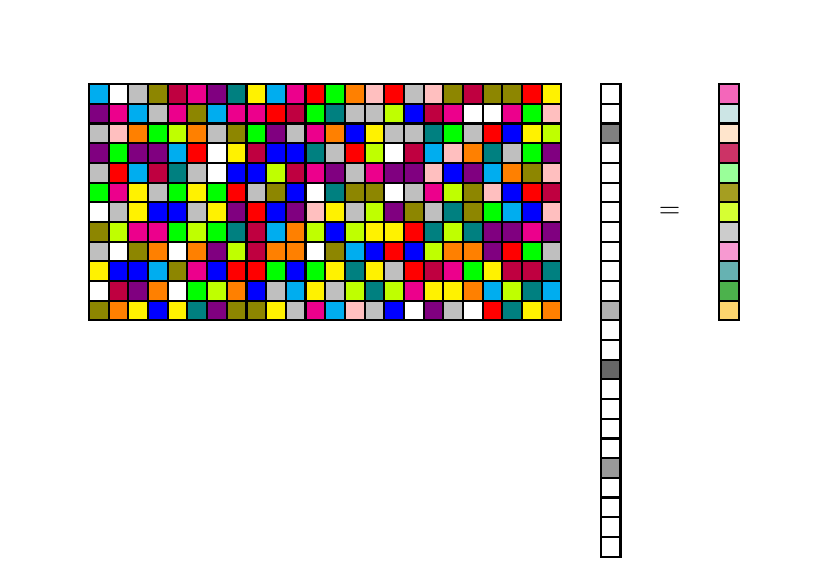
\begin{tikzpicture}
[draw=black, line width=0.75pt,
entry/.style={rectangle, draw, inner sep=0pt, minimum size=2.5mm},
symbol/.style={rectangle, draw, inner sep=0pt, minimum size=2.5mm}]

\node[entry, fill=olive] (x0y0) at (0.0,0.0) {};
\node[entry, fill=white] (x0y1) at (0.0,0.25) {};
\node[entry, fill=yellow] (x0y2) at (0.0,0.5) {};
\node[entry, fill=lightgray] (x0y3) at (0.0,0.75) {};
\node[entry, fill=olive] (x0y4) at (0.0,1.0) {};
\node[entry, fill=white] (x0y5) at (0.0,1.25) {};
\node[entry, fill=green] (x0y6) at (0.0,1.5) {};
\node[entry, fill=lightgray] (x0y7) at (0.0,1.75) {};
\node[entry, fill=violet] (x0y8) at (0.0,2.0) {};
\node[entry, fill=lightgray] (x0y9) at (0.0,2.25) {};
\node[entry, fill=violet] (x0y10) at (0.0,2.5) {};
\node[entry, fill=cyan] (x0y11) at (0.0,2.75) {};

\node[entry, fill=orange] (x1y0) at (0.25,0.0) {};
\node[entry, fill=purple] (x1y1) at (0.25,0.25) {};
\node[entry, fill=blue] (x1y2) at (0.25,0.5) {};
\node[entry, fill=white] (x1y3) at (0.25,0.75) {};
\node[entry, fill=lime] (x1y4) at (0.25,1.0) {};
\node[entry, fill=lightgray] (x1y5) at (0.25,1.25) {};
\node[entry, fill=magenta] (x1y6) at (0.25,1.5) {};
\node[entry, fill=red] (x1y7) at (0.25,1.75) {};
\node[entry, fill=green] (x1y8) at (0.25,2.0) {};
\node[entry, fill=pink] (x1y9) at (0.25,2.25) {};
\node[entry, fill=magenta] (x1y10) at (0.25,2.5) {};
\node[entry, fill=white] (x1y11) at (0.25,2.75) {};

\node[entry, fill=yellow] (x2y0) at (0.5,0.0) {};
\node[entry, fill=violet] (x2y1) at (0.5,0.25) {};
\node[entry, fill=blue] (x2y2) at (0.5,0.5) {};
\node[entry, fill=olive] (x2y3) at (0.5,0.75) {};
\node[entry, fill=magenta] (x2y4) at (0.5,1.0) {};
\node[entry, fill=yellow] (x2y5) at (0.5,1.25) {};
\node[entry, fill=yellow] (x2y6) at (0.5,1.5) {};
\node[entry, fill=cyan] (x2y7) at (0.5,1.75) {};
\node[entry, fill=violet] (x2y8) at (0.5,2.0) {};
\node[entry, fill=orange] (x2y9) at (0.5,2.25) {};
\node[entry, fill=cyan] (x2y10) at (0.5,2.5) {};
\node[entry, fill=lightgray] (x2y11) at (0.5,2.75) {};

\node[entry, fill=blue] (x3y0) at (0.75,0.0) {};
\node[entry, fill=orange] (x3y1) at (0.75,0.25) {};
\node[entry, fill=cyan] (x3y2) at (0.75,0.5) {};
\node[entry, fill=orange] (x3y3) at (0.75,0.75) {};
\node[entry, fill=magenta] (x3y4) at (0.75,1.0) {};
\node[entry, fill=blue] (x3y5) at (0.75,1.25) {};
\node[entry, fill=lightgray] (x3y6) at (0.75,1.5) {};
\node[entry, fill=purple] (x3y7) at (0.75,1.75) {};
\node[entry, fill=violet] (x3y8) at (0.75,2.0) {};
\node[entry, fill=green] (x3y9) at (0.75,2.25) {};
\node[entry, fill=lightgray] (x3y10) at (0.75,2.5) {};
\node[entry, fill=olive] (x3y11) at (0.75,2.75) {};

\node[entry, fill=yellow] (x4y0) at (1.0,0.0) {};
\node[entry, fill=white] (x4y1) at (1.0,0.25) {};
\node[entry, fill=olive] (x4y2) at (1.0,0.5) {};
\node[entry, fill=white] (x4y3) at (1.0,0.75) {};
\node[entry, fill=green] (x4y4) at (1.0,1.0) {};
\node[entry, fill=blue] (x4y5) at (1.0,1.25) {};
\node[entry, fill=green] (x4y6) at (1.0,1.5) {};
\node[entry, fill=teal] (x4y7) at (1.0,1.75) {};
\node[entry, fill=cyan] (x4y8) at (1.0,2.0) {};
\node[entry, fill=lime] (x4y9) at (1.0,2.25) {};
\node[entry, fill=magenta] (x4y10) at (1.0,2.5) {};
\node[entry, fill=purple] (x4y11) at (1.0,2.75) {};

\node[entry, fill=teal] (x5y0) at (1.25,0.0) {};
\node[entry, fill=green] (x5y1) at (1.25,0.25) {};
\node[entry, fill=magenta] (x5y2) at (1.25,0.5) {};
\node[entry, fill=orange] (x5y3) at (1.25,0.75) {};
\node[entry, fill=lime] (x5y4) at (1.25,1.0) {};
\node[entry, fill=lightgray] (x5y5) at (1.25,1.25) {};
\node[entry, fill=yellow] (x5y6) at (1.25,1.5) {};
\node[entry, fill=lightgray] (x5y7) at (1.25,1.75) {};
\node[entry, fill=red] (x5y8) at (1.25,2.0) {};
\node[entry, fill=orange] (x5y9) at (1.25,2.25) {};
\node[entry, fill=olive] (x5y10) at (1.25,2.5) {};
\node[entry, fill=magenta] (x5y11) at (1.25,2.75) {};

\node[entry, fill=violet] (x6y0) at (1.5,0.0) {};
\node[entry, fill=lime] (x6y1) at (1.5,0.25) {};
\node[entry, fill=blue] (x6y2) at (1.5,0.5) {};
\node[entry, fill=violet] (x6y3) at (1.5,0.75) {};
\node[entry, fill=green] (x6y4) at (1.5,1.0) {};
\node[entry, fill=yellow] (x6y5) at (1.5,1.25) {};
\node[entry, fill=green] (x6y6) at (1.5,1.5) {};
\node[entry, fill=white] (x6y7) at (1.5,1.75) {};
\node[entry, fill=white] (x6y8) at (1.5,2.0) {};
\node[entry, fill=lightgray] (x6y9) at (1.5,2.25) {};
\node[entry, fill=cyan] (x6y10) at (1.5,2.5) {};
\node[entry, fill=violet] (x6y11) at (1.5,2.75) {};

\node[entry, fill=olive] (x7y0) at (1.75,0.0) {};
\node[entry, fill=orange] (x7y1) at (1.75,0.25) {};
\node[entry, fill=red] (x7y2) at (1.75,0.5) {};
\node[entry, fill=lime] (x7y3) at (1.75,0.75) {};
\node[entry, fill=teal] (x7y4) at (1.75,1.0) {};
\node[entry, fill=violet] (x7y5) at (1.75,1.25) {};
\node[entry, fill=red] (x7y6) at (1.75,1.5) {};
\node[entry, fill=blue] (x7y7) at (1.75,1.75) {};
\node[entry, fill=yellow] (x7y8) at (1.75,2.0) {};
\node[entry, fill=olive] (x7y9) at (1.75,2.25) {};
\node[entry, fill=magenta] (x7y10) at (1.75,2.5) {};
\node[entry, fill=teal] (x7y11) at (1.75,2.75) {};

\node[entry, fill=olive] (x8y0) at (2.0,0.0) {};
\node[entry, fill=blue] (x8y1) at (2.0,0.25) {};
\node[entry, fill=red] (x8y2) at (2.0,0.5) {};
\node[entry, fill=purple] (x8y3) at (2.0,0.75) {};
\node[entry, fill=purple] (x8y4) at (2.0,1.0) {};
\node[entry, fill=red] (x8y5) at (2.0,1.25) {};
\node[entry, fill=lightgray] (x8y6) at (2.0,1.5) {};
\node[entry, fill=blue] (x8y7) at (2.0,1.75) {};
\node[entry, fill=purple] (x8y8) at (2.0,2.0) {};
\node[entry, fill=green] (x8y9) at (2.0,2.25) {};
\node[entry, fill=magenta] (x8y10) at (2.0,2.5) {};
\node[entry, fill=yellow] (x8y11) at (2.0,2.75) {};

\node[entry, fill=yellow] (x9y0) at (2.25,0.0) {};
\node[entry, fill=lightgray] (x9y1) at (2.25,0.25) {};
\node[entry, fill=green] (x9y2) at (2.25,0.5) {};
\node[entry, fill=orange] (x9y3) at (2.25,0.75) {};
\node[entry, fill=cyan] (x9y4) at (2.25,1.0) {};
\node[entry, fill=blue] (x9y5) at (2.25,1.25) {};
\node[entry, fill=olive] (x9y6) at (2.25,1.5) {};
\node[entry, fill=lime] (x9y7) at (2.25,1.75) {};
\node[entry, fill=blue] (x9y8) at (2.25,2.0) {};
\node[entry, fill=violet] (x9y9) at (2.25,2.25) {};
\node[entry, fill=red] (x9y10) at (2.25,2.5) {};
\node[entry, fill=cyan] (x9y11) at (2.25,2.75) {};

\node[entry, fill=lightgray] (x10y0) at (2.5,0.0) {};
\node[entry, fill=cyan] (x10y1) at (2.5,0.25) {};
\node[entry, fill=blue] (x10y2) at (2.5,0.5) {};
\node[entry, fill=orange] (x10y3) at (2.5,0.75) {};
\node[entry, fill=orange] (x10y4) at (2.5,1.0) {};
\node[entry, fill=violet] (x10y5) at (2.5,1.25) {};
\node[entry, fill=blue] (x10y6) at (2.5,1.5) {};
\node[entry, fill=purple] (x10y7) at (2.5,1.75) {};
\node[entry, fill=blue] (x10y8) at (2.5,2.0) {};
\node[entry, fill=lightgray] (x10y9) at (2.5,2.25) {};
\node[entry, fill=purple] (x10y10) at (2.5,2.5) {};
\node[entry, fill=magenta] (x10y11) at (2.5,2.75) {};

\node[entry, fill=magenta] (x11y0) at (2.75,0.0) {};
\node[entry, fill=yellow] (x11y1) at (2.75,0.25) {};
\node[entry, fill=green] (x11y2) at (2.75,0.5) {};
\node[entry, fill=white] (x11y3) at (2.75,0.75) {};
\node[entry, fill=lime] (x11y4) at (2.75,1.0) {};
\node[entry, fill=pink] (x11y5) at (2.75,1.25) {};
\node[entry, fill=white] (x11y6) at (2.75,1.5) {};
\node[entry, fill=magenta] (x11y7) at (2.75,1.75) {};
\node[entry, fill=teal] (x11y8) at (2.75,2.0) {};
\node[entry, fill=magenta] (x11y9) at (2.75,2.25) {};
\node[entry, fill=green] (x11y10) at (2.75,2.5) {};
\node[entry, fill=red] (x11y11) at (2.75,2.75) {};

\node[entry, fill=cyan] (x12y0) at (3.0,0.0) {};
\node[entry, fill=lightgray] (x12y1) at (3.0,0.25) {};
\node[entry, fill=yellow] (x12y2) at (3.0,0.5) {};
\node[entry, fill=olive] (x12y3) at (3.0,0.75) {};
\node[entry, fill=blue] (x12y4) at (3.0,1.0) {};
\node[entry, fill=yellow] (x12y5) at (3.0,1.25) {};
\node[entry, fill=teal] (x12y6) at (3.0,1.5) {};
\node[entry, fill=violet] (x12y7) at (3.0,1.75) {};
\node[entry, fill=lightgray] (x12y8) at (3.0,2.0) {};
\node[entry, fill=orange] (x12y9) at (3.0,2.25) {};
\node[entry, fill=teal] (x12y10) at (3.0,2.5) {};
\node[entry, fill=green] (x12y11) at (3.0,2.75) {};

\node[entry, fill=pink] (x13y0) at (3.25,0.0) {};
\node[entry, fill=lime] (x13y1) at (3.25,0.25) {};
\node[entry, fill=teal] (x13y2) at (3.25,0.5) {};
\node[entry, fill=cyan] (x13y3) at (3.25,0.75) {};
\node[entry, fill=lime] (x13y4) at (3.25,1.0) {};
\node[entry, fill=lightgray] (x13y5) at (3.25,1.25) {};
\node[entry, fill=olive] (x13y6) at (3.25,1.5) {};
\node[entry, fill=lightgray] (x13y7) at (3.25,1.75) {};
\node[entry, fill=red] (x13y8) at (3.25,2.0) {};
\node[entry, fill=blue] (x13y9) at (3.25,2.25) {};
\node[entry, fill=lightgray] (x13y10) at (3.25,2.5) {};
\node[entry, fill=orange] (x13y11) at (3.25,2.75) {};

\node[entry, fill=lightgray] (x14y0) at (3.5,0.0) {};
\node[entry, fill=teal] (x14y1) at (3.5,0.25) {};
\node[entry, fill=yellow] (x14y2) at (3.5,0.5) {};
\node[entry, fill=blue] (x14y3) at (3.5,0.75) {};
\node[entry, fill=yellow] (x14y4) at (3.5,1.0) {};
\node[entry, fill=lime] (x14y5) at (3.5,1.25) {};
\node[entry, fill=olive] (x14y6) at (3.5,1.5) {};
\node[entry, fill=magenta] (x14y7) at (3.5,1.75) {};
\node[entry, fill=lime] (x14y8) at (3.5,2.0) {};
\node[entry, fill=yellow] (x14y9) at (3.5,2.25) {};
\node[entry, fill=lightgray] (x14y10) at (3.5,2.5) {};
\node[entry, fill=pink] (x14y11) at (3.5,2.75) {};

\node[entry, fill=blue] (x15y0) at (3.75,0.0) {};
\node[entry, fill=lime] (x15y1) at (3.75,0.25) {};
\node[entry, fill=lightgray] (x15y2) at (3.75,0.5) {};
\node[entry, fill=red] (x15y3) at (3.75,0.75) {};
\node[entry, fill=yellow] (x15y4) at (3.75,1.0) {};
\node[entry, fill=violet] (x15y5) at (3.75,1.25) {};
\node[entry, fill=white] (x15y6) at (3.75,1.5) {};
\node[entry, fill=violet] (x15y7) at (3.75,1.75) {};
\node[entry, fill=white] (x15y8) at (3.75,2.0) {};
\node[entry, fill=lightgray] (x15y9) at (3.75,2.25) {};
\node[entry, fill=lime] (x15y10) at (3.75,2.5) {};
\node[entry, fill=red] (x15y11) at (3.75,2.75) {};

\node[entry, fill=white] (x16y0) at (4.0,0.0) {};
\node[entry, fill=magenta] (x16y1) at (4.0,0.25) {};
\node[entry, fill=red] (x16y2) at (4.0,0.5) {};
\node[entry, fill=blue] (x16y3) at (4.0,0.75) {};
\node[entry, fill=red] (x16y4) at (4.0,1.0) {};
\node[entry, fill=olive] (x16y5) at (4.0,1.25) {};
\node[entry, fill=lightgray] (x16y6) at (4.0,1.5) {};
\node[entry, fill=violet] (x16y7) at (4.0,1.75) {};
\node[entry, fill=purple] (x16y8) at (4.0,2.0) {};
\node[entry, fill=lightgray] (x16y9) at (4.0,2.25) {};
\node[entry, fill=blue] (x16y10) at (4.0,2.5) {};
\node[entry, fill=lightgray] (x16y11) at (4.0,2.75) {};

\node[entry, fill=violet] (x17y0) at (4.25,0.0) {};
\node[entry, fill=yellow] (x17y1) at (4.25,0.25) {};
\node[entry, fill=purple] (x17y2) at (4.25,0.5) {};
\node[entry, fill=lime] (x17y3) at (4.25,0.75) {};
\node[entry, fill=teal] (x17y4) at (4.25,1.0) {};
\node[entry, fill=lightgray] (x17y5) at (4.25,1.25) {};
\node[entry, fill=magenta] (x17y6) at (4.25,1.5) {};
\node[entry, fill=pink] (x17y7) at (4.25,1.75) {};
\node[entry, fill=cyan] (x17y8) at (4.25,2.0) {};
\node[entry, fill=teal] (x17y9) at (4.25,2.25) {};
\node[entry, fill=purple] (x17y10) at (4.25,2.5) {};
\node[entry, fill=pink] (x17y11) at (4.25,2.75) {};

\node[entry, fill=lightgray] (x18y0) at (4.5,0.0) {};
\node[entry, fill=yellow] (x18y1) at (4.5,0.25) {};
\node[entry, fill=magenta] (x18y2) at (4.5,0.5) {};
\node[entry, fill=orange] (x18y3) at (4.5,0.75) {};
\node[entry, fill=lime] (x18y4) at (4.5,1.0) {};
\node[entry, fill=teal] (x18y5) at (4.5,1.25) {};
\node[entry, fill=lime] (x18y6) at (4.5,1.5) {};
\node[entry, fill=blue] (x18y7) at (4.5,1.75) {};
\node[entry, fill=pink] (x18y8) at (4.5,2.0) {};
\node[entry, fill=green] (x18y9) at (4.5,2.25) {};
\node[entry, fill=magenta] (x18y10) at (4.5,2.5) {};
\node[entry, fill=olive] (x18y11) at (4.5,2.75) {};

\node[entry, fill=white] (x19y0) at (4.75,0.0) {};
\node[entry, fill=orange] (x19y1) at (4.75,0.25) {};
\node[entry, fill=green] (x19y2) at (4.75,0.5) {};
\node[entry, fill=orange] (x19y3) at (4.75,0.75) {};
\node[entry, fill=teal] (x19y4) at (4.75,1.0) {};
\node[entry, fill=olive] (x19y5) at (4.75,1.25) {};
\node[entry, fill=olive] (x19y6) at (4.75,1.5) {};
\node[entry, fill=violet] (x19y7) at (4.75,1.75) {};
\node[entry, fill=orange] (x19y8) at (4.75,2.0) {};
\node[entry, fill=lightgray] (x19y9) at (4.75,2.25) {};
\node[entry, fill=white] (x19y10) at (4.75,2.5) {};
\node[entry, fill=purple] (x19y11) at (4.75,2.75) {};

\node[entry, fill=red] (x20y0) at (5.0,0.0) {};
\node[entry, fill=cyan] (x20y1) at (5.0,0.25) {};
\node[entry, fill=yellow] (x20y2) at (5.0,0.5) {};
\node[entry, fill=violet] (x20y3) at (5.0,0.75) {};
\node[entry, fill=violet] (x20y4) at (5.0,1.0) {};
\node[entry, fill=green] (x20y5) at (5.0,1.25) {};
\node[entry, fill=pink] (x20y6) at (5.0,1.5) {};
\node[entry, fill=cyan] (x20y7) at (5.0,1.75) {};
\node[entry, fill=teal] (x20y8) at (5.0,2.0) {};
\node[entry, fill=red] (x20y9) at (5.0,2.25) {};
\node[entry, fill=white] (x20y10) at (5.0,2.5) {};
\node[entry, fill=olive] (x20y11) at (5.0,2.75) {};

\node[entry, fill=teal] (x21y0) at (5.25,0.0) {};
\node[entry, fill=lime] (x21y1) at (5.25,0.25) {};
\node[entry, fill=purple] (x21y2) at (5.25,0.5) {};
\node[entry, fill=red] (x21y3) at (5.25,0.75) {};
\node[entry, fill=violet] (x21y4) at (5.25,1.0) {};
\node[entry, fill=cyan] (x21y5) at (5.25,1.25) {};
\node[entry, fill=blue] (x21y6) at (5.25,1.5) {};
\node[entry, fill=orange] (x21y7) at (5.25,1.75) {};
\node[entry, fill=lightgray] (x21y8) at (5.25,2.0) {};
\node[entry, fill=blue] (x21y9) at (5.25,2.25) {};
\node[entry, fill=magenta] (x21y10) at (5.25,2.5) {};
\node[entry, fill=olive] (x21y11) at (5.25,2.75) {};

\node[entry, fill=yellow] (x22y0) at (5.5,0.0) {};
\node[entry, fill=teal] (x22y1) at (5.5,0.25) {};
\node[entry, fill=purple] (x22y2) at (5.5,0.5) {};
\node[entry, fill=green] (x22y3) at (5.5,0.75) {};
\node[entry, fill=magenta] (x22y4) at (5.5,1.0) {};
\node[entry, fill=blue] (x22y5) at (5.5,1.25) {};
\node[entry, fill=red] (x22y6) at (5.5,1.5) {};
\node[entry, fill=olive] (x22y7) at (5.5,1.75) {};
\node[entry, fill=green] (x22y8) at (5.5,2.0) {};
\node[entry, fill=yellow] (x22y9) at (5.5,2.25) {};
\node[entry, fill=green] (x22y10) at (5.5,2.5) {};
\node[entry, fill=red] (x22y11) at (5.5,2.75) {};

\node[entry, fill=orange] (x23y0) at (5.75,0.0) {};
\node[entry, fill=cyan] (x23y1) at (5.75,0.25) {};
\node[entry, fill=teal] (x23y2) at (5.75,0.5) {};
\node[entry, fill=lightgray] (x23y3) at (5.75,0.75) {};
\node[entry, fill=violet] (x23y4) at (5.75,1.0) {};
\node[entry, fill=pink] (x23y5) at (5.75,1.25) {};
\node[entry, fill=purple] (x23y6) at (5.75,1.5) {};
\node[entry, fill=pink] (x23y7) at (5.75,1.75) {};
\node[entry, fill=violet] (x23y8) at (5.75,2.0) {};
\node[entry, fill=lime] (x23y9) at (5.75,2.25) {};
\node[entry, fill=pink] (x23y10) at (5.75,2.5) {};
\node[entry, fill=yellow] (x23y11) at (5.75,2.75) {};

\node[symbol] (s01) at (6.5,-3.00) {};
\node[symbol] (s02) at (6.5,-2.75) {};
\node[symbol] (s03) at (6.5,-2.50) {};
\node[symbol] (s04) at (6.5,-2.25) {};
\node[symbol,fill=black!40] (s05) at (6.5,-2.00) {};
\node[symbol] (s06) at (6.5,-1.75) {};
\node[symbol] (s07) at (6.5,-1.50) {};
\node[symbol] (s08) at (6.5,-1.25) {};
\node[symbol] (s09) at (6.5,-1.00) {};
\node[symbol,fill=black!60] (s10) at (6.5,-0.75) {};
\node[symbol] (s11) at (6.5,-0.50) {};
\node[symbol] (s12) at (6.5,-0.25) {};
\node[symbol,fill=black!30] (s13) at (6.5,0) {};
\node[symbol] (s14) at (6.5,0.25) {};
\node[symbol] (s15) at (6.5,0.50) {};
\node[symbol] (s16) at (6.5,0.75) {};
\node[symbol] (s17) at (6.5,1.00) {};
\node[symbol] (s18) at (6.5,1.25) {};
\node[symbol] (s19) at (6.5,1.50) {};
\node[symbol] (s20) at (6.5,1.75) {};
\node[symbol] (s21) at (6.5,2.00) {};
\node[symbol,fill=black!50] (s22) at (6.5,2.25) {};
\node[symbol] (s23) at (6.5,2.50) {};
\node[symbol] (s24) at (6.5,2.75) {};

\node (equal) at (7.25,1.25) {$=$};

\node[entry, fill=yellow!40!pink] (o0) at (8,0.0) {};
\node[entry, fill=gray!60!green] (o1) at (8,0.25) {};
\node[entry, fill=teal!60] (o2) at (8,0.5) {};
\node[entry, fill=magenta!40] (o3) at (8,0.75) {};
\node[entry, fill=gray!40] (o4) at (8,1.0) {};
\node[entry, fill=green!20!yellow!80] (o5) at (8,1.25) {};
\node[entry, fill=olive!80] (o6) at (8,1.5) {};
\node[entry, fill=green!40] (o7) at (8,1.75) {};
\node[entry, fill=purple!80] (o8) at (8,2.0) {};
\node[entry, fill=orange!20] (o9) at (8,2.25) {};
\node[entry, fill=teal!20] (o10) at (8,2.5) {};
\node[entry, fill=magenta!60] (o11) at (8,2.75) {};

\draw[|-|,opacity=0] (-0.125, 3.125) to node[above] {\small Number of columns} (5.875, 3.125);
\draw[|-|,opacity=0] (-0.375, -0.125) to node[above,rotate=90] {\small Number of samples} (-0.375, 2.875);
\draw[|-|,opacity=0] (6.875, -3.125) to node[above,rotate=-90] {\small Number of non-zero entries} (6.875, 2.875);
\node[opacity=0] (framework) at (2.875,-0.5) {Sensing matrix $\boldsymbol{\Phi}$};
\node[rotate=-90,opacity=0] (vector) at (7,-0.75) {Sparse vector $\mathbf{s}$};
\node[rotate=-90,opacity=0] (observation) at (8.5,1.5) {Observation $\mathbf{y}$};
\end{tikzpicture}
}
\vspace{-1cm}

\begin{columns}
\column{.80\textwidth}
\begin{block}{Approximate message passing (AMP)}
\blockmathspace
\begin{align*}
\zv^{(t)} &= \yv - \boldsymbol{\Phi} \sv^{(t)} + \textcolor{lightgray}{\overbrace{\frac{\zv^{(t-1)}}{n} \| \sv^{(t)} \|_0}^{\text{Onsager}}} \\
\sv^{(t+1)} &= \etav \big( \boldsymbol{\Phi}^{\transpose} \zv^{(t)} + \sv^{(t)} \big)
\end{align*}
where $\etav (\sv)_k = (|\sv_k| - \alpha \lambda)_+ \operatorname{sgn}(\sv_k)$, \textcolor{lightgray}{$\sv^{(0)} = \zerov$, $\zv^{(0)} = \yv$}
\end{block}
\column{.15\textwidth}
\end{columns}
% % % % %
\vfill
% % % % %
\begin{itemize}
\item Application to high-dimensional spaces
\item Low complexity, scalable framework
\end{itemize}
% % % % %
\end{frame}

% % % % % % % % % % % % % % % % % % % %


\begin{frame}
\frametitle{Compressed Sensing -- AMP}
% % % % %
\hfill
\scalebox{0.5}{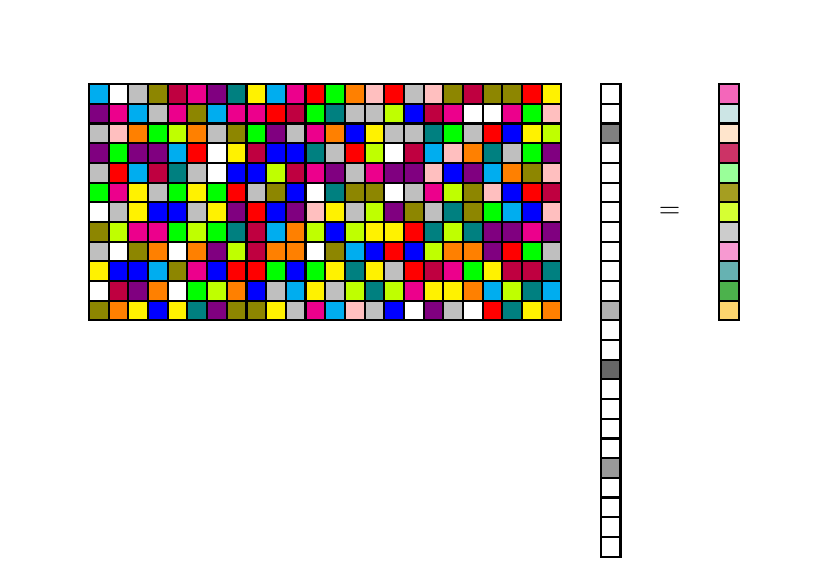
\begin{tikzpicture}
[draw=black, line width=0.75pt,
entry/.style={rectangle, draw, inner sep=0pt, minimum size=2.5mm},
symbol/.style={rectangle, draw, inner sep=0pt, minimum size=2.5mm}]

\node[entry, fill=olive] (x0y0) at (0.0,0.0) {};
\node[entry, fill=white] (x0y1) at (0.0,0.25) {};
\node[entry, fill=yellow] (x0y2) at (0.0,0.5) {};
\node[entry, fill=lightgray] (x0y3) at (0.0,0.75) {};
\node[entry, fill=olive] (x0y4) at (0.0,1.0) {};
\node[entry, fill=white] (x0y5) at (0.0,1.25) {};
\node[entry, fill=green] (x0y6) at (0.0,1.5) {};
\node[entry, fill=lightgray] (x0y7) at (0.0,1.75) {};
\node[entry, fill=violet] (x0y8) at (0.0,2.0) {};
\node[entry, fill=lightgray] (x0y9) at (0.0,2.25) {};
\node[entry, fill=violet] (x0y10) at (0.0,2.5) {};
\node[entry, fill=cyan] (x0y11) at (0.0,2.75) {};

\node[entry, fill=orange] (x1y0) at (0.25,0.0) {};
\node[entry, fill=purple] (x1y1) at (0.25,0.25) {};
\node[entry, fill=blue] (x1y2) at (0.25,0.5) {};
\node[entry, fill=white] (x1y3) at (0.25,0.75) {};
\node[entry, fill=lime] (x1y4) at (0.25,1.0) {};
\node[entry, fill=lightgray] (x1y5) at (0.25,1.25) {};
\node[entry, fill=magenta] (x1y6) at (0.25,1.5) {};
\node[entry, fill=red] (x1y7) at (0.25,1.75) {};
\node[entry, fill=green] (x1y8) at (0.25,2.0) {};
\node[entry, fill=pink] (x1y9) at (0.25,2.25) {};
\node[entry, fill=magenta] (x1y10) at (0.25,2.5) {};
\node[entry, fill=white] (x1y11) at (0.25,2.75) {};

\node[entry, fill=yellow] (x2y0) at (0.5,0.0) {};
\node[entry, fill=violet] (x2y1) at (0.5,0.25) {};
\node[entry, fill=blue] (x2y2) at (0.5,0.5) {};
\node[entry, fill=olive] (x2y3) at (0.5,0.75) {};
\node[entry, fill=magenta] (x2y4) at (0.5,1.0) {};
\node[entry, fill=yellow] (x2y5) at (0.5,1.25) {};
\node[entry, fill=yellow] (x2y6) at (0.5,1.5) {};
\node[entry, fill=cyan] (x2y7) at (0.5,1.75) {};
\node[entry, fill=violet] (x2y8) at (0.5,2.0) {};
\node[entry, fill=orange] (x2y9) at (0.5,2.25) {};
\node[entry, fill=cyan] (x2y10) at (0.5,2.5) {};
\node[entry, fill=lightgray] (x2y11) at (0.5,2.75) {};

\node[entry, fill=blue] (x3y0) at (0.75,0.0) {};
\node[entry, fill=orange] (x3y1) at (0.75,0.25) {};
\node[entry, fill=cyan] (x3y2) at (0.75,0.5) {};
\node[entry, fill=orange] (x3y3) at (0.75,0.75) {};
\node[entry, fill=magenta] (x3y4) at (0.75,1.0) {};
\node[entry, fill=blue] (x3y5) at (0.75,1.25) {};
\node[entry, fill=lightgray] (x3y6) at (0.75,1.5) {};
\node[entry, fill=purple] (x3y7) at (0.75,1.75) {};
\node[entry, fill=violet] (x3y8) at (0.75,2.0) {};
\node[entry, fill=green] (x3y9) at (0.75,2.25) {};
\node[entry, fill=lightgray] (x3y10) at (0.75,2.5) {};
\node[entry, fill=olive] (x3y11) at (0.75,2.75) {};

\node[entry, fill=yellow] (x4y0) at (1.0,0.0) {};
\node[entry, fill=white] (x4y1) at (1.0,0.25) {};
\node[entry, fill=olive] (x4y2) at (1.0,0.5) {};
\node[entry, fill=white] (x4y3) at (1.0,0.75) {};
\node[entry, fill=green] (x4y4) at (1.0,1.0) {};
\node[entry, fill=blue] (x4y5) at (1.0,1.25) {};
\node[entry, fill=green] (x4y6) at (1.0,1.5) {};
\node[entry, fill=teal] (x4y7) at (1.0,1.75) {};
\node[entry, fill=cyan] (x4y8) at (1.0,2.0) {};
\node[entry, fill=lime] (x4y9) at (1.0,2.25) {};
\node[entry, fill=magenta] (x4y10) at (1.0,2.5) {};
\node[entry, fill=purple] (x4y11) at (1.0,2.75) {};

\node[entry, fill=teal] (x5y0) at (1.25,0.0) {};
\node[entry, fill=green] (x5y1) at (1.25,0.25) {};
\node[entry, fill=magenta] (x5y2) at (1.25,0.5) {};
\node[entry, fill=orange] (x5y3) at (1.25,0.75) {};
\node[entry, fill=lime] (x5y4) at (1.25,1.0) {};
\node[entry, fill=lightgray] (x5y5) at (1.25,1.25) {};
\node[entry, fill=yellow] (x5y6) at (1.25,1.5) {};
\node[entry, fill=lightgray] (x5y7) at (1.25,1.75) {};
\node[entry, fill=red] (x5y8) at (1.25,2.0) {};
\node[entry, fill=orange] (x5y9) at (1.25,2.25) {};
\node[entry, fill=olive] (x5y10) at (1.25,2.5) {};
\node[entry, fill=magenta] (x5y11) at (1.25,2.75) {};

\node[entry, fill=violet] (x6y0) at (1.5,0.0) {};
\node[entry, fill=lime] (x6y1) at (1.5,0.25) {};
\node[entry, fill=blue] (x6y2) at (1.5,0.5) {};
\node[entry, fill=violet] (x6y3) at (1.5,0.75) {};
\node[entry, fill=green] (x6y4) at (1.5,1.0) {};
\node[entry, fill=yellow] (x6y5) at (1.5,1.25) {};
\node[entry, fill=green] (x6y6) at (1.5,1.5) {};
\node[entry, fill=white] (x6y7) at (1.5,1.75) {};
\node[entry, fill=white] (x6y8) at (1.5,2.0) {};
\node[entry, fill=lightgray] (x6y9) at (1.5,2.25) {};
\node[entry, fill=cyan] (x6y10) at (1.5,2.5) {};
\node[entry, fill=violet] (x6y11) at (1.5,2.75) {};

\node[entry, fill=olive] (x7y0) at (1.75,0.0) {};
\node[entry, fill=orange] (x7y1) at (1.75,0.25) {};
\node[entry, fill=red] (x7y2) at (1.75,0.5) {};
\node[entry, fill=lime] (x7y3) at (1.75,0.75) {};
\node[entry, fill=teal] (x7y4) at (1.75,1.0) {};
\node[entry, fill=violet] (x7y5) at (1.75,1.25) {};
\node[entry, fill=red] (x7y6) at (1.75,1.5) {};
\node[entry, fill=blue] (x7y7) at (1.75,1.75) {};
\node[entry, fill=yellow] (x7y8) at (1.75,2.0) {};
\node[entry, fill=olive] (x7y9) at (1.75,2.25) {};
\node[entry, fill=magenta] (x7y10) at (1.75,2.5) {};
\node[entry, fill=teal] (x7y11) at (1.75,2.75) {};

\node[entry, fill=olive] (x8y0) at (2.0,0.0) {};
\node[entry, fill=blue] (x8y1) at (2.0,0.25) {};
\node[entry, fill=red] (x8y2) at (2.0,0.5) {};
\node[entry, fill=purple] (x8y3) at (2.0,0.75) {};
\node[entry, fill=purple] (x8y4) at (2.0,1.0) {};
\node[entry, fill=red] (x8y5) at (2.0,1.25) {};
\node[entry, fill=lightgray] (x8y6) at (2.0,1.5) {};
\node[entry, fill=blue] (x8y7) at (2.0,1.75) {};
\node[entry, fill=purple] (x8y8) at (2.0,2.0) {};
\node[entry, fill=green] (x8y9) at (2.0,2.25) {};
\node[entry, fill=magenta] (x8y10) at (2.0,2.5) {};
\node[entry, fill=yellow] (x8y11) at (2.0,2.75) {};

\node[entry, fill=yellow] (x9y0) at (2.25,0.0) {};
\node[entry, fill=lightgray] (x9y1) at (2.25,0.25) {};
\node[entry, fill=green] (x9y2) at (2.25,0.5) {};
\node[entry, fill=orange] (x9y3) at (2.25,0.75) {};
\node[entry, fill=cyan] (x9y4) at (2.25,1.0) {};
\node[entry, fill=blue] (x9y5) at (2.25,1.25) {};
\node[entry, fill=olive] (x9y6) at (2.25,1.5) {};
\node[entry, fill=lime] (x9y7) at (2.25,1.75) {};
\node[entry, fill=blue] (x9y8) at (2.25,2.0) {};
\node[entry, fill=violet] (x9y9) at (2.25,2.25) {};
\node[entry, fill=red] (x9y10) at (2.25,2.5) {};
\node[entry, fill=cyan] (x9y11) at (2.25,2.75) {};

\node[entry, fill=lightgray] (x10y0) at (2.5,0.0) {};
\node[entry, fill=cyan] (x10y1) at (2.5,0.25) {};
\node[entry, fill=blue] (x10y2) at (2.5,0.5) {};
\node[entry, fill=orange] (x10y3) at (2.5,0.75) {};
\node[entry, fill=orange] (x10y4) at (2.5,1.0) {};
\node[entry, fill=violet] (x10y5) at (2.5,1.25) {};
\node[entry, fill=blue] (x10y6) at (2.5,1.5) {};
\node[entry, fill=purple] (x10y7) at (2.5,1.75) {};
\node[entry, fill=blue] (x10y8) at (2.5,2.0) {};
\node[entry, fill=lightgray] (x10y9) at (2.5,2.25) {};
\node[entry, fill=purple] (x10y10) at (2.5,2.5) {};
\node[entry, fill=magenta] (x10y11) at (2.5,2.75) {};

\node[entry, fill=magenta] (x11y0) at (2.75,0.0) {};
\node[entry, fill=yellow] (x11y1) at (2.75,0.25) {};
\node[entry, fill=green] (x11y2) at (2.75,0.5) {};
\node[entry, fill=white] (x11y3) at (2.75,0.75) {};
\node[entry, fill=lime] (x11y4) at (2.75,1.0) {};
\node[entry, fill=pink] (x11y5) at (2.75,1.25) {};
\node[entry, fill=white] (x11y6) at (2.75,1.5) {};
\node[entry, fill=magenta] (x11y7) at (2.75,1.75) {};
\node[entry, fill=teal] (x11y8) at (2.75,2.0) {};
\node[entry, fill=magenta] (x11y9) at (2.75,2.25) {};
\node[entry, fill=green] (x11y10) at (2.75,2.5) {};
\node[entry, fill=red] (x11y11) at (2.75,2.75) {};

\node[entry, fill=cyan] (x12y0) at (3.0,0.0) {};
\node[entry, fill=lightgray] (x12y1) at (3.0,0.25) {};
\node[entry, fill=yellow] (x12y2) at (3.0,0.5) {};
\node[entry, fill=olive] (x12y3) at (3.0,0.75) {};
\node[entry, fill=blue] (x12y4) at (3.0,1.0) {};
\node[entry, fill=yellow] (x12y5) at (3.0,1.25) {};
\node[entry, fill=teal] (x12y6) at (3.0,1.5) {};
\node[entry, fill=violet] (x12y7) at (3.0,1.75) {};
\node[entry, fill=lightgray] (x12y8) at (3.0,2.0) {};
\node[entry, fill=orange] (x12y9) at (3.0,2.25) {};
\node[entry, fill=teal] (x12y10) at (3.0,2.5) {};
\node[entry, fill=green] (x12y11) at (3.0,2.75) {};

\node[entry, fill=pink] (x13y0) at (3.25,0.0) {};
\node[entry, fill=lime] (x13y1) at (3.25,0.25) {};
\node[entry, fill=teal] (x13y2) at (3.25,0.5) {};
\node[entry, fill=cyan] (x13y3) at (3.25,0.75) {};
\node[entry, fill=lime] (x13y4) at (3.25,1.0) {};
\node[entry, fill=lightgray] (x13y5) at (3.25,1.25) {};
\node[entry, fill=olive] (x13y6) at (3.25,1.5) {};
\node[entry, fill=lightgray] (x13y7) at (3.25,1.75) {};
\node[entry, fill=red] (x13y8) at (3.25,2.0) {};
\node[entry, fill=blue] (x13y9) at (3.25,2.25) {};
\node[entry, fill=lightgray] (x13y10) at (3.25,2.5) {};
\node[entry, fill=orange] (x13y11) at (3.25,2.75) {};

\node[entry, fill=lightgray] (x14y0) at (3.5,0.0) {};
\node[entry, fill=teal] (x14y1) at (3.5,0.25) {};
\node[entry, fill=yellow] (x14y2) at (3.5,0.5) {};
\node[entry, fill=blue] (x14y3) at (3.5,0.75) {};
\node[entry, fill=yellow] (x14y4) at (3.5,1.0) {};
\node[entry, fill=lime] (x14y5) at (3.5,1.25) {};
\node[entry, fill=olive] (x14y6) at (3.5,1.5) {};
\node[entry, fill=magenta] (x14y7) at (3.5,1.75) {};
\node[entry, fill=lime] (x14y8) at (3.5,2.0) {};
\node[entry, fill=yellow] (x14y9) at (3.5,2.25) {};
\node[entry, fill=lightgray] (x14y10) at (3.5,2.5) {};
\node[entry, fill=pink] (x14y11) at (3.5,2.75) {};

\node[entry, fill=blue] (x15y0) at (3.75,0.0) {};
\node[entry, fill=lime] (x15y1) at (3.75,0.25) {};
\node[entry, fill=lightgray] (x15y2) at (3.75,0.5) {};
\node[entry, fill=red] (x15y3) at (3.75,0.75) {};
\node[entry, fill=yellow] (x15y4) at (3.75,1.0) {};
\node[entry, fill=violet] (x15y5) at (3.75,1.25) {};
\node[entry, fill=white] (x15y6) at (3.75,1.5) {};
\node[entry, fill=violet] (x15y7) at (3.75,1.75) {};
\node[entry, fill=white] (x15y8) at (3.75,2.0) {};
\node[entry, fill=lightgray] (x15y9) at (3.75,2.25) {};
\node[entry, fill=lime] (x15y10) at (3.75,2.5) {};
\node[entry, fill=red] (x15y11) at (3.75,2.75) {};

\node[entry, fill=white] (x16y0) at (4.0,0.0) {};
\node[entry, fill=magenta] (x16y1) at (4.0,0.25) {};
\node[entry, fill=red] (x16y2) at (4.0,0.5) {};
\node[entry, fill=blue] (x16y3) at (4.0,0.75) {};
\node[entry, fill=red] (x16y4) at (4.0,1.0) {};
\node[entry, fill=olive] (x16y5) at (4.0,1.25) {};
\node[entry, fill=lightgray] (x16y6) at (4.0,1.5) {};
\node[entry, fill=violet] (x16y7) at (4.0,1.75) {};
\node[entry, fill=purple] (x16y8) at (4.0,2.0) {};
\node[entry, fill=lightgray] (x16y9) at (4.0,2.25) {};
\node[entry, fill=blue] (x16y10) at (4.0,2.5) {};
\node[entry, fill=lightgray] (x16y11) at (4.0,2.75) {};

\node[entry, fill=violet] (x17y0) at (4.25,0.0) {};
\node[entry, fill=yellow] (x17y1) at (4.25,0.25) {};
\node[entry, fill=purple] (x17y2) at (4.25,0.5) {};
\node[entry, fill=lime] (x17y3) at (4.25,0.75) {};
\node[entry, fill=teal] (x17y4) at (4.25,1.0) {};
\node[entry, fill=lightgray] (x17y5) at (4.25,1.25) {};
\node[entry, fill=magenta] (x17y6) at (4.25,1.5) {};
\node[entry, fill=pink] (x17y7) at (4.25,1.75) {};
\node[entry, fill=cyan] (x17y8) at (4.25,2.0) {};
\node[entry, fill=teal] (x17y9) at (4.25,2.25) {};
\node[entry, fill=purple] (x17y10) at (4.25,2.5) {};
\node[entry, fill=pink] (x17y11) at (4.25,2.75) {};

\node[entry, fill=lightgray] (x18y0) at (4.5,0.0) {};
\node[entry, fill=yellow] (x18y1) at (4.5,0.25) {};
\node[entry, fill=magenta] (x18y2) at (4.5,0.5) {};
\node[entry, fill=orange] (x18y3) at (4.5,0.75) {};
\node[entry, fill=lime] (x18y4) at (4.5,1.0) {};
\node[entry, fill=teal] (x18y5) at (4.5,1.25) {};
\node[entry, fill=lime] (x18y6) at (4.5,1.5) {};
\node[entry, fill=blue] (x18y7) at (4.5,1.75) {};
\node[entry, fill=pink] (x18y8) at (4.5,2.0) {};
\node[entry, fill=green] (x18y9) at (4.5,2.25) {};
\node[entry, fill=magenta] (x18y10) at (4.5,2.5) {};
\node[entry, fill=olive] (x18y11) at (4.5,2.75) {};

\node[entry, fill=white] (x19y0) at (4.75,0.0) {};
\node[entry, fill=orange] (x19y1) at (4.75,0.25) {};
\node[entry, fill=green] (x19y2) at (4.75,0.5) {};
\node[entry, fill=orange] (x19y3) at (4.75,0.75) {};
\node[entry, fill=teal] (x19y4) at (4.75,1.0) {};
\node[entry, fill=olive] (x19y5) at (4.75,1.25) {};
\node[entry, fill=olive] (x19y6) at (4.75,1.5) {};
\node[entry, fill=violet] (x19y7) at (4.75,1.75) {};
\node[entry, fill=orange] (x19y8) at (4.75,2.0) {};
\node[entry, fill=lightgray] (x19y9) at (4.75,2.25) {};
\node[entry, fill=white] (x19y10) at (4.75,2.5) {};
\node[entry, fill=purple] (x19y11) at (4.75,2.75) {};

\node[entry, fill=red] (x20y0) at (5.0,0.0) {};
\node[entry, fill=cyan] (x20y1) at (5.0,0.25) {};
\node[entry, fill=yellow] (x20y2) at (5.0,0.5) {};
\node[entry, fill=violet] (x20y3) at (5.0,0.75) {};
\node[entry, fill=violet] (x20y4) at (5.0,1.0) {};
\node[entry, fill=green] (x20y5) at (5.0,1.25) {};
\node[entry, fill=pink] (x20y6) at (5.0,1.5) {};
\node[entry, fill=cyan] (x20y7) at (5.0,1.75) {};
\node[entry, fill=teal] (x20y8) at (5.0,2.0) {};
\node[entry, fill=red] (x20y9) at (5.0,2.25) {};
\node[entry, fill=white] (x20y10) at (5.0,2.5) {};
\node[entry, fill=olive] (x20y11) at (5.0,2.75) {};

\node[entry, fill=teal] (x21y0) at (5.25,0.0) {};
\node[entry, fill=lime] (x21y1) at (5.25,0.25) {};
\node[entry, fill=purple] (x21y2) at (5.25,0.5) {};
\node[entry, fill=red] (x21y3) at (5.25,0.75) {};
\node[entry, fill=violet] (x21y4) at (5.25,1.0) {};
\node[entry, fill=cyan] (x21y5) at (5.25,1.25) {};
\node[entry, fill=blue] (x21y6) at (5.25,1.5) {};
\node[entry, fill=orange] (x21y7) at (5.25,1.75) {};
\node[entry, fill=lightgray] (x21y8) at (5.25,2.0) {};
\node[entry, fill=blue] (x21y9) at (5.25,2.25) {};
\node[entry, fill=magenta] (x21y10) at (5.25,2.5) {};
\node[entry, fill=olive] (x21y11) at (5.25,2.75) {};

\node[entry, fill=yellow] (x22y0) at (5.5,0.0) {};
\node[entry, fill=teal] (x22y1) at (5.5,0.25) {};
\node[entry, fill=purple] (x22y2) at (5.5,0.5) {};
\node[entry, fill=green] (x22y3) at (5.5,0.75) {};
\node[entry, fill=magenta] (x22y4) at (5.5,1.0) {};
\node[entry, fill=blue] (x22y5) at (5.5,1.25) {};
\node[entry, fill=red] (x22y6) at (5.5,1.5) {};
\node[entry, fill=olive] (x22y7) at (5.5,1.75) {};
\node[entry, fill=green] (x22y8) at (5.5,2.0) {};
\node[entry, fill=yellow] (x22y9) at (5.5,2.25) {};
\node[entry, fill=green] (x22y10) at (5.5,2.5) {};
\node[entry, fill=red] (x22y11) at (5.5,2.75) {};

\node[entry, fill=orange] (x23y0) at (5.75,0.0) {};
\node[entry, fill=cyan] (x23y1) at (5.75,0.25) {};
\node[entry, fill=teal] (x23y2) at (5.75,0.5) {};
\node[entry, fill=lightgray] (x23y3) at (5.75,0.75) {};
\node[entry, fill=violet] (x23y4) at (5.75,1.0) {};
\node[entry, fill=pink] (x23y5) at (5.75,1.25) {};
\node[entry, fill=purple] (x23y6) at (5.75,1.5) {};
\node[entry, fill=pink] (x23y7) at (5.75,1.75) {};
\node[entry, fill=violet] (x23y8) at (5.75,2.0) {};
\node[entry, fill=lime] (x23y9) at (5.75,2.25) {};
\node[entry, fill=pink] (x23y10) at (5.75,2.5) {};
\node[entry, fill=yellow] (x23y11) at (5.75,2.75) {};

\node[symbol] (s01) at (6.5,-3.00) {};
\node[symbol] (s02) at (6.5,-2.75) {};
\node[symbol] (s03) at (6.5,-2.50) {};
\node[symbol] (s04) at (6.5,-2.25) {};
\node[symbol,fill=black!40] (s05) at (6.5,-2.00) {};
\node[symbol] (s06) at (6.5,-1.75) {};
\node[symbol] (s07) at (6.5,-1.50) {};
\node[symbol] (s08) at (6.5,-1.25) {};
\node[symbol] (s09) at (6.5,-1.00) {};
\node[symbol,fill=black!60] (s10) at (6.5,-0.75) {};
\node[symbol] (s11) at (6.5,-0.50) {};
\node[symbol] (s12) at (6.5,-0.25) {};
\node[symbol,fill=black!30] (s13) at (6.5,0) {};
\node[symbol] (s14) at (6.5,0.25) {};
\node[symbol] (s15) at (6.5,0.50) {};
\node[symbol] (s16) at (6.5,0.75) {};
\node[symbol] (s17) at (6.5,1.00) {};
\node[symbol] (s18) at (6.5,1.25) {};
\node[symbol] (s19) at (6.5,1.50) {};
\node[symbol] (s20) at (6.5,1.75) {};
\node[symbol] (s21) at (6.5,2.00) {};
\node[symbol,fill=black!50] (s22) at (6.5,2.25) {};
\node[symbol] (s23) at (6.5,2.50) {};
\node[symbol] (s24) at (6.5,2.75) {};

\node (equal) at (7.25,1.25) {$=$};

\node[entry, fill=yellow!40!pink] (o0) at (8,0.0) {};
\node[entry, fill=gray!60!green] (o1) at (8,0.25) {};
\node[entry, fill=teal!60] (o2) at (8,0.5) {};
\node[entry, fill=magenta!40] (o3) at (8,0.75) {};
\node[entry, fill=gray!40] (o4) at (8,1.0) {};
\node[entry, fill=green!20!yellow!80] (o5) at (8,1.25) {};
\node[entry, fill=olive!80] (o6) at (8,1.5) {};
\node[entry, fill=green!40] (o7) at (8,1.75) {};
\node[entry, fill=purple!80] (o8) at (8,2.0) {};
\node[entry, fill=orange!20] (o9) at (8,2.25) {};
\node[entry, fill=teal!20] (o10) at (8,2.5) {};
\node[entry, fill=magenta!60] (o11) at (8,2.75) {};

\draw[|-|,opacity=0] (-0.125, 3.125) to node[above] {\small Number of columns} (5.875, 3.125);
\draw[|-|,opacity=0] (-0.375, -0.125) to node[above,rotate=90] {\small Number of samples} (-0.375, 2.875);
\draw[|-|,opacity=0] (6.875, -3.125) to node[above,rotate=-90] {\small Number of non-zero entries} (6.875, 2.875);
\node[opacity=0] (framework) at (2.875,-0.5) {Sensing matrix $\boldsymbol{\Phi}$};
\node[rotate=-90,opacity=0] (vector) at (7,-0.75) {Sparse vector $\mathbf{s}$};
\node[rotate=-90,opacity=0] (observation) at (8.5,1.5) {Observation $\mathbf{y}$};
\end{tikzpicture}
}
\vspace{-1cm}

\begin{columns}
\column{.80\textwidth}
\begin{block}{Approximate message passing (AMP)}
\blockmathspace
\begin{align*}
\zv^{(t)} &= \yv - \boldsymbol{\Phi} \sv^{(t)} + \overbrace{\frac{\zv^{(t-1)}}{n} \| \sv^{(t)} \|_0}^{\text{Onsager}} \\
\sv^{(t+1)} &= \etav \big( \boldsymbol{\Phi}^{\transpose} \zv^{(t)} + \sv^{(t)} \big)
\end{align*}
where $\etav (\sv)_k = (|\sv_k| - \alpha \lambda)_+ \operatorname{sgn}(\sv_k)$, \textcolor{lightgray}{$\sv^{(0)} = \zerov$, $\zv^{(0)} = \yv$}
\end{block}
\column{.15\textwidth}
\end{columns}
% % % % %
\vfill
% % % % %
\begin{itemize}
\item Application to high-dimensional spaces
\item Low complexity, scalable framework
\end{itemize}
% % % % %
\end{frame}

% % % % % % % % % % % % % % % % % % % %

\begin{frame} \frametitle{CS -- Sparsity–Undersampling Tradeoff}
\begin{center} \input{Figures-CS/pnas} \end{center}
% % % % %
\vfill
% % % % %
\begin{itemize}
\item Asymptotic analysis $K, N, n \rightarrow \infty$
\item Phase transition lines
\end{itemize}
% % % % %
\end{frame}

% % % % % % % % % % % % % % % % % % % %

\begin{frame}
\frametitle{Pertinent References}
\begin{footnotesize}
\begin{itemize}
\item
R. Tibshirani.
Regression shrinkage and selection via the LASSO.
\emph{Journal of the Royal Statistical Society}, 1996.

\item
S. S. Chen, D. L. Donoho, and M. A. Saunders.
Atomic decomposition by basis pursuit.
\emph{SIAM Review}, 2001.

\item
A. C. Gilbert, S. Guha, P. Indyk, S. Muthukrishnan, M. Strauss.
Near-optimal sparse Fourier representations via sampling.
\emph{ACM Symposium on Theory of Computing}, 2002.

\item
E. J. Cand\`{e}s, J. Romberg, and T. Tao.
Robust uncertainty principles: Exact signal reconstruction from highly incomplete frequency information.
\emph{IEEE Transactions on Information Theory}, 2006.

\item
D. L. Donoho.
Compressed sensing. 
\emph{IEEE Transactions on Information Theory}, 2006.

\item
E. J. Cand\`{e}s and T. Tao.
Near optimal signal recovery from random projections: Universal encoding strategies?
\emph{IEEE Transactions on Information Theory}, 2006.

\item
D. L. Donoho, A. Maleki, and A. Montanari.
Message-passing algorithms for compressed sensing.
\emph{Proceedings of the National Academy of Sciences}, 2009.
\end{itemize}
\end{footnotesize}
\end{frame}

% % % % % % % % % % % % % % % % % % % %

\part{Unsourced Random Access \newline as Compressed Sensing}
\frame{\partpage}

% % % % % % % % % % % % % % % % % % % %

\begin{frame} \frametitle{Unsourced Random Access}
% % % % %
\hfill
\scalebox{0.5}{\input{Figures-URA/compressedura}}
\vspace{-1cm}

\begin{columns}
\column{.75\textwidth}
\structure{\Large Section objectives}
\begin{enumerate}
  \item Review connection between unsourced random access and compressed sensing
  \item Understand challenges associated with unsourced random access and other sparse recovery problems in exceedingly large dimensional spaces
  \item Introduce potential design strategies to address these challenges
\end{enumerate}
\column{.2\textwidth}
\end{columns}
% % % % %
\vfill
% % % % %
\end{frame}

% % % % % % % % % % % % % % % % % % % %

\begin{frame} \frametitle{Unsourced Random Access -- Encoding Function}
\begin{center} 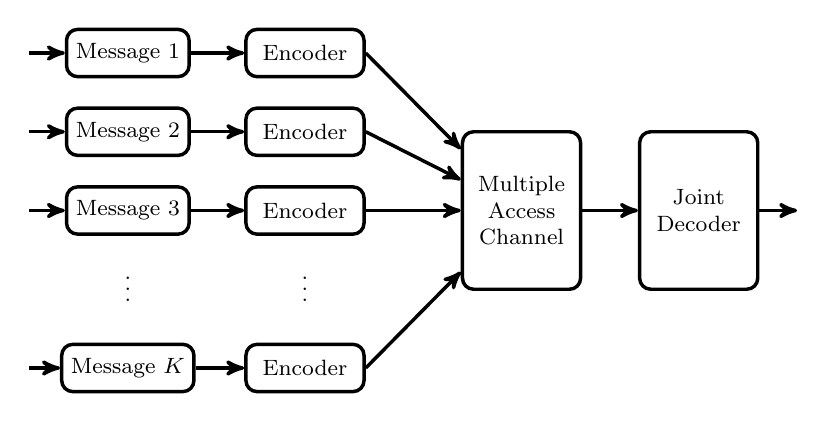
\begin{tikzpicture}
  [
  font=\footnotesize, draw=black, >=stealth', line width=1.25pt,
  channel/.style={rectangle, minimum height=20mm, minimum width=15mm, draw=black, rounded corners},
  encoder/.style={rectangle, minimum height=6mm, minimum width=15mm, draw=black, rounded corners},
  decoder/.style={rectangle, minimum height=20mm, minimum width=15mm, draw=black, rounded corners},
  message/.style={rectangle, minimum height=6mm, minimum width=15mm, draw=black, rounded corners}
  ]

\foreach \e in {1,2,3,5} {
  \node[encoder] (e\e) at (2.25,3-\e) {Encoder};
}

\foreach \m in {1,2,3} {
  \node[message] (m\m) at (0.0,3-\m) {Message~${\m}$}
  edge[->] (e\m);
  \draw[<-] (m\m) -- (-1.25,3-\m);
}

\foreach \m in {5} {
  \node[message] (m\m) at (0.0,3-\m) {Message~$K$}
  edge[->] (e\m);
  \draw[<-] (m\m) -- (-1.25,3-\m);
}

\node at (0,-0.9) {$\vdots$};
\node at (2.25,-0.9) {$\vdots$};

\node[channel,align=center] (channel) at (5,0) {Multiple\\Access\\Channel};
\node[decoder,align=center] (decoder) at (7.25,0) {Joint\\Decoder};
\draw[->] (channel) -- (decoder);

\draw[->] (decoder.east) -- (8.5,0);

\draw[->] (e1.east) -- (channel);
\draw[->] (e2.east) -- (channel);
\draw[->] (e3.east) -- (channel);
\draw[->] (e5.east) -- (channel);

\end{tikzpicture}
 \end{center}
% % % % %
\vfill
% % % % %
\begin{block}{Characteristics of URA framework}
\begin{itemize}
  \item $K$ active devices, each with a $B$-bit message
  \item Multiple access channel
\end{itemize}
\end{block}
\end{frame}

% % % % % % % % % % % % % % % % % % % %

\begin{frame} \frametitle{Unsourced Random Access -- Encoding Function}
\begin{center} 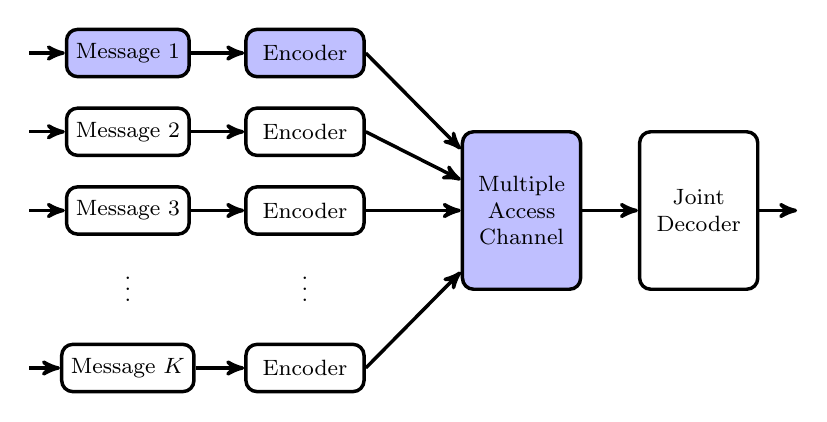
\begin{tikzpicture}
  [
  font=\footnotesize, draw=black, >=stealth', line width=1.25pt,
  channel/.style={rectangle, minimum height=20mm, minimum width=15mm, draw=black, rounded corners},
  encoder/.style={rectangle, minimum height=6mm, minimum width=15mm, draw=black, rounded corners},
  decoder/.style={rectangle, minimum height=20mm, minimum width=15mm, draw=black, rounded corners},
  message/.style={rectangle, minimum height=6mm, minimum width=15mm, draw=black, rounded corners}
  ]

\node[encoder, fill=blue!25] (e1) at (2.25,2) {Encoder};
\foreach \e in {2,3,5} {
  \node[encoder] (e\e) at (2.25,3-\e) {Encoder};
}

\node[message, fill=blue!25] (m1) at (0.0,2) {Message~$1$}
edge[->] (e1);
\draw[<-] (m1) -- (-1.25,2);
\foreach \m in {2,3} {
  \node[message] (m\m) at (0.0,3-\m) {Message~${\m}$}
  edge[->] (e\m);
  \draw[<-] (m\m) -- (-1.25,3-\m);
}

\foreach \m in {5} {
  \node[message] (m\m) at (0.0,3-\m) {Message~$K$}
  edge[->] (e\m);
  \draw[<-] (m\m) -- (-1.25,3-\m);
}

\node at (0,-0.9) {$\vdots$};
\node at (2.25,-0.9) {$\vdots$};

\node[channel,align=center,fill=blue!25] (channel) at (5,0) {Multiple\\Access\\Channel};
\node[decoder,align=center] (decoder) at (7.25,0) {Joint\\Decoder};
\draw[->] (channel) -- (decoder);

\draw[->] (decoder.east) -- (8.5,0);

\draw[->] (e1.east) -- (channel);
\draw[->] (e2.east) -- (channel);
\draw[->] (e3.east) -- (channel);
\draw[->] (e5.east) -- (channel);

\end{tikzpicture}
 \end{center}
% % % % %
\vfill
% % % % %
\begin{block}{Characteristics of URA framework}
\begin{itemize}
  \item Every device employs the same encoder $f: \{ 0, 1 \}^B \rightarrow \mathbb{R}^n$
  \item Decoder must produce an unordered list of messages
\end{itemize}
\end{block}
\end{frame}

% % % % % % % % % % % % % % % % % % % %

\begin{frame} \frametitle{Unsourced Random Access -- Encoding Function}
\begin{center} \input{Figures-URA/signaldictionary1a} \end{center}
\end{frame}

% % % % % % % % % % % % % % % % % % % %

\begin{frame} \frametitle{Unsourced Random Access -- Encoding Function}
\begin{center} \input{Figures-URA/signaldictionary1b} \end{center}
\end{frame}

% % % % % % % % % % % % % % % % % % % %

\begin{frame} \frametitle{Unsourced Random Access -- Encoding Function}
\begin{center} \input{Figures-URA/signaldictionary1c} \end{center}
\end{frame}

% % % % % % % % % % % % % % % % % % % %

\begin{frame} \frametitle{Unsourced Random Access -- Encoding Function}
\begin{center} \input{Figures-URA/signaldictionary1d} \end{center}
\end{frame}

% % % % % % % % % % % % % % % % % % % %

\begin{frame} \frametitle{Unsourced Random Access -- Encoding Function}
\begin{center} \begin{tikzpicture}
[draw=black, line width=0.75pt,>=stealth',
entry/.style={rectangle, draw, inner sep=0pt, minimum size=2.5mm},
symbol/.style={rectangle, draw, opacity=0, inner sep=0pt, minimum size=2.5mm}]

\node[entry, fill=blue!57] (x0y0) at (0.0,0.0) {};
\node[entry, fill=blue!71] (x0y1) at (0.0,0.25) {};
\node[entry, fill=blue!99] (x0y2) at (0.0,0.5) {};
\node[entry, fill=blue!59] (x0y3) at (0.0,0.75) {};
\node[entry, fill=blue!57] (x0y4) at (0.0,1.0) {};
\node[entry, fill=blue!65] (x0y5) at (0.0,1.25) {};
\node[entry, fill=blue!75] (x0y6) at (0.0,1.5) {};
\node[entry, fill=blue!24] (x0y7) at (0.0,1.75) {};
\node[entry, fill=blue!23] (x0y8) at (0.0,2.0) {};
\node[entry, fill=blue!65] (x0y9) at (0.0,2.25) {};
\node[entry, fill=blue!60] (x0y10) at (0.0,2.5) {};
\node[entry, fill=blue!80] (x0y11) at (0.0,2.75) {};

\node[entry, fill=blue!78] (x1y0) at (0.25,0.0) {};
\node[entry, fill=blue!101] (x1y1) at (0.25,0.25) {};
\node[entry, fill=blue!23] (x1y2) at (0.25,0.5) {};
\node[entry, fill=blue!12] (x1y3) at (0.25,0.75) {};
\node[entry, fill=blue!57] (x1y4) at (0.25,1.0) {};
\node[entry, fill=blue!38] (x1y5) at (0.25,1.25) {};
\node[entry, fill=blue!18] (x1y6) at (0.25,1.5) {};
\node[entry, fill=blue!11] (x1y7) at (0.25,1.75) {};
\node[entry, fill=blue!68] (x1y8) at (0.25,2.0) {};
\node[entry, fill=blue!88] (x1y9) at (0.25,2.25) {};
\node[entry, fill=blue!81] (x1y10) at (0.25,2.5) {};
\node[entry, fill=blue!5] (x1y11) at (0.25,2.75) {};

\node[entry, fill=blue!76] (x2y0) at (0.5,0.0) {};
\node[entry, fill=blue!50] (x2y1) at (0.5,0.25) {};
\node[entry, fill=blue!57] (x2y2) at (0.5,0.5) {};
\node[entry, fill=blue!83] (x2y3) at (0.5,0.75) {};
\node[entry, fill=blue!94] (x2y4) at (0.5,1.0) {};
\node[entry, fill=blue!78] (x2y5) at (0.5,1.25) {};
\node[entry, fill=blue!83] (x2y6) at (0.5,1.5) {};
\node[entry, fill=blue!20] (x2y7) at (0.5,1.75) {};
\node[entry, fill=blue!79] (x2y8) at (0.5,2.0) {};
\node[entry, fill=blue!1] (x2y9) at (0.5,2.25) {};
\node[entry, fill=blue!67] (x2y10) at (0.5,2.5) {};
\node[entry, fill=blue!8] (x2y11) at (0.5,2.75) {};

\node[entry, fill=blue!7] (x3y0) at (0.75,0.0) {};
\node[entry, fill=blue!4] (x3y1) at (0.75,0.25) {};
\node[entry, fill=blue!24] (x3y2) at (0.75,0.5) {};
\node[entry, fill=blue!30] (x3y3) at (0.75,0.75) {};
\node[entry, fill=blue!76] (x3y4) at (0.75,1.0) {};
\node[entry, fill=blue!3] (x3y5) at (0.75,1.25) {};
\node[entry, fill=blue!99] (x3y6) at (0.75,1.5) {};
\node[entry, fill=blue!59] (x3y7) at (0.75,1.75) {};
\node[entry, fill=blue!41] (x3y8) at (0.75,2.0) {};
\node[entry, fill=blue!56] (x3y9) at (0.75,2.25) {};
\node[entry, fill=blue!75] (x3y10) at (0.75,2.5) {};
\node[entry, fill=blue!25] (x3y11) at (0.75,2.75) {};

\node[entry, fill=blue!66] (x4y0) at (1.0,0.0) {};
\node[entry, fill=blue!29] (x4y1) at (1.0,0.25) {};
\node[entry, fill=blue!81] (x4y2) at (1.0,0.5) {};
\node[entry, fill=blue!37] (x4y3) at (1.0,0.75) {};
\node[entry, fill=blue!63] (x4y4) at (1.0,1.0) {};
\node[entry, fill=blue!0] (x4y5) at (1.0,1.25) {};
\node[entry, fill=blue!84] (x4y6) at (1.0,1.5) {};
\node[entry, fill=blue!10] (x4y7) at (1.0,1.75) {};
\node[entry, fill=blue!58] (x4y8) at (1.0,2.0) {};
\node[entry, fill=blue!83] (x4y9) at (1.0,2.25) {};
\node[entry, fill=blue!35] (x4y10) at (1.0,2.5) {};
\node[entry, fill=blue!52] (x4y11) at (1.0,2.75) {};

\node[entry, fill=blue!70] (x5y0) at (1.25,0.0) {};
\node[entry, fill=blue!10] (x5y1) at (1.25,0.25) {};
\node[entry, fill=blue!90] (x5y2) at (1.25,0.5) {};
\node[entry, fill=blue!32] (x5y3) at (1.25,0.75) {};
\node[entry, fill=blue!40] (x5y4) at (1.25,1.0) {};
\node[entry, fill=blue!97] (x5y5) at (1.25,1.25) {};
\node[entry, fill=blue!29] (x5y6) at (1.25,1.5) {};
\node[entry, fill=blue!65] (x5y7) at (1.25,1.75) {};
\node[entry, fill=blue!36] (x5y8) at (1.25,2.0) {};
\node[entry, fill=blue!3] (x5y9) at (1.25,2.25) {};
\node[entry, fill=blue!8] (x5y10) at (1.25,2.5) {};
\node[entry, fill=blue!72] (x5y11) at (1.25,2.75) {};

\node[entry, fill=blue!98] (x6y0) at (1.5,0.0) {};
\node[entry, fill=blue!13] (x6y1) at (1.5,0.25) {};
\node[entry, fill=blue!51] (x6y2) at (1.5,0.5) {};
\node[entry, fill=blue!13] (x6y3) at (1.5,0.75) {};
\node[entry, fill=blue!37] (x6y4) at (1.5,1.0) {};
\node[entry, fill=blue!49] (x6y5) at (1.5,1.25) {};
\node[entry, fill=blue!8] (x6y6) at (1.5,1.5) {};
\node[entry, fill=blue!2] (x6y7) at (1.5,1.75) {};
\node[entry, fill=blue!87] (x6y8) at (1.5,2.0) {};
\node[entry, fill=blue!0] (x6y9) at (1.5,2.25) {};
\node[entry, fill=blue!27] (x6y10) at (1.5,2.5) {};
\node[entry, fill=blue!26] (x6y11) at (1.5,2.75) {};

\node[entry, fill=blue!6] (x7y0) at (1.75,0.0) {};
\node[entry, fill=blue!60] (x7y1) at (1.75,0.25) {};
\node[entry, fill=blue!48] (x7y2) at (1.75,0.5) {};
\node[entry, fill=blue!90] (x7y3) at (1.75,0.75) {};
\node[entry, fill=blue!50] (x7y4) at (1.75,1.0) {};
\node[entry, fill=blue!53] (x7y5) at (1.75,1.25) {};
\node[entry, fill=blue!9] (x7y6) at (1.75,1.5) {};
\node[entry, fill=blue!72] (x7y7) at (1.75,1.75) {};
\node[entry, fill=blue!80] (x7y8) at (1.75,2.0) {};
\node[entry, fill=blue!25] (x7y9) at (1.75,2.25) {};
\node[entry, fill=blue!99] (x7y10) at (1.75,2.5) {};
\node[entry, fill=blue!86] (x7y11) at (1.75,2.75) {};

\node[entry, fill=blue!34] (x8y0) at (2.0,0.0) {};
\node[entry, fill=blue!43] (x8y1) at (2.0,0.25) {};
\node[entry, fill=blue!11] (x8y2) at (2.0,0.5) {};
\node[entry, fill=blue!39] (x8y3) at (2.0,0.75) {};
\node[entry, fill=blue!42] (x8y4) at (2.0,1.0) {};
\node[entry, fill=blue!1] (x8y5) at (2.0,1.25) {};
\node[entry, fill=blue!52] (x8y6) at (2.0,1.5) {};
\node[entry, fill=blue!97] (x8y7) at (2.0,1.75) {};
\node[entry, fill=blue!15] (x8y8) at (2.0,2.0) {};
\node[entry, fill=blue!17] (x8y9) at (2.0,2.25) {};
\node[entry, fill=blue!31] (x8y10) at (2.0,2.5) {};
\node[entry, fill=blue!90] (x8y11) at (2.0,2.75) {};

\node[entry, fill=blue!12] (x9y0) at (2.25,0.0) {};
\node[entry, fill=blue!1] (x9y1) at (2.25,0.25) {};
\node[entry, fill=blue!7] (x9y2) at (2.25,0.5) {};
\node[entry, fill=blue!59] (x9y3) at (2.25,0.75) {};
\node[entry, fill=blue!62] (x9y4) at (2.25,1.0) {};
\node[entry, fill=blue!22] (x9y5) at (2.25,1.25) {};
\node[entry, fill=blue!87] (x9y6) at (2.25,1.5) {};
\node[entry, fill=blue!71] (x9y7) at (2.25,1.75) {};
\node[entry, fill=blue!24] (x9y8) at (2.25,2.0) {};
\node[entry, fill=blue!57] (x9y9) at (2.25,2.25) {};
\node[entry, fill=blue!65] (x9y10) at (2.25,2.5) {};
\node[entry, fill=blue!24] (x9y11) at (2.25,2.75) {};

\node[entry, fill=blue!93] (x10y0) at (2.5,0.0) {};
\node[entry, fill=blue!98] (x10y1) at (2.5,0.25) {};
\node[entry, fill=blue!16] (x10y2) at (2.5,0.5) {};
\node[entry, fill=blue!53] (x10y3) at (2.5,0.75) {};
\node[entry, fill=blue!82] (x10y4) at (2.5,1.0) {};
\node[entry, fill=blue!49] (x10y5) at (2.5,1.25) {};
\node[entry, fill=blue!14] (x10y6) at (2.5,1.5) {};
\node[entry, fill=blue!50] (x10y7) at (2.5,1.75) {};
\node[entry, fill=blue!53] (x10y8) at (2.5,2.0) {};
\node[entry, fill=blue!27] (x10y9) at (2.5,2.25) {};
\node[entry, fill=blue!0] (x10y10) at (2.5,2.5) {};
\node[entry, fill=blue!34] (x10y11) at (2.5,2.75) {};

\node[entry, fill=blue!75] (x11y0) at (2.75,0.0) {};
\node[entry, fill=blue!38] (x11y1) at (2.75,0.25) {};
\node[entry, fill=blue!2] (x11y2) at (2.75,0.5) {};
\node[entry, fill=blue!26] (x11y3) at (2.75,0.75) {};
\node[entry, fill=blue!23] (x11y4) at (2.75,1.0) {};
\node[entry, fill=blue!50] (x11y5) at (2.75,1.25) {};
\node[entry, fill=blue!77] (x11y6) at (2.75,1.5) {};
\node[entry, fill=blue!82] (x11y7) at (2.75,1.75) {};
\node[entry, fill=blue!73] (x11y8) at (2.75,2.0) {};
\node[entry, fill=blue!12] (x11y9) at (2.75,2.25) {};
\node[entry, fill=blue!5] (x11y10) at (2.75,2.5) {};
\node[entry, fill=blue!18] (x11y11) at (2.75,2.75) {};

\node[entry, fill=blue!27] (x12y0) at (3.0,0.0) {};
\node[entry, fill=blue!56] (x12y1) at (3.0,0.25) {};
\node[entry, fill=blue!33] (x12y2) at (3.0,0.5) {};
\node[entry, fill=blue!1] (x12y3) at (3.0,0.75) {};
\node[entry, fill=blue!98] (x12y4) at (3.0,1.0) {};
\node[entry, fill=blue!78] (x12y5) at (3.0,1.25) {};
\node[entry, fill=blue!42] (x12y6) at (3.0,1.5) {};
\node[entry, fill=blue!37] (x12y7) at (3.0,1.75) {};
\node[entry, fill=blue!49] (x12y8) at (3.0,2.0) {};
\node[entry, fill=blue!9] (x12y9) at (3.0,2.25) {};
\node[entry, fill=blue!9] (x12y10) at (3.0,2.5) {};
\node[entry, fill=blue!11] (x12y11) at (3.0,2.75) {};

\node[entry, fill=blue!26] (x13y0) at (3.25,0.0) {};
\node[entry, fill=blue!74] (x13y1) at (3.25,0.25) {};
\node[entry, fill=blue!81] (x13y2) at (3.25,0.5) {};
\node[entry, fill=blue!31] (x13y3) at (3.25,0.75) {};
\node[entry, fill=blue!1] (x13y4) at (3.25,1.0) {};
\node[entry, fill=blue!76] (x13y5) at (3.25,1.25) {};
\node[entry, fill=blue!47] (x13y6) at (3.25,1.5) {};
\node[entry, fill=blue!47] (x13y7) at (3.25,1.75) {};
\node[entry, fill=blue!79] (x13y8) at (3.25,2.0) {};
\node[entry, fill=blue!58] (x13y9) at (3.25,2.25) {};
\node[entry, fill=blue!16] (x13y10) at (3.25,2.5) {};
\node[entry, fill=blue!75] (x13y11) at (3.25,2.75) {};

\node[entry, fill=blue!61] (x14y0) at (3.5,0.0) {};
\node[entry, fill=blue!73] (x14y1) at (3.5,0.25) {};
\node[entry, fill=blue!17] (x14y2) at (3.5,0.5) {};
\node[entry, fill=blue!49] (x14y3) at (3.5,0.75) {};
\node[entry, fill=blue!23] (x14y4) at (3.5,1.0) {};
\node[entry, fill=blue!80] (x14y5) at (3.5,1.25) {};
\node[entry, fill=blue!19] (x14y6) at (3.5,1.5) {};
\node[entry, fill=blue!39] (x14y7) at (3.5,1.75) {};
\node[entry, fill=blue!29] (x14y8) at (3.5,2.0) {};
\node[entry, fill=blue!78] (x14y9) at (3.5,2.25) {};
\node[entry, fill=blue!31] (x14y10) at (3.5,2.5) {};
\node[entry, fill=blue!92] (x14y11) at (3.5,2.75) {};

\node[entry, fill=blue!24] (x15y0) at (3.75,0.0) {};
\node[entry, fill=blue!20] (x15y1) at (3.75,0.25) {};
\node[entry, fill=blue!94] (x15y2) at (3.75,0.5) {};
\node[entry, fill=blue!80] (x15y3) at (3.75,0.75) {};
\node[entry, fill=blue!70] (x15y4) at (3.75,1.0) {};
\node[entry, fill=blue!25] (x15y5) at (3.75,1.25) {};
\node[entry, fill=blue!87] (x15y6) at (3.75,1.5) {};
\node[entry, fill=blue!49] (x15y7) at (3.75,1.75) {};
\node[entry, fill=blue!61] (x15y8) at (3.75,2.0) {};
\node[entry, fill=blue!77] (x15y9) at (3.75,2.25) {};
\node[entry, fill=blue!10] (x15y10) at (3.75,2.5) {};
\node[entry, fill=blue!53] (x15y11) at (3.75,2.75) {};

\node[entry, fill=blue!6] (x16y0) at (4.0,0.0) {};
\node[entry, fill=blue!13] (x16y1) at (4.0,0.25) {};
\node[entry, fill=blue!13] (x16y2) at (4.0,0.5) {};
\node[entry, fill=blue!4] (x16y3) at (4.0,0.75) {};
\node[entry, fill=blue!65] (x16y4) at (4.0,1.0) {};
\node[entry, fill=blue!32] (x16y5) at (4.0,1.25) {};
\node[entry, fill=blue!30] (x16y6) at (4.0,1.5) {};
\node[entry, fill=blue!94] (x16y7) at (4.0,1.75) {};
\node[entry, fill=blue!90] (x16y8) at (4.0,2.0) {};
\node[entry, fill=blue!50] (x16y9) at (4.0,2.25) {};
\node[entry, fill=blue!32] (x16y10) at (4.0,2.5) {};
\node[entry, fill=blue!53] (x16y11) at (4.0,2.75) {};

\node[entry, fill=blue!76] (x17y0) at (4.25,0.0) {};
\node[entry, fill=blue!62] (x17y1) at (4.25,0.25) {};
\node[entry, fill=blue!37] (x17y2) at (4.25,0.5) {};
\node[entry, fill=blue!66] (x17y3) at (4.25,0.75) {};
\node[entry, fill=blue!22] (x17y4) at (4.25,1.0) {};
\node[entry, fill=blue!92] (x17y5) at (4.25,1.25) {};
\node[entry, fill=blue!8] (x17y6) at (4.25,1.5) {};
\node[entry, fill=blue!16] (x17y7) at (4.25,1.75) {};
\node[entry, fill=blue!29] (x17y8) at (4.25,2.0) {};
\node[entry, fill=blue!61] (x17y9) at (4.25,2.25) {};
\node[entry, fill=blue!71] (x17y10) at (4.25,2.5) {};
\node[entry, fill=blue!83] (x17y11) at (4.25,2.75) {};

\node[entry, fill=blue!78] (x18y0) at (4.5,0.0) {};
\node[entry, fill=blue!78] (x18y1) at (4.5,0.25) {};
\node[entry, fill=blue!9] (x18y2) at (4.5,0.5) {};
\node[entry, fill=blue!35] (x18y3) at (4.5,0.75) {};
\node[entry, fill=blue!27] (x18y4) at (4.5,1.0) {};
\node[entry, fill=blue!26] (x18y5) at (4.5,1.25) {};
\node[entry, fill=blue!95] (x18y6) at (4.5,1.5) {};
\node[entry, fill=blue!2] (x18y7) at (4.5,1.75) {};
\node[entry, fill=blue!8] (x18y8) at (4.5,2.0) {};
\node[entry, fill=blue!34] (x18y9) at (4.5,2.25) {};
\node[entry, fill=blue!52] (x18y10) at (4.5,2.5) {};
\node[entry, fill=blue!57] (x18y11) at (4.5,2.75) {};

\node[entry, fill=blue!31] (x19y0) at (4.75,0.0) {};
\node[entry, fill=blue!7] (x19y1) at (4.75,0.25) {};
\node[entry, fill=blue!5] (x19y2) at (4.75,0.5) {};
\node[entry, fill=blue!22] (x19y3) at (4.75,0.75) {};
\node[entry, fill=blue!36] (x19y4) at (4.75,1.0) {};
\node[entry, fill=blue!47] (x19y5) at (4.75,1.25) {};
\node[entry, fill=blue!67] (x19y6) at (4.75,1.5) {};
\node[entry, fill=blue!73] (x19y7) at (4.75,1.75) {};
\node[entry, fill=blue!16] (x19y8) at (4.75,2.0) {};
\node[entry, fill=blue!11] (x19y9) at (4.75,2.25) {};
\node[entry, fill=blue!46] (x19y10) at (4.75,2.5) {};
\node[entry, fill=blue!17] (x19y11) at (4.75,2.75) {};

\node[entry, fill=blue!57] (x20y0) at (5.0,0.0) {};
\node[entry, fill=blue!42] (x20y1) at (5.0,0.25) {};
\node[entry, fill=blue!84] (x20y2) at (5.0,0.5) {};
\node[entry, fill=blue!93] (x20y3) at (5.0,0.75) {};
\node[entry, fill=blue!88] (x20y4) at (5.0,1.0) {};
\node[entry, fill=blue!66] (x20y5) at (5.0,1.25) {};
\node[entry, fill=blue!74] (x20y6) at (5.0,1.5) {};
\node[entry, fill=blue!17] (x20y7) at (5.0,1.75) {};
\node[entry, fill=blue!75] (x20y8) at (5.0,2.0) {};
\node[entry, fill=blue!4] (x20y9) at (5.0,2.25) {};
\node[entry, fill=blue!2] (x20y10) at (5.0,2.5) {};
\node[entry, fill=blue!60] (x20y11) at (5.0,2.75) {};

\node[entry, fill=blue!45] (x21y0) at (5.25,0.0) {};
\node[entry, fill=blue!89] (x21y1) at (5.25,0.25) {};
\node[entry, fill=blue!39] (x21y2) at (5.25,0.5) {};
\node[entry, fill=blue!4] (x21y3) at (5.25,0.75) {};
\node[entry, fill=blue!2] (x21y4) at (5.25,1.0) {};
\node[entry, fill=blue!76] (x21y5) at (5.25,1.25) {};
\node[entry, fill=blue!81] (x21y6) at (5.25,1.5) {};
\node[entry, fill=blue!9] (x21y7) at (5.25,1.75) {};
\node[entry, fill=blue!61] (x21y8) at (5.25,2.0) {};
\node[entry, fill=blue!8] (x21y9) at (5.25,2.25) {};
\node[entry, fill=blue!93] (x21y10) at (5.25,2.5) {};
\node[entry, fill=blue!39] (x21y11) at (5.25,2.75) {};

\node[entry, fill=blue!40] (x22y0) at (5.5,0.0) {};
\node[entry, fill=blue!17] (x22y1) at (5.5,0.25) {};
\node[entry, fill=blue!9] (x22y2) at (5.5,0.5) {};
\node[entry, fill=blue!9] (x22y3) at (5.5,0.75) {};
\node[entry, fill=blue!57] (x22y4) at (5.5,1.0) {};
\node[entry, fill=blue!69] (x22y5) at (5.5,1.25) {};
\node[entry, fill=blue!47] (x22y6) at (5.5,1.5) {};
\node[entry, fill=blue!94] (x22y7) at (5.5,1.75) {};
\node[entry, fill=blue!5] (x22y8) at (5.5,2.0) {};
\node[entry, fill=blue!94] (x22y9) at (5.5,2.25) {};
\node[entry, fill=blue!94] (x22y10) at (5.5,2.5) {};
\node[entry, fill=blue!90] (x22y11) at (5.5,2.75) {};

\node[entry, fill=blue!16] (x23y0) at (5.75,0.0) {};
\node[entry, fill=blue!101] (x23y1) at (5.75,0.25) {};
\node[entry, fill=blue!43] (x23y2) at (5.75,0.5) {};
\node[entry, fill=blue!45] (x23y3) at (5.75,0.75) {};
\node[entry, fill=blue!10] (x23y4) at (5.75,1.0) {};
\node[entry, fill=blue!87] (x23y5) at (5.75,1.25) {};
\node[entry, fill=blue!60] (x23y6) at (5.75,1.5) {};
\node[entry, fill=blue!9] (x23y7) at (5.75,1.75) {};
\node[entry, fill=blue!53] (x23y8) at (5.75,2.0) {};
\node[entry, fill=blue!101] (x23y9) at (5.75,2.25) {};
\node[entry, fill=blue!3] (x23y10) at (5.75,2.5) {};
\node[entry, fill=blue!63] (x23y11) at (5.75,2.75) {};

\node[symbol] (s01) at (6.5,-3.00) {};
\node[symbol] (s02) at (6.5,-2.75) {};
\node[symbol] (s03) at (6.5,-2.50) {};
\node[symbol] (s04) at (6.5,-2.25) {};
\node[symbol] (s05) at (6.5,-2.00) {};
\node[symbol] (s06) at (6.5,-1.75) {};
\node[symbol] (s07) at (6.5,-1.50) {};
\node[symbol] (s08) at (6.5,-1.25) {};
\node[symbol] (s09) at (6.5,-1.00) {};
\node[symbol] (s10) at (6.5,-0.75) {};
\node[symbol] (s11) at (6.5,-0.50) {};
\node[symbol] (s12) at (6.5,-0.25) {};
\node[symbol] (s13) at (6.5,0) {};
\node[symbol] (s14) at (6.5,0.25) {};
\node[symbol] (s15) at (6.5,0.50) {};
\node[symbol] (s16) at (6.5,0.75) {};
\node[symbol] (s17) at (6.5,1.00) {};
\node[symbol] (s18) at (6.5,1.25) {};
\node[symbol] (s19) at (6.5,1.50) {};
\node[symbol] (s20) at (6.5,1.75) {};
\node[symbol] (s21) at (6.5,2.00) {};
\node[symbol] (s22) at (6.5,2.25) {};
\node[symbol] (s23) at (6.5,2.50) {};
\node[symbol] (s24) at (6.5,2.75) {};

\draw[|-|,opacity=0] (-0.125, 3.125) to node[above] {\small Signal dictionary} (5.875, 3.125);
\draw[<-] (-0.375, -0.125) to node[above,rotate=90] {\small Time} (-0.375, 2.875);
\draw[|-|,opacity=0] (6.875, -3.125) to node[above,rotate=-90] {\small Message index} (6.875, 2.875);

\node (suB) at (2.875, 3.25) {\small Single user with message $11111$};
\node (fB) at (7.25, 1.375) {\small $f(11111)$};
\draw[->] (fB) to (6,1.375);

\node[text width=5cm] (equation) at (3.875, -1.625) {Message Encoding:
\[ \begin{split} &f: \{ 0, 1 \}^B \mapsto \mathbb{R}^n \\
&f(\text{binary message}) = \text{signal} \end{split} \]};

\end{tikzpicture}
 \end{center}
\end{frame}

% % % % % % % % % % % % % % % % % % % %

\begin{frame} \frametitle{Unsourced Random Access -- Encoding Function}
\begin{center} \input{Figures-URA/signaldictionary1} \end{center}
\end{frame}

% % % % % % % % % % % % % % % % % % % %

\begin{frame} \frametitle{Unsourced Random Access -- Index Representation}
\begin{center} \input{Figures-URA/signaldictionary1i} \end{center}
\end{frame}

% % % % % % % % % % % % % % % % % % % %

\begin{frame} \frametitle{Unsourced Random Access -- Index Representation}
\begin{center} \input{Figures-URA/signaldictionary1j} \end{center}
\end{frame}

% % % % % % % % % % % % % % % % % % % %

\begin{frame}
\frametitle{Unsourced Random Access -- CS Analogy}
% % % % %
\hfill
\scalebox{0.75}{\input{Figures-URA/compressedura}}
\vspace{-2cm}
% % % % %
\begin{columns}
\column{.80\textwidth}
\scalebox{0.8}{\input{Figures-URA/URA2}}
\column{.15\textwidth}
\end{columns}
% % % % %
\end{frame}

% % % % % % % % % % % % % % % % % % % %

\begin{frame}
\frametitle{Abstract CS Challenge}
% % % % %
\begin{columns}
\column{0.54\textwidth}
\structure{\large Problem setting}
  \begin{itemize}
  \item Noisy compressed sensing
  \begin{equation*}
  \yv = \boldsymbol{\Phi} \sv + \zv
  \end{equation*}
  where $\sv$ is $K$ sparse
  \item $\sv$ has non-negative integer entries
  \item $\boldsymbol{\Phi}.\mathtt{shape} \approx 32,768 \times 2^{128}$
  \item $\zv$ is additive Gaussian noise
  \end{itemize}
\column{0.44\textwidth}
  \hspace{-1cm} \scalebox{0.75}{\input{Figures-URA/compressedura1}}
\end{columns}
% % % % %
\vfill
% % % % %
\begin{block}{Performance evaluation}
  \begin{itemize}
  \item Number of mistakes in support recovery normalized by $K$
  \item Related to the per user probability of error in MAC setting
  \end{itemize}
\end{block}
\end{frame}

% % % % % % % % % % % % % % % % % % % %

\begin{frame}
\frametitle{Abstract CS Challenge}
% % % % %
\begin{columns}
\column{0.54\textwidth}
\structure{\large Problem setting}
  \begin{itemize}
  \item Noisy compressed sensing
  \begin{equation*}
  \yv = \boldsymbol{\Phi} \sv + \zv
  \end{equation*}
  where $\sv$ is $K$ sparse
  \item $\sv$ has non-negative integer entries
  \item $\boldsymbol{\Phi}.\mathtt{shape} \approx 32,768 \times 2^{128}$
  \item $\zv$ is additive Gaussian noise
  \end{itemize}
\column{0.44\textwidth}
  \hspace{-1cm} \scalebox{0.75}{\input{Figures-URA/compressedura1}}
\end{columns}
% % % % %
\vfill
% % % % %
\begin{alertblock}{Practical issue}
  \begin{itemize}
  \item Width of sensing matrix is huge
  \item Existing CS solvers will not execute at that scale
  \end{itemize}
\end{alertblock}
\end{frame}

% % % % % % % % % % % % % % % % % % % %

\begin{frame} \frametitle{Matrix Width \& Sparsity Undersampling Tradeoff}
\begin{center} \input{Figures-URA/pnas1} \end{center}
% % % % %
\begin{columns}
\column{0.48\textwidth}
\begin{itemize}
\item Undersampling fraction \[ \delta = \frac{32,768}{2^{128}} = 2^{-113} \]
\end{itemize}
\column{0.48\textwidth}
\begin{itemize}
\item Measure of sparsity \[ \rho = \frac{256}{32,768} = 2^{-7} \]
\end{itemize}
\end{columns}
% % % % %
\end{frame}

% % % % % % % % % % % % % % % % % % % %

\begin{frame}
\frametitle{Time-Division Unsourced Random Access}
% % % % %
\begin{columns}
\column{0.54\textwidth}
\structure{\large Slot partitioning}
  \begin{itemize}
  \item Observations become
  \begin{equation*}
  \yv_{\ell} = \boldsymbol{\Phi}_{\ell} \sv_{\ell} + \zv_{\ell}
  \end{equation*}
  where $\ell$ is slot label
  \item Device gets slot based on message
  \item Channel uses divided among slots
  \end{itemize}
\column{0.44\textwidth}
  \hspace{-1cm} \scalebox{0.75}{\input{Figures-URA/compressedura1a}}
\end{columns}
% % % % %
\vfill
% % % % %
\begin{alertblock}{Drawbacks}
  \begin{itemize}
  \item Matrices remain wide $2^{128}/L$
  \item Devices assigned randomly within slots
  \end{itemize}
\end{alertblock}
\end{frame}

% % % % % % % % % % % % % % % % % % % %

\begin{frame}
\frametitle{Classical Coding Techniques}
% % % % %
\begin{columns}
\column{0.54\textwidth}
\structure{\large Multi-User Coding}
  \begin{itemize}
  \item Matrix becomes codebooks
  \begin{equation*}
  \yv = \boldsymbol{\Phi}_1 \sv_1 + \boldsymbol{\Phi}_2 \sv_2 + \zv
  \end{equation*}
  \item Device picks code based on bits
  \item Well-studied for single user
  \item Fast decoding for large dictionary
  \end{itemize}
\column{0.44\textwidth}
  \hspace{-1cm} \scalebox{0.75}{\input{Figures-URA/compressedura1b}}
\end{columns}
% % % % %
\vfill
% % % % %
\begin{alertblock}{Drawbacks}
  \begin{itemize}
  \item Low complexity joint multi-user decoders are not available
  \item Devices may collide within codebook selection
  \end{itemize}
\end{alertblock}
\end{frame}

% % % % % % % % % % % % % % % % % % % %

\begin{frame}
\frametitle{Data Fragmentation}
% % % % %
\begin{center}
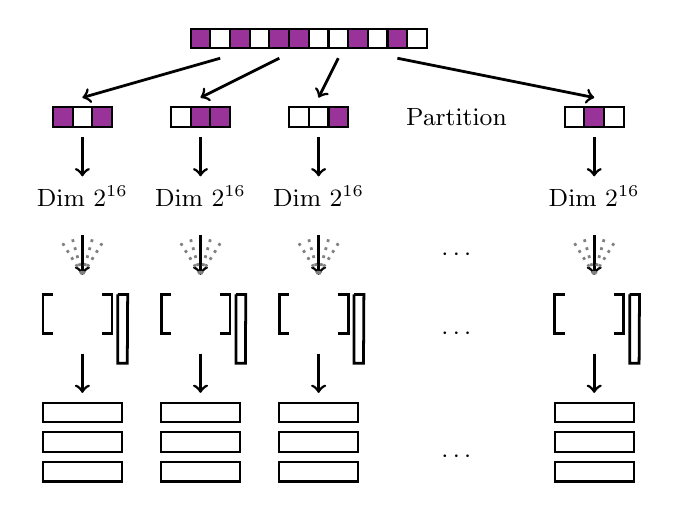
\begin{tikzpicture}
[font=\small, draw=black, line width=0.75pt,
sub0/.style={rectangle, draw, inner sep=0pt, minimum width=10mm, minimum height=2.5mm},
parity/.style={rectangle, draw, fill=cyan, inner sep=0pt, minimum size=2.5mm},
bit0/.style={rectangle, draw, inner sep=0pt, minimum size=2.5mm},
bit1/.style={rectangle, draw, fill=violet!80, inner sep=0pt, minimum size=2.5mm}]

\node[bit1] (bit0) at (0.50,8.25) {};
\node[bit0] (bit1) at (0.75,8.25) {};
\node[bit1] (bit2) at (1.00,8.25) {};
\node[bit0] (bit3) at (1.25,8.25) {};
\node[bit1] (bit4) at (1.50,8.25) {};
\node[bit1] (bit5) at (1.75,8.25) {};
\node[bit0] (bit6) at (2.00,8.25) {};
\node[bit0] (bit7) at (2.25,8.25) {};
\node[bit1] (bit8) at (2.50,8.25) {};
\node[bit0] (bit9) at (2.75,8.25) {};
\node[bit1] (bit10) at (3.00,8.25) {};
\node[bit0] (bit11) at (3.25,8.25) {};

\draw[->, line width=1pt]  (0.75,8.00) -- (-1.00,7.50);
\draw[->, line width=1pt]  (1.50,8.00) -- (0.50,7.50);
\draw[->, line width=1pt]  (2.25,8.00) -- (2.00,7.50);
\draw[->, line width=1pt]  (3.00,8.00) -- (5.50,7.50);
\node (partition) at (3.75,7.25) {Partition};

\node[bit1] (s00) at (-1.25,7.25) {};
\node[bit0] (s01) at (-1.00,7.25) {};
\node[bit1] (s02) at (-0.75,7.25) {};

\node[bit0] (s03) at (0.25,7.25) {};
\node[bit1] (s04) at (0.50,7.25) {};
\node[bit1] (s05) at (0.75,7.25) {};

\node[bit0] (s06) at (1.75,7.25) {};
\node[bit0] (s07) at (2.00,7.25) {};
\node[bit1] (s08) at (2.25,7.25) {};

\node[bit0] (s09) at (5.25,7.25) {};
\node[bit1] (s10) at (5.50,7.25) {};
\node[bit0] (s11) at (5.75,7.25) {};

\draw[->, line width=1pt]  (-1.00,7) -- (-1.00,6.5);
\draw[->, line width=1pt]  (0.50,7) -- (0.50,6.5);
\draw[->, line width=1pt]  (2.00,7) -- (2.00,6.5);
\draw[->, line width=1pt]  (5.50,7) -- (5.50,6.5);

\node (cs1) at (-1.00,6.25) {Dim~$2^{16}$};
\node (cs2) at (0.50,6.25) {Dim~$2^{16}$};
\node (cs3) at (2.00,6.25) {Dim~$2^{16}$};
\node (cs4) at (5.50,6.25) {Dim~$2^{16}$};

\foreach \v in {-1.00,0.50,2.00,5.50} {
  \draw[->, line width=1pt]  (\v,4.25) -- (\v,3.75);
  \draw[->, line width=1pt]  (\v,5.75) -- (\v,5.25);
  \draw[dotted, line width=1pt, draw=gray]  (\v-0.25,5.65) -- (\v,5.25);
  \draw[dotted, line width=1pt, draw=gray]  (\v-0.125,5.7) -- (\v,5.25);
  \draw[dotted, line width=1pt, draw=gray]  (\v+0.125,5.7) -- (\v,5.25);
  \draw[dotted, line width=1pt, draw=gray]  (\v+0.25,5.65) -- (\v,5.25);
}

\node (dots1) at (3.75,5.5) {$\cdots$};

\foreach \v in {-1.00,0.50,2.00,5.50} {
  \draw[line width=1pt] (\v-0.375,5) -- (\v-0.5,5) -- (\v-0.5,4.5) -- (\v-0.375,4.5);
  \draw[line width=1pt] (\v+0.25,5) -- (\v+0.375,5) -- (\v+0.375,4.5) -- (\v+0.25,4.5);
  \draw[line width=1pt] (\v+0.45,5) -- (\v+0.45,4.125) -- (\v+0.57,4.125) -- (\v+0.575,5) -- (\v+0.45,5);
}

\node (dots2) at (3.75,4.5) {$\cdots$};
\node (dots3) at (3.75,2.9375) {$\cdots$};

\foreach \c in {3.50, 3.125, 2.75} {
  \node[sub0] (subcs0\c) at (-1.00,\c) {};
  \node[sub0] (subcs2\c) at (0.50,\c) {};
  \node[sub0] (subcs3\c) at (2.00,\c) {};
  \node[sub0] (subcsz\c) at (5.50,\c) {};
}

\end{tikzpicture}

\end{center}
% % % % %
\begin{alertblock}{Drawbacks}
  \begin{itemize}
  \item Unordered lists of fragments
  \item Need to perform disambiguation
  \end{itemize}
\end{alertblock}
\end{frame}

% % % % % % % % % % % % % % % % % % % %

\begin{frame} \frametitle{Drastic Reduction in Matrix Width}
\begin{center} 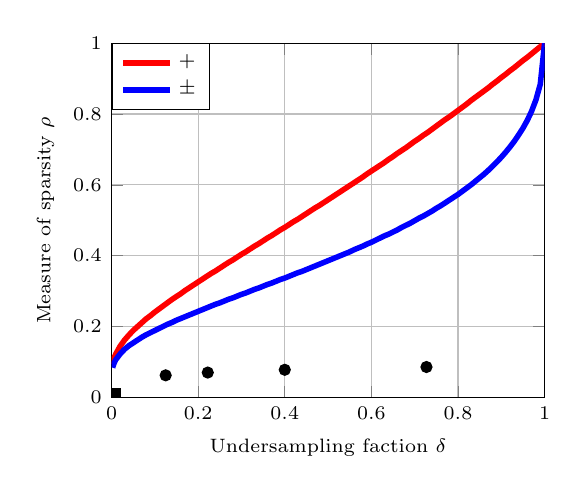
\begin{tikzpicture}

\begin{axis}[%
font=\scriptsize,
width=5.5cm,
height=4.5cm,
scale only axis,
xmin=0,
xmax=1,
xlabel={Undersampling faction $\delta$},
xmajorgrids,
ymin=0,
ymax=1,
ylabel={Measure of sparsity $\rho$},
%ylabel near ticks,
ymajorgrids,
legend style={at={(0,1)},anchor=north west,legend cell align=left,
/tikz/column 2/.style={column sep=3pt}}
]

\addplot [color=red,solid,line width=2.0pt]
  coordinates {
(0.0025,0.094) (0.005,0.107) (0.0075,0.116)
(0.01,0.123) (0.02,0.145) (0.03,0.162) (0.04,0.176) (0.05,0.189) (0.06,0.2) (0.07,0.211) (0.08,0.222) (0.09,0.231) (0.1,0.241) (0.11,0.25) (0.12,0.259) (0.13,0.268) (0.14,0.277) (0.15,0.285) (0.16,0.293) (0.17,0.302) (0.18,0.31) (0.19,0.318) (0.2,0.326) (0.21,0.334) (0.22,0.342) (0.23,0.35) (0.24,0.357) (0.25,0.365) (0.26,0.373) (0.27,0.381) (0.28,0.388) (0.29,0.396) (0.3,0.404) (0.31,0.411) (0.32,0.419) (0.33,0.427) (0.34,0.434) (0.35,0.442) (0.36,0.45) (0.37,0.457) (0.38,0.465) (0.39,0.473) (0.4,0.48) (0.41,0.488) (0.42,0.496) (0.43,0.503) (0.44,0.511) (0.45,0.519) (0.46,0.527) (0.47,0.535) (0.48,0.542) (0.49,0.55) (0.5,0.558) (0.51,0.566) (0.52,0.574) (0.53,0.582) (0.54,0.59) (0.55,0.598) (0.56,0.606) (0.57,0.614) (0.58,0.622) (0.59,0.631) (0.6,0.639) (0.61,0.647) (0.62,0.655) (0.63,0.663) (0.64,0.672) (0.65,0.68) (0.66,0.689) (0.67,0.697) (0.68,0.705) (0.69,0.714) (0.7,0.723) (0.71,0.731) (0.72,0.74) (0.73,0.748) (0.74,0.757) (0.75,0.766) (0.76,0.775) (0.77,0.784) (0.78,0.792) (0.79,0.801) (0.8,0.81) (0.81,0.819) (0.82,0.828) (0.83,0.838) (0.84,0.847) (0.85,0.856) (0.86,0.865) (0.87,0.874) (0.88,0.884) (0.89,0.893) (0.9,0.903) (0.91,0.912) (0.92,0.922) (0.93,0.931) (0.94,0.941) (0.95,0.951) (0.96,0.96) (0.97,0.97) (0.98,0.98) (0.99,0.99) (1,1)
};
\addlegendentry{$+$};

\addplot [color=blue,solid,line width=2.0pt]
  coordinates {
(0.0025,0.084) (0.005,0.094) (0.0075,0.101)
(0.01,0.107) (0.02,0.123) (0.03,0.136) (0.04,0.146) (0.05,0.154) (0.06,0.162) (0.07,0.17) (0.08,0.177) (0.09,0.183) (0.1,0.189) (0.11,0.195) (0.12,0.201) (0.13,0.207) (0.14,0.212) (0.15,0.218) (0.16,0.223) (0.17,0.228) (0.18,0.233) (0.19,0.238) (0.2,0.243) (0.21,0.248) (0.22,0.253) (0.23,0.258) (0.24,0.263) (0.25,0.267) (0.26,0.272) (0.27,0.277) (0.28,0.281) (0.29,0.286) (0.3,0.291) (0.31,0.295) (0.32,0.3) (0.33,0.305) (0.34,0.309) (0.35,0.314) (0.36,0.319) (0.37,0.323) (0.38,0.328) (0.39,0.333) (0.4,0.337) (0.41,0.342) (0.42,0.347) (0.43,0.352) (0.44,0.356) (0.45,0.361) (0.46,0.366) (0.47,0.371) (0.48,0.376) (0.49,0.381) (0.5,0.386) (0.51,0.391) (0.52,0.396) (0.53,0.401) (0.54,0.406) (0.55,0.411) (0.56,0.417) (0.57,0.422) (0.58,0.427) (0.59,0.433) (0.6,0.438) (0.61,0.444) (0.62,0.45) (0.63,0.456) (0.64,0.461) (0.65,0.467) (0.66,0.473) (0.67,0.48) (0.68,0.486) (0.69,0.492) (0.7,0.499) (0.71,0.506) (0.72,0.512) (0.73,0.519) (0.74,0.526) (0.75,0.534) (0.76,0.541) (0.77,0.549) (0.78,0.557) (0.79,0.565) (0.8,0.573) (0.81,0.582) (0.82,0.591) (0.83,0.6) (0.84,0.61) (0.85,0.62) (0.86,0.63) (0.87,0.641) (0.88,0.653) (0.89,0.665) (0.9,0.678) (0.91,0.692) (0.92,0.707) (0.93,0.723) (0.94,0.741) (0.95,0.76) (0.96,0.782) (0.97,0.808) (0.98,0.84) (0.99,0.884) (1,1)
};
\addlegendentry{$\pm$};

%\node at (axis cs: 0.2, 0.65) {Failure Region};
%\node at (axis cs: 0.685, 0.25) {Exact Reconstruction};

\filldraw [fill=black] (axis cs:0,0) rectangle (axis cs:0.02,0.025);

\filldraw (axis cs: 0.125, 0.0625) circle (2pt);
\filldraw (axis cs: 0.2222,0.0703125) circle (2pt);
\filldraw (axis cs: 0.4, 0.078125) circle (2pt);
\filldraw (axis cs: 0.7272,0.0859375) circle (2pt);

%\filldraw[color=darkgray] (axis cs: 0.000001, 0.0625) circle (1.5pt);
%\filldraw[color=darkgray] (axis cs: 0.000006, 0.0703125) circle (1.5pt);
%\filldraw[color=darkgray] (axis cs: 0.00004, 0.078125) circle (1.5pt);
%\filldraw[color=darkgray] (axis cs: 0.00018, 0.0859375) circle (1.5pt);
%\filldraw[color=darkgray] (axis cs: 0.00065, 0.09375) circle (1.5pt);
%\filldraw[color=darkgray] (axis cs: 0.00240, 0.1015625) circle (1.5pt);
%\filldraw[color=darkgray] (axis cs: 0.00446, 0.109375) circle (1.5pt);
%\filldraw[color=darkgray] (axis cs: 0.00833, 0.1171875) circle (1.5pt);
%\filldraw[color=darkgray] (axis cs: 0.03125, 0.125) circle (1.5pt);
%\filldraw[color=darkgray] (axis cs: 0.055555, 0.140625) circle (1.5pt);
%\filldraw[color=darkgray] (axis cs: 0.2, 0.15625) circle (1.5pt);
\end{axis}

\end{tikzpicture}
 \end{center}
% % % % %
\begin{columns}
\column{0.48\textwidth}
\begin{itemize}
\item Undersampling fraction \[ \delta = \frac{32,768}{L \cdot 2^{\lceil 128/L \rceil}} \]
\end{itemize}
\column{0.48\textwidth}
\begin{itemize}
\item Measure of sparsity \[ \rho = \frac{L \cdot 256}{32,768} = \frac{L}{2^7} \]
\end{itemize}
\end{columns}
% % % % %
\end{frame}

% % % % % % % % % % % % % % % % % % % %

\begin{frame}
\frametitle{Section Summary}
% % % % %
\begin{columns}
\column{0.54\textwidth}
\structure{\large Problem formulation}
  \begin{itemize}
  \item Noisy compressed sensing
  \begin{equation*}
  \yv = \boldsymbol{\Phi} \sv + \zv
  \end{equation*}
  \item URA is noisy support recovery
  \item Full control over $\boldsymbol{\Phi}$
  \item Width of sensing matrix is huge
  \item Uncoordinated access produces stochastic binning
  \end{itemize}
\column{0.44\textwidth}
  \hspace{-1cm} \scalebox{0.75}{\input{Figures-URA/compressedura1}}
\end{columns}
% % % % %
\vfill
% % % % %
\begin{block}{Possible URA design strategies}
  \begin{itemize}
  \item Sparsifying collisions
  \item Advanced coding and spreading
  \item Data fragmentation
  \end{itemize}
\end{block}
\end{frame}

% % % % % % % % % % % % % % % % % % % %


\begin{frame}
\frametitle{Pertinent References}
\begin{footnotesize}
\begin{itemize}

\item
Y.~Polyanskiy.
A perspective on massive random-access.
\emph{Proc.~Int.\ Symp.\ on Information Theory (ISIT)}, 2017.

\item
O.~Ordentlich and Y.~Polyanskiy.
Low complexity schemes for the random access Gaussian channel.
\emph{Proc.~Int.\ Symp.\ on Information Theory (ISIT)}, 2017.

\item
A.~Vem, K.~R. Narayanan, J.-F. Chamberland, and J.~Cheng.
A user-independent successive interference cancellation based coding scheme for the unsourced random access Gaussian channel.
\emph{IEEE Trans.\ on~Communications}, 2019.

\item
V.~K. Amalladinne, J.-F. Chamberland, and K.~R. Narayanan.
A coded compressed sensing scheme for unsourced multiple access.
\emph{IEEE Trans.\ on Information Theory}, 2020.

\item
R.~Calderbank and A.~Thompson.
CHIRRUP: A practical algorithm for unsourced multiple access.
\emph{Information and Inference}, December 2019.

\end{itemize}
\end{footnotesize}
\end{frame}

% % % % % % % % % % % % % % % % % % % %

\part{A Quest for Low-Complexity: \newline Coded Compressed Sensing}
\frame{\partpage}

% % % % % % % % % % % % % % % % % % % %

\begin{frame}
\frametitle{Abstract CS Challenge}
% % % % %
\begin{columns}
\column{0.54\textwidth}
\structure{\large Problem setting}
  \begin{itemize}
  \item Noisy compressed sensing
  \begin{equation*}
  \yv = \boldsymbol{\Phi} \sv + \zv
  \end{equation*}
  where $\sv$ is $K$ sparse
  \item $\sv$ has non-negative integer entries
  \item $\boldsymbol{\Phi}.\mathtt{shape} \approx 32,768 \times 2^{128}$
  \item $\zv$ is additive Gaussian noise
  \end{itemize}
\column{0.44\textwidth}
  \hspace{-1cm} \scalebox{0.75}{\input{Figures-URA/compressedura1}}
\end{columns}
% % % % %
\vfill
% % % % %
\begin{exampleblock}{Practical issue and potential direction}
  \begin{itemize}
  \item Width of sensing matrix is huge
  \item Undersampling fraction and sparsity are very small
  \end{itemize}
\end{exampleblock}
\end{frame}

% % % % % % % % % % % % % % % % % % % %

\begin{frame} \frametitle{Unsourced Random Access -- Index Representation}
\begin{center} \input{Figures-URA/signaldictionary1j} \end{center}
\end{frame}

% % % % % % % % % % % % % % % % % % % %

\begin{frame}
\frametitle{Data Fragmentation}
% % % % %
\begin{center}
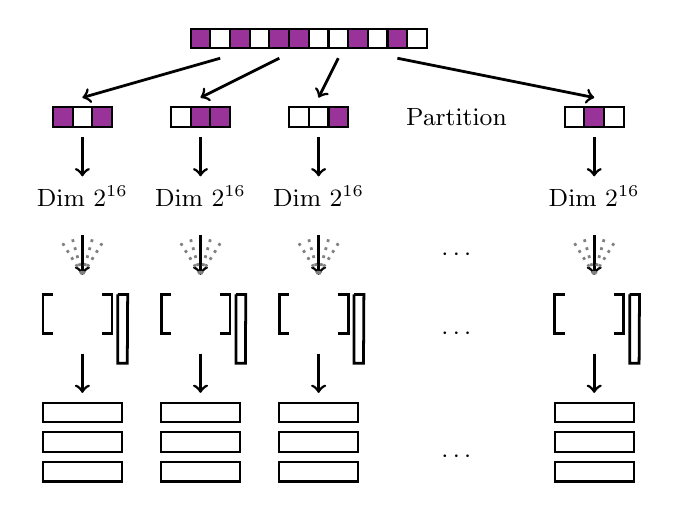
\begin{tikzpicture}
[font=\small, draw=black, line width=0.75pt,
sub0/.style={rectangle, draw, inner sep=0pt, minimum width=10mm, minimum height=2.5mm},
parity/.style={rectangle, draw, fill=cyan, inner sep=0pt, minimum size=2.5mm},
bit0/.style={rectangle, draw, inner sep=0pt, minimum size=2.5mm},
bit1/.style={rectangle, draw, fill=violet!80, inner sep=0pt, minimum size=2.5mm}]

\node[bit1] (bit0) at (0.50,8.25) {};
\node[bit0] (bit1) at (0.75,8.25) {};
\node[bit1] (bit2) at (1.00,8.25) {};
\node[bit0] (bit3) at (1.25,8.25) {};
\node[bit1] (bit4) at (1.50,8.25) {};
\node[bit1] (bit5) at (1.75,8.25) {};
\node[bit0] (bit6) at (2.00,8.25) {};
\node[bit0] (bit7) at (2.25,8.25) {};
\node[bit1] (bit8) at (2.50,8.25) {};
\node[bit0] (bit9) at (2.75,8.25) {};
\node[bit1] (bit10) at (3.00,8.25) {};
\node[bit0] (bit11) at (3.25,8.25) {};

\draw[->, line width=1pt]  (0.75,8.00) -- (-1.00,7.50);
\draw[->, line width=1pt]  (1.50,8.00) -- (0.50,7.50);
\draw[->, line width=1pt]  (2.25,8.00) -- (2.00,7.50);
\draw[->, line width=1pt]  (3.00,8.00) -- (5.50,7.50);
\node (partition) at (3.75,7.25) {Partition};

\node[bit1] (s00) at (-1.25,7.25) {};
\node[bit0] (s01) at (-1.00,7.25) {};
\node[bit1] (s02) at (-0.75,7.25) {};

\node[bit0] (s03) at (0.25,7.25) {};
\node[bit1] (s04) at (0.50,7.25) {};
\node[bit1] (s05) at (0.75,7.25) {};

\node[bit0] (s06) at (1.75,7.25) {};
\node[bit0] (s07) at (2.00,7.25) {};
\node[bit1] (s08) at (2.25,7.25) {};

\node[bit0] (s09) at (5.25,7.25) {};
\node[bit1] (s10) at (5.50,7.25) {};
\node[bit0] (s11) at (5.75,7.25) {};

\draw[->, line width=1pt]  (-1.00,7) -- (-1.00,6.5);
\draw[->, line width=1pt]  (0.50,7) -- (0.50,6.5);
\draw[->, line width=1pt]  (2.00,7) -- (2.00,6.5);
\draw[->, line width=1pt]  (5.50,7) -- (5.50,6.5);

\node (cs1) at (-1.00,6.25) {Dim~$2^{16}$};
\node (cs2) at (0.50,6.25) {Dim~$2^{16}$};
\node (cs3) at (2.00,6.25) {Dim~$2^{16}$};
\node (cs4) at (5.50,6.25) {Dim~$2^{16}$};

\foreach \v in {-1.00,0.50,2.00,5.50} {
  \draw[->, line width=1pt]  (\v,4.25) -- (\v,3.75);
  \draw[->, line width=1pt]  (\v,5.75) -- (\v,5.25);
  \draw[dotted, line width=1pt, draw=gray]  (\v-0.25,5.65) -- (\v,5.25);
  \draw[dotted, line width=1pt, draw=gray]  (\v-0.125,5.7) -- (\v,5.25);
  \draw[dotted, line width=1pt, draw=gray]  (\v+0.125,5.7) -- (\v,5.25);
  \draw[dotted, line width=1pt, draw=gray]  (\v+0.25,5.65) -- (\v,5.25);
}

\node (dots1) at (3.75,5.5) {$\cdots$};

\foreach \v in {-1.00,0.50,2.00,5.50} {
  \draw[line width=1pt] (\v-0.375,5) -- (\v-0.5,5) -- (\v-0.5,4.5) -- (\v-0.375,4.5);
  \draw[line width=1pt] (\v+0.25,5) -- (\v+0.375,5) -- (\v+0.375,4.5) -- (\v+0.25,4.5);
  \draw[line width=1pt] (\v+0.45,5) -- (\v+0.45,4.125) -- (\v+0.57,4.125) -- (\v+0.575,5) -- (\v+0.45,5);
}

\node (dots2) at (3.75,4.5) {$\cdots$};
\node (dots3) at (3.75,2.9375) {$\cdots$};

\foreach \c in {3.50, 3.125, 2.75} {
  \node[sub0] (subcs0\c) at (-1.00,\c) {};
  \node[sub0] (subcs2\c) at (0.50,\c) {};
  \node[sub0] (subcs3\c) at (2.00,\c) {};
  \node[sub0] (subcsz\c) at (5.50,\c) {};
}

\end{tikzpicture}

\end{center}
% % % % %
\begin{alertblock}{Drawbacks}
  \begin{itemize}
  \item Unordered lists of fragments
  \item Need to perform disambiguation
  \end{itemize}
\end{alertblock}
\end{frame}

% % % % % % % % % % % % % % % % % % % %

\begin{frame}
\frametitle{Fragmentation with Disambiguation}
% % % % %
\begin{center}
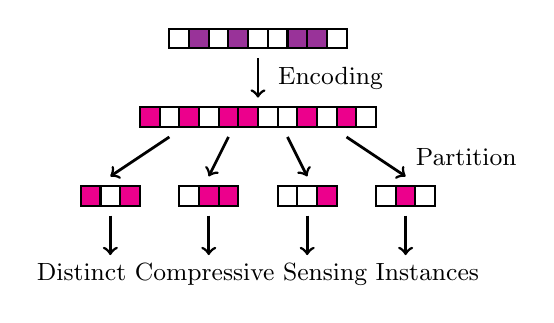
\begin{tikzpicture}
[font=\small, draw=black, line width=0.75pt,
bit0/.style={rectangle, draw, inner sep=0pt, minimum size=2.5mm},
bit1/.style={rectangle, draw, fill=violet!80, inner sep=0pt, minimum size=2.5mm},
ebit0/.style={rectangle, draw, inner sep=0pt, minimum size=2.5mm},
ebit1/.style={rectangle, draw, fill=magenta, inner sep=0pt, minimum size=2.5mm}
]

\node[bit0] (info0) at (0.875,5) {};
\node[bit1] (info1) at (1.125,5) {};
\node[bit0] (info2) at (1.375,5) {};
\node[bit1] (info3) at (1.625,5) {};
\node[bit0] (info4) at (1.875,5) {};
\node[bit0] (info5) at (2.125,5) {};
\node[bit1] (info6) at (2.375,5) {};
\node[bit1] (info7) at (2.625,5) {};
\node[bit0] (info8) at (2.875,5) {};

\draw[->, line width=1pt]  (1.875,4.75) -- (1.875,4.25);
\node[anchor=west] (coding) at (2,4.50) {Encoding};

\node[ebit1] (ebit0) at (0.50,4) {};
\node[ebit0] (ebit1) at (0.75,4) {};
\node[ebit1] (ebit2) at (1.00,4) {};
\node[ebit0] (ebit3) at (1.25,4) {};
\node[ebit1] (ebit4) at (1.50,4) {};
\node[ebit1] (ebit5) at (1.75,4) {};
\node[ebit0] (ebit6) at (2.00,4) {};
\node[ebit0] (ebit7) at (2.25,4) {};
\node[ebit1] (ebit8) at (2.50,4) {};
\node[ebit0] (ebit9) at (2.75,4) {};
\node[ebit1] (ebit10) at (3.00,4) {};
\node[ebit0] (ebit11) at (3.25,4) {};

\draw[->, line width=1pt]  (0.75,3.75) -- (0.00,3.25);
\draw[->, line width=1pt]  (1.50,3.75) -- (1.25,3.25);
\draw[->, line width=1pt]  (2.25,3.75) -- (2.50,3.25);
\draw[->, line width=1pt]  (3.00,3.75) -- (3.75,3.25);
\node[anchor=west] (coding) at (3.75,3.50) {Partition};

\node[ebit1] (s00) at (-0.25,3.00) {};
\node[ebit0] (s01) at (0.00,3.00) {};
\node[ebit1] (s02) at (0.25,3.00) {};

\node[ebit0] (s03) at (1.00,3.00) {};
\node[ebit1] (s04) at (1.25,3.00) {};
\node[ebit1] (s05) at (1.50,3.00) {};

\node[ebit0] (s06) at (2.25,3.00) {};
\node[ebit0] (s07) at (2.50,3.00) {};
\node[ebit1] (s08) at (2.75,3.00) {};

\node[ebit0] (s09) at (3.50,3.00) {};
\node[ebit1] (s10) at (3.75,3.00) {};
\node[ebit0] (s11) at (4.00,3.00) {};

\draw[->, line width=1pt]  (0.00,2.75) -- (0.00,2.25);
\draw[->, line width=1pt]  (1.25,2.75) -- (1.25,2.25);
\draw[->, line width=1pt]  (2.50,2.75) -- (2.50,2.25);
\draw[->, line width=1pt]  (3.75,2.75) -- (3.75,2.25);

\node (cs) at (1.875,2.00) {Distinct Compressive Sensing Instances};
\end{tikzpicture}

\end{center}
% % % % %
\vfill
% % % % %
\begin{block}{Stitching through outer code}
\begin{itemize}
\item Split problem into sub-components suitable for CS framework
\item Get lists of sub-packets, one list for every slot
\item Stitch pieces of one packet together using error correction
\end{itemize}
\end{block}
\end{frame}

% % % % % % % % % % % % % % % % % % % %

\begin{frame}
\frametitle{Coded Compressive Sensing -- Device Perspective}
% % % % %
\begin{center}
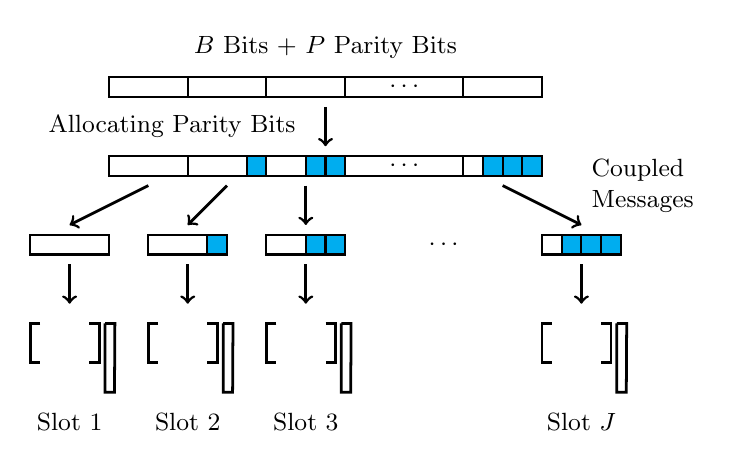
\begin{tikzpicture}
[font=\small, draw=black, line width=0.75pt,
sub0/.style={rectangle, draw, inner sep=0pt, minimum width=10mm,  minimum height=2.5mm},
sub1/.style={rectangle, draw, inner sep=0pt, minimum width=15mm, minimum height=2.5mm},
sub1s/.style={rectangle, inner sep=0pt, minimum width=15mm, minimum height=2.5mm},
parity/.style={rectangle, draw, fill=cyan, inner sep=0pt, minimum size=2.5mm}]

\node (coupledvector) at (2.25,5.50) {$B$~Bits + $P$~Parity Bits};
\node[sub0] (cs0) at (0.00,5) {};
\node[sub0] (cs2) at (1.00,5) {};
\node[sub0] (cs3) at (2.00,5) {};
\node[sub1] (csx) at (3.25,5) {$\cdots$};
\node[sub0] (csz) at (4.50,5) {};

\draw[->, line width=1pt]  (2.25,4.75) -- (2.25,4.25);
\node[anchor=east] (coding) at (2.00,4.50) {Allocating Parity Bits};

\node[sub0] (subcs0) at (0.00,4) {};
\node[sub0] (subcs2) at (1.00,4) {};
\node[parity] (parity0) at (1.375,4) {};
\node[sub0] (subcs3) at (2.00,4) {};
\node[parity] (parity1) at (2.125,4) {};
\node[parity] (parity2) at (2.375,4) {};
\node[sub1] (subcsx) at (3.25,4) {$\cdots$};
\node[sub0] (subcsz) at (4.50,4) {};
\node[parity] (parity3) at (4.375,4) {};
\node[parity] (parity4) at (4.625,4) {};
\node[parity] (parity5) at (4.875,4) {};

\node[sub0] (subcs0) at (-1.00,3) {};
\node[sub0] (subcs2) at (0.50,3) {};
\node[parity] (parity0) at (0.875,3) {};
\node[sub0] (subcs3) at (2.00,3) {};
\node[parity] (parity1) at (2.125,3) {};
\node[parity] (parity2) at (2.375,3) {};
\node[sub1s] (subcsx) at (3.75,3) {$\cdots$};
\node[sub0] (subcsz) at (5.50,3) {};
\node[parity] (parity3) at (5.375,3) {};
\node[parity] (parity4) at (5.625,3) {};
\node[parity] (parity5) at (5.875,3) {};

\draw[->, line width=1pt]  (0.00,3.75) -- (-1.00,3.25);
\draw[->, line width=1pt]  (1.00,3.75) -- (0.50,3.25);
\draw[->, line width=1pt]  (2.00,3.75) -- (2.00,3.25);
\draw[->, line width=1pt]  (4.50,3.75) -- (5.50,3.25);
\node[anchor=west,align=left] (coupledvector) at (5.50,3.75) {Coupled\\Messages};

\foreach \v in {-1.00,0.50,2.00,5.50} {
  \draw[->, line width=1pt]  (\v,2.75) -- (\v,2.25);

  \draw[line width=1pt] (\v-0.375,2) -- (\v-0.5,2) -- (\v-0.5,1.5) -- (\v-0.375,1.5);
  \draw[line width=1pt] (\v+0.25,2) -- (\v+0.375,2) -- (\v+0.375,1.5) -- (\v+0.25,1.5);
  \draw[line width=1pt] (\v+0.45,2) -- (\v+0.45,1.125) -- (\v+0.57,1.125) -- (\v+0.575,2) -- (\v+0.45,2);
}

\node (cs) at (-1.00,0.75) {Slot~1};
\node (cs) at (0.50,0.75) {Slot~2};
\node (cs) at (2.00,0.75) {Slot~3};
\node (cs) at (5.50,0.75) {Slot~$J$};
\end{tikzpicture}

\end{center}
% % % % %
\begin{itemize}
\item Collection of $L$ CS matrices and 1-sparse vectors
\item Each CS generated signal is sent in specific time slot
\end{itemize}
\myfootnote{\tiny
V. K. Amalladinne, J.-F. Chamberland, and K. R. Narayanan. \emph{A coded compressed sensing scheme for unsourced multiple access}. IEEE Transactions on Information Theory, 2020.}
\end{frame}

% % % % % % % % % % % % % % % % % % % %

\begin{frame}
\frametitle{Coded Compressive Sensing -- Multiple Access}
% % % % %
\begin{center}
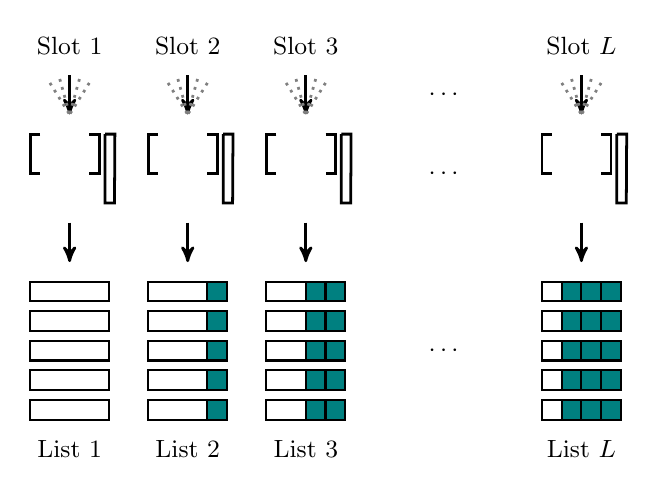
\begin{tikzpicture}
[font=\small, draw=black, line width=0.75pt, >=stealth',
sub0/.style={rectangle, draw, inner sep=0pt, minimum width=10mm, minimum height=2.5mm},
parity/.style={rectangle, draw, fill=teal, inner sep=0pt, minimum size=2.5mm}]

\node (cs1) at (-1.00,6.125) {Slot~1};
\node (cs2) at (0.50,6.125) {Slot~2};
\node (cs3) at (2.00,6.125) {Slot~3};
\node (cs4) at (5.50,6.125) {Slot~$L$};

\foreach \v in {-1.00,0.50,2.00,5.50} {
  \draw[->, line width=1pt]  (\v,3.875) -- (\v,3.375);
  \draw[->, line width=1pt]  (\v,5.75) -- (\v,5.25);
  \draw[dotted, line width=1pt, draw=gray]  (\v-0.25,5.65) -- (\v,5.25);
  \draw[dotted, line width=1pt, draw=gray]  (\v-0.125,5.7) -- (\v,5.25);
  \draw[dotted, line width=1pt, draw=gray]  (\v+0.125,5.7) -- (\v,5.25);
  \draw[dotted, line width=1pt, draw=gray]  (\v+0.25,5.65) -- (\v,5.25);
}

\node (dots1) at (3.75,5.5) {$\cdots$};

\foreach \v in {-1.00,0.50,2.00,5.50} {
  \draw[line width=1pt] (\v-0.375,5) -- (\v-0.5,5) -- (\v-0.5,4.5) -- (\v-0.375,4.5);
  \draw[line width=1pt] (\v+0.25,5) -- (\v+0.375,5) -- (\v+0.375,4.5) -- (\v+0.25,4.5);
  \draw[line width=1pt] (\v+0.45,5) -- (\v+0.45,4.125) -- (\v+0.57,4.125) -- (\v+0.575,5) -- (\v+0.45,5);
}

\node (dots2) at (3.75,4.5) {$\cdots$};
\node (dots3) at (3.75,2.25) {$\cdots$};

\foreach \c in {3.00, 2.625, 2.25, 1.875, 1.5} {
  \node[sub0] (subcs0\c) at (-1.00,\c) {};
  \node[sub0] (subcs2\c) at (0.50,\c) {};
  \node[parity] (parity0\c) at (0.875,\c) {};
  \node[sub0] (subcs3\c) at (2.00,\c) {};
  \node[parity] (parity1\c) at (2.125,\c) {};
  \node[parity] (parity2\c) at (2.375,\c) {};
  \node[sub0] (subcsz\c) at (5.50,\c) {};
  \node[parity] (parity3\c) at (5.375,\c) {};
  \node[parity] (parity4\c) at (5.625,\c) {};
  \node[parity] (parity5\c) at (5.875,\c) {};
}

\node (list1) at (-1.00,1) {List~1};
\node (list2) at (0.50,1) {List~2};
\node (list3) at (2.00,1) {List~3};
\node (list4) at (5.50,1) {List~$L$};
\end{tikzpicture}

\end{center}
% % % % %
\begin{itemize}
\item $L$ instances of CS problem, each solved with non-negative LS
\item Produces $L$ lists of $K$ decoded sub-packets (with parity)
\item Must piece sub-packets together using tree decoder
\end{itemize}
\end{frame}

% % % % % % % % % % % % % % % % % % % %

\begin{frame}
\frametitle{Coded Compressive Sensing -- Stitching Process}
% % % % %
\begin{center}
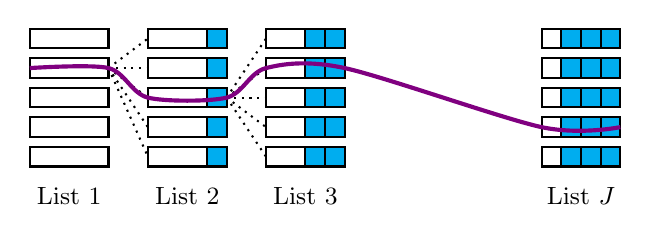
\begin{tikzpicture}
[font=\small, draw=black, line width=0.75pt,
sub0/.style={rectangle, draw, inner sep=0pt, minimum width=10mm, minimum height=2.5mm},
parity/.style={rectangle, draw, fill=cyan, inner sep=0pt, minimum size=2.5mm}]

\foreach \c in {3.00, 2.625, 2.25, 1.875, 1.5} {
  \node[sub0] (subcs1\c) at (-1.00,\c) {};
  \node[sub0] (subcs2\c) at (0.50,\c) {};
  \node[parity] (parity0\c) at (0.875,\c) {};
  \node[sub0] (subcs3\c) at (2.00,\c) {};
  \node[parity] (parity1\c) at (2.125,\c) {};
  \node[parity] (parity2\c) at (2.375,\c) {};
  \node[sub0] (subcsz\c) at (5.50,\c) {};
  \node[parity] (parity3\c) at (5.375,\c) {};
  \node[parity] (parity4\c) at (5.625,\c) {};
  \node[parity] (parity5\c) at (5.875,\c) {};
}

\draw[dotted] (-0.50,2.625) -- (0.00,3.00) {};
\draw[dotted] (-0.50,2.625) -- (0.00,2.625) {};
\draw[dotted] (-0.50,2.625) -- (0.00,2.25) {};
\draw[dotted] (-0.50,2.625) -- (0.00,1.875) {};
\draw[dotted] (-0.50,2.625) -- (0.00,1.50) {};

\draw[dotted] (1.00,2.25) -- (1.50,3.00) {};
\draw[dotted] (1.00,2.25) -- (1.50,2.625) {};
\draw[dotted] (1.00,2.25) -- (1.50,2.25) {};
\draw[dotted] (1.00,2.25) -- (1.50,1.875) {};
\draw[dotted] (1.00,2.25) -- (1.50,1.50) {};

\node (list1) at (-1.00,1) {List~1};
\node (list2) at (0.50,1) {List~2};
\node (list3) at (2.00,1) {List~3};
\node (list4) at (5.50,1) {List~$J$};

\draw [line width=1.5pt,color=violet] plot[smooth, tension=.5] coordinates {
(-1.50,2.625) (-0.50,2.625)
(0.00,2.25) (1.00,2.25)
(1.50,2.625) (2.50,2.625)
(5.00, 1.875) (6.00, 1.875)};
\end{tikzpicture}

\end{center}
% % % % %
\begin{columns}
\column{.45\textwidth}
\begin{block}{Tree decoding principles}
  \begin{itemize}
  \item Every parity is linear combination of bits in preceding blocks
  \item Late parity bits offer better performance
  \item Early parity bits decrease decoding complexity
  \item Correct fragment is on list
  \end{itemize}
\end{block}
\column{.45\textwidth}
  \centerline{\scalebox{0.5}{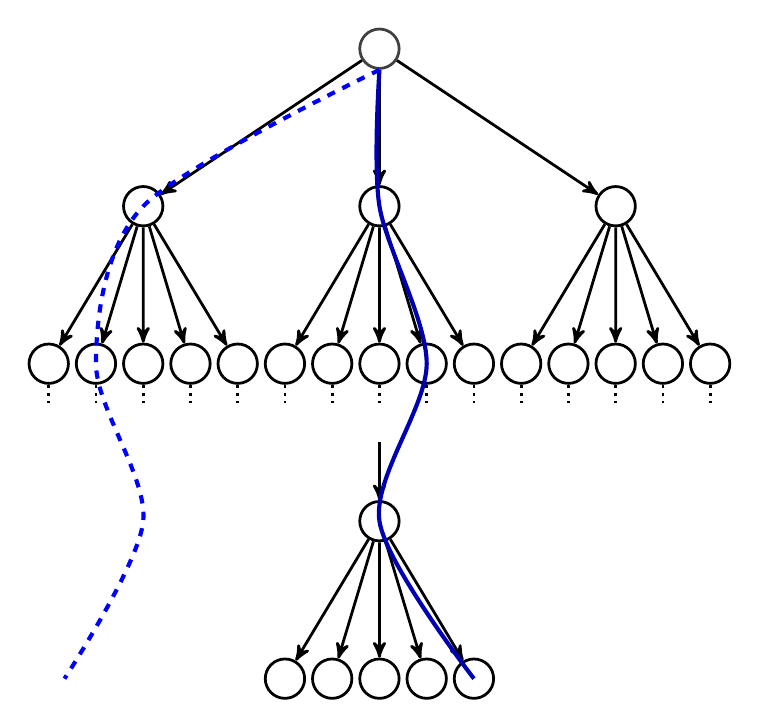
\begin{tikzpicture}
  [
  line width=1pt, draw=black, >=stealth',
  checknode/.style={circle, inner sep=0pt, minimum size=5mm, draw=black}
  ]

  \node[checknode, draw=darkgray] (b1) at (0,4) {};

  \foreach \x in {1,2,3} {
    \node[checknode] (c1\x) at (-6+3*\x,2) {}
      edge[<-] (b1);
  }

  \foreach \y in {1,2,3,4,5} {
    \node[checknode] (b1\y) at (-4.8+0.6*\y,0) {}
      edge[<-] (c11)
      edge[-,dotted] (-4.8+0.6*\y,-0.5);
    \node[checknode] (b2\y) at (-1.8+0.6*\y,0) {}
      edge[<-] (c12)
      edge[-,dotted] (-1.8+0.6*\y,-0.5);
    \node[checknode] (b3\y) at (1.2+0.6*\y,0) {}
      edge[<-] (c13)
      edge[-,dotted] (1.2+0.6*\y,-0.5);
  }
  
  \node[checknode] (c22) at (0,-2) {}
    edge[<-] (0,-1);

  \foreach \y in {1,2,3,4,5} {
    \node[checknode] (b4\y) at (-1.8+0.6*\y,-4) {}
      edge[<-] (c22);
  }

\draw [line width=1.5pt,color=blue!70!black] plot[smooth, tension=.5] coordinates {(b1.south) (c12) (b24) (c22) (b45)};
\draw [line width=1.5pt,dashed, color=blue] plot[smooth, tension=.5] coordinates {(b1.south) (c11) (b12) (-3,-2) (-4,-4)};
\end{tikzpicture}
}}
\end{columns}
\end{frame}

% % % % % % % % % % % % % % % % % % % %

\begin{frame}
\frametitle{Coded Compressive Sensing -- Understanding Parity Bits}
% % % % %
\begin{center}
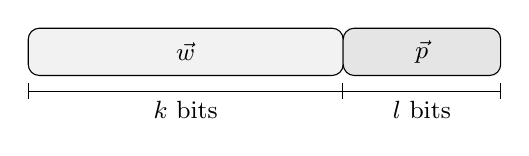
\begin{tikzpicture}[
  font=\small, >=stealth',
  infobits/.style={rectangle, minimum height=6mm, minimum width=40mm, draw=black, fill=gray!10, rounded corners},
  paritybits/.style={rectangle, minimum height=6mm, minimum width=20mm, draw=black, fill=gray!20, rounded corners}
]

\node[infobits] (vb) at (2,0) {$\vec{w}$};
\node[paritybits] (vp) at (5,0) {$\vec{p}$};
\draw[|-|] (0,-0.5) to node[midway,below] {$k$ bits} (4,-0.5);
\draw[-|] (4,-0.5) to node[midway,below] {$l$ bits} (6,-0.5);
\end{tikzpicture}

\end{center}
% % % % %
\begin{itemize}
\item Consider binary information vector $\wv$ of length $k$
\item Systematically encoded using generator matrix $\Gm$, with
$\pv = \wv \Gm$
\item Suppose alternate vector $\wv_{\mathrm{r}}$ is selected at random from $\{ 0, 1 \}^k$
\end{itemize}
% % % % %
\vfill
% % % % %
\begin{block}{Lemma}
Probability that randomly selected information vector $\wv_{\mathrm{r}}$ produces same parity sub-component is given by
\begin{equation*}
\Pr (\pv = \pv_{\mathrm{r}}) = {2^{-\operatorname{rank}(\Gm)}}
\end{equation*}
\end{block}
\structure{Proof:}
%\begin{itemize}
%\item Suppose $\wv_{\mathrm{r}}$ is drawn at random from $\{ 0, 1 \}^k$
%\item Then event $\{ \pv = \pv_{\mathrm{r}} \}$ can equivalently be expressed as
%\begin{equation*}
%\begin{split}
$\{ \pv = \pv_{\mathrm{r}} \}
= \{ \wv \Gm = \wv_{\mathrm{r}} \Gm \}
= \{ \wv + \wv_{\mathrm{r}} \in \operatorname{nullspace}(\Gm) \}$
%\end{split}
%\end{equation*}
%\item Number of vectors in nullspace of $\Gm$ is $2^{\operatorname{nullity}(\Gm)} = 2^{k - \operatorname{rank} (\Gm)}$
%\item Then $\Pr ( \pv = \pv_{\mathrm{r}} )
%= \frac{2^{k - \operatorname{rank} (\Gm)}}{2^k}
%= 2^{- \operatorname{rank} (\Gm)}$
%\end{itemize}
\end{frame}

% % % % % % % % % % % % % % % % % % % %

\begin{frame}
\frametitle{Coded Compressive Sensing -- General Parity Bits}
% % % % %
\begin{center}
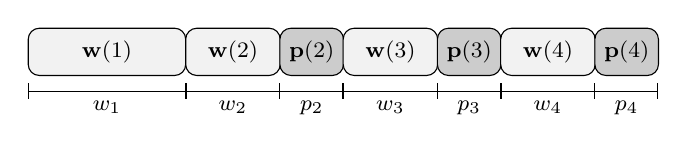
\begin{tikzpicture}[
  font=\footnotesize, >=stealth',
  infobits0/.style={rectangle, minimum height=6mm, minimum width=20mm, draw=black, fill=gray!10, rounded corners},
  infobits/.style={rectangle, minimum height=6mm, minimum width=12mm, draw=black, fill=gray!10, rounded corners},
  paritybits/.style={rectangle, minimum height=6mm, minimum width=8mm, draw=black, fill=gray!40, rounded corners}
]

\node[infobits0] (vb0) at (1,0) {$\wv(1)$};
\node[infobits] (vb1) at (2.6,0) {$\wv(2)$};
\node[paritybits] (vp1) at (3.6,0) {$\pv(2)$};
\node[infobits] (vb2) at (4.6,0) {$\wv(3)$};
\node[paritybits] (vp2) at (5.6,0) {$\pv(3)$};
\node[infobits] (vb3) at (6.6,0) {$\wv(4)$};
\node[paritybits] (vp3) at (7.6,0) {$\pv(4)$};
\draw[|-|] (0,-0.5) to node[midway,below] {$w_1$} (2,-0.5);
\draw[|-|] (2,-0.5) to node[midway,below] {$w_2$} (3.2,-0.5);
\draw[-|] (3.2,-0.5) to node[midway,below] {$p_2$} (4,-0.5);
\draw[|-|] (4,-0.5) to node[midway,below] {$w_3$} (5.2,-0.5);
\draw[-|] (5.2,-0.5) to node[midway,below] {$p_3$} (6,-0.5);
\draw[|-|] (6,-0.5) to node[midway,below] {$w_4$} (7.2,-0.5);
\draw[-|] (7.2,-0.5) to node[midway,below] {$p_4$} (8,-0.5);
\end{tikzpicture}

\end{center}
% % % % %
\begin{itemize}
\item True vector $(\wv_{i_1}(1), \wv_{i_1}(2), \wv_{i_1}(3), \wv_{i_1}(4))$
\item Consider alternate vector with information sub-block $(\wv_{i_1}(1), \wv_{i_2}(2), \wv_{i_3}(3), \wv_{i_4}(4))$ pieced from lists
\item To survive stage~4, candidate vector must fulfill parity equations
\end{itemize}
\begin{align*}
\left( \wv_{i_1}(1) - \wv_{i_2}(1) \right) \begin{bmatrix} \Gm_{1,2} \end{bmatrix} &= \zerov \\
\left( \wv_{i_1}(1) - \wv_{i_3}(1), \wv_{i_2}(2) - \wv_{i_3}(2) \right)
\begin{bmatrix} \Gm_{1,3} \\ \Gm_{2,3} \end{bmatrix}
&= \zerov \\
\left( \wv_{i_1}(1) - \wv_{i_4}(1), \wv_{i_2}(2) - \wv_{i_4}(2), \wv_{i_3}(3) - \wv_{i_4}(3) \right)
\begin{bmatrix} \Gm_{1,4} \\ \Gm_{2,4} \\ \Gm_{3,4} \end{bmatrix}
&= \zerov
\end{align*}
\end{frame}

% % % % % % % % % % % % % % % % % % % %

\begin{frame}
\frametitle{Coded Compressive Sensing -- General Parity Bits}
% % % % %
\begin{center}
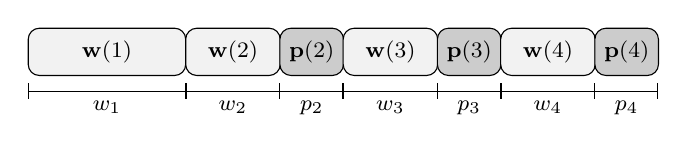
\begin{tikzpicture}[
  font=\footnotesize, >=stealth',
  infobits0/.style={rectangle, minimum height=6mm, minimum width=20mm, draw=black, fill=gray!10, rounded corners},
  infobits/.style={rectangle, minimum height=6mm, minimum width=12mm, draw=black, fill=gray!10, rounded corners},
  paritybits/.style={rectangle, minimum height=6mm, minimum width=8mm, draw=black, fill=gray!40, rounded corners}
]

\node[infobits0] (vb0) at (1,0) {$\wv(1)$};
\node[infobits] (vb1) at (2.6,0) {$\wv(2)$};
\node[paritybits] (vp1) at (3.6,0) {$\pv(2)$};
\node[infobits] (vb2) at (4.6,0) {$\wv(3)$};
\node[paritybits] (vp2) at (5.6,0) {$\pv(3)$};
\node[infobits] (vb3) at (6.6,0) {$\wv(4)$};
\node[paritybits] (vp3) at (7.6,0) {$\pv(4)$};
\draw[|-|] (0,-0.5) to node[midway,below] {$w_1$} (2,-0.5);
\draw[|-|] (2,-0.5) to node[midway,below] {$w_2$} (3.2,-0.5);
\draw[-|] (3.2,-0.5) to node[midway,below] {$p_2$} (4,-0.5);
\draw[|-|] (4,-0.5) to node[midway,below] {$w_3$} (5.2,-0.5);
\draw[-|] (5.2,-0.5) to node[midway,below] {$p_3$} (6,-0.5);
\draw[|-|] (6,-0.5) to node[midway,below] {$w_4$} (7.2,-0.5);
\draw[-|] (7.2,-0.5) to node[midway,below] {$p_4$} (8,-0.5);
\end{tikzpicture}

\end{center}
% % % % %
\begin{itemize}
\item When indices are not repeated in $(\wv_{i_1}(1), \wv_{i_2}(2), \wv_{i_3}(3), \wv_{i_4}(4))$, probability is governed by
\begin{equation*}
\operatorname{rank}
\left(
\begin{bmatrix}
\Gm_{1,2} & \Gm_{1,3} & \Gm_{1,4} \\
\mathbf{0} & \Gm_{2,3} & \Gm_{2,4} \\
\mathbf{0} & \mathbf{0}& \Gm_{3,4}
\end{bmatrix}
\right)
\end{equation*}
\item But, when indices are repeated, sub-blocks may disappear
\begin{equation*}
\operatorname{rank}
\left(
\begin{bmatrix}
\Gm_{1,2} \mathbf{1}_{\{ i_2 \neq i_1 \}} & \Gm_{1,3} \mathbf{1}_{\{ i_3 \neq i_1 \}} & \Gm_{1,4} \mathbf{1}_{\{ i_4 \neq i_1 \}} \\
\mathbf{0} & \Gm_{2,3} \mathbf{1}_{\{ i_3 \neq i_2 \}} & \Gm_{2,4} \mathbf{1}_{\{ i_4 \neq i_2 \}} \\
\mathbf{0} & \mathbf{0}& \Gm_{3,4} \mathbf{1}_{\{ i_4 \neq i_3 \}}
\end{bmatrix}
\right)
\end{equation*}
\end{itemize}
\end{frame}

% % % % % % % % % % % % % % % % % % % %

\begin{frame}
\frametitle{Candidate Paths and Bell Numbers}
% % % % %
\begin{columns}
\column{0.55\textwidth}
  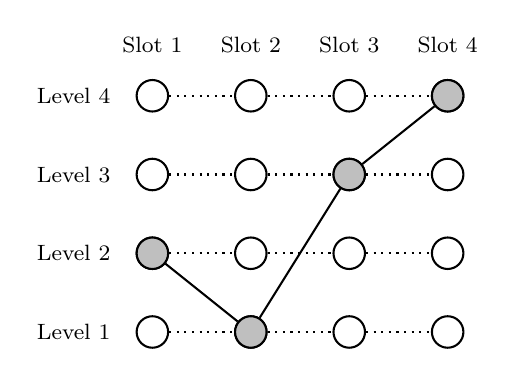
\begin{tikzpicture}
  [
  font=\footnotesize, line width=0.75pt, draw=black,
  subblock/.style={circle, inner sep = 0pt, minimum size = 4mm, draw=black}
  ]

\foreach \x in {1,2,3,4} {
  \foreach \y in {1,2,3,4} {
    \node[subblock] (x{\x}y{\y}) at (1.25*\x - 1.25,\y) {};
  }
  \node (s{\x}) at (1.25*\x - 1.25,4.65) {Slot~\x};
}
\foreach \y in {1,2,3,4} {
  \node (l{\y}) at (-1,\y) {Level~\y};
}

\foreach \y in {1,2,3,4} {
  \draw[dotted](x{1}y{\y}) -- (x{2}y{\y});
  \draw[dotted](x{2}y{\y}) -- (x{3}y{\y});
  \draw[dotted](x{3}y{\y}) -- (x{4}y{\y});
}

\node[subblock,fill=lightgray] (px1y2) at (0,2) {};
\node[subblock,fill=lightgray] (px2y1) at (1.25,1) {}
  edge (px1y2);
\node[subblock,fill=lightgray] (px3y3) at (2.5,3) {}
  edge (px2y1);
\node[subblock,fill=lightgray] (px4y4) at (3.75,4) {}
  edge (px3y3);

\end{tikzpicture}

\column{0.43\textwidth}
  Probability that wrong path is consistent with parities is
  \begin{equation*}
  \Pr (\pv = \pv_{\mathrm{r}}) = {2^{-\operatorname{rank}(\Gm)}}
  \end{equation*}
  where
  \begin{equation*}
  \Gm = \begin{bmatrix}
  \Gm_{1,2} & \Gm_{1,3} & \Gm_{1,4} \\
  \mathbf{0} & \Gm_{2,3} & \Gm_{2,4} \\
  \mathbf{0} & \mathbf{0}& \Gm_{3,4}
  \end{bmatrix}
  \end{equation*}
\end{columns}
% % % % %
\vfill
% % % % %
\begin{center}
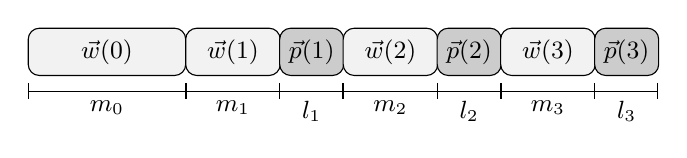
\begin{tikzpicture}[
  font=\small, >=stealth',
  infobits0/.style={rectangle, minimum height=6mm, minimum width=20mm, draw=black, fill=gray!10, rounded corners},
  infobits/.style={rectangle, minimum height=6mm, minimum width=12mm, draw=black, fill=gray!10, rounded corners},
  paritybits/.style={rectangle, minimum height=6mm, minimum width=8mm, draw=black, fill=gray!40, rounded corners}
]

\node[infobits0] (vb0) at (1,0) {$\vec{w}(0)$};
\node[infobits] (vb1) at (2.6,0) {$\vec{w}(1)$};
\node[paritybits] (vp1) at (3.6,0) {$\vec{p}(1)$};
\node[infobits] (vb2) at (4.6,0) {$\vec{w}(2)$};
\node[paritybits] (vp2) at (5.6,0) {$\vec{p}(2)$};
\node[infobits] (vb3) at (6.6,0) {$\vec{w}(3)$};
\node[paritybits] (vp3) at (7.6,0) {$\vec{p}(3)$};
\draw[|-|] (0,-0.5) to node[midway,below] {$m_0$} (2,-0.5);
\draw[|-|] (2,-0.5) to node[midway,below] {$m_1$} (3.2,-0.5);
\draw[-|] (3.2,-0.5) to node[midway,below] {$l_1$} (4,-0.5);
\draw[|-|] (4,-0.5) to node[midway,below] {$m_2$} (5.2,-0.5);
\draw[-|] (5.2,-0.5) to node[midway,below] {$l_2$} (6,-0.5);
\draw[|-|] (6,-0.5) to node[midway,below] {$m_3$} (7.2,-0.5);
\draw[-|] (7.2,-0.5) to node[midway,below] {$l_3$} (8,-0.5);
\end{tikzpicture}
 \\[2mm]
\structure{When Levels Do NOT Repeat}
\end{center}
\end{frame}

% % % % % % % % % % % % % % % % % % % %

\begin{frame}
\frametitle{Candidate Paths and Bell Numbers}
% % % % %
\begin{columns}
\column{0.55\textwidth}
  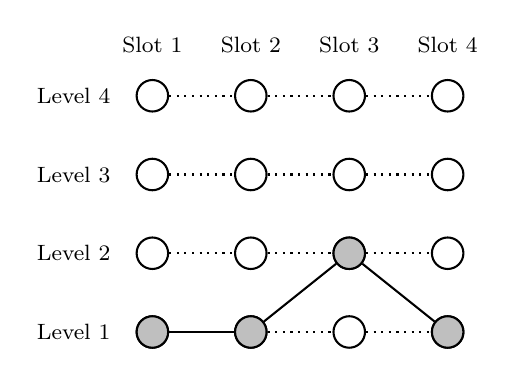
\begin{tikzpicture}
  [
  font=\footnotesize, line width=0.75pt, draw=black,
  subblock/.style={circle, inner sep = 0pt, minimum size = 4mm, draw=black}
  ]

\foreach \x in {1,2,3,4} {
  \foreach \y in {1,2,3,4} {
    \node[subblock] (x{\x}y{\y}) at (1.25*\x - 1.25,\y) {};
  }
  \node (s{\x}) at (1.25*\x - 1.25,4.65) {Slot~\x};
}
\foreach \y in {1,2,3,4} {
  \node (l{\y}) at (-1,\y) {Level~\y};
}

\foreach \y in {1,2,3,4} {
  \draw[dotted](x{1}y{\y}) -- (x{2}y{\y});
  \draw[dotted](x{2}y{\y}) -- (x{3}y{\y});
  \draw[dotted](x{3}y{\y}) -- (x{4}y{\y});
}

\node[subblock,fill=lightgray] (px1y1) at (0,1) {};
\node[subblock,fill=lightgray] (px2y1) at (1.25,1) {}
  edge (px1y1);
\node[subblock,fill=lightgray] (px3y2) at (2.5,2) {}
  edge (px2y1);
\node[subblock,fill=lightgray] (px4y1) at (3.75,1) {}
  edge (px3y2);

\end{tikzpicture}

\column{0.43\textwidth}
  Probability that wrong path is consistent with parities is
  \begin{equation*}
  \Pr (\pv = \pv_{\mathrm{r}}) = {2^{-\operatorname{rank}(\Gm)}}
  \end{equation*}
  where
  \begin{equation*}
  \Gm = \begin{bmatrix}
  \mathbf{0} & \Gm_{1,3} & \mathbf{0} \\
  \mathbf{0} & \Gm_{2,3} & \mathbf{0} \\
  \mathbf{0} & \mathbf{0}& \Gm_{3,4}
  \end{bmatrix}
  \end{equation*}
\end{columns}
% % % % %
\vfill
% % % % %
\begin{center}
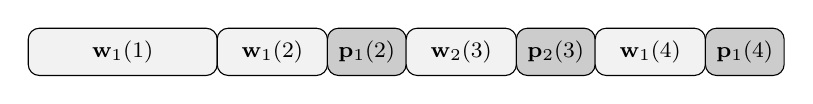
\begin{tikzpicture}[
  font=\footnotesize, >=stealth',
  infobits0/.style={rectangle, minimum height=6mm, minimum width=24mm, draw=black, fill=gray!10, rounded corners},
  infobits/.style={rectangle, minimum height=6mm, minimum width=14mm, draw=black, fill=gray!10, rounded corners},
  paritybits/.style={rectangle, minimum height=6mm, minimum width=10mm, draw=black, fill=gray!40, rounded corners}
]

\node[infobits0] (vb0) at (1.2,0) {$\wv_1(1)$};
\node[infobits] (vb1) at (3.1,0) {$\wv_1(2)$};
\node[paritybits] (vp1) at (4.3,0) {$\pv_1(2)$};
\node[infobits] (vb2) at (5.5,0) {$\wv_2(3)$};
\node[paritybits] (vp2) at (6.7,0) {$\pv_2(3)$};
\node[infobits] (vb3) at (7.9,0) {$\wv_1(4)$};
\node[paritybits] (vp3) at (9.1,0) {$\pv_1(4)$};
\end{tikzpicture}
 \\[2mm]
\structure{When Levels Repeat}
\end{center}
\end{frame}

% % % % % % % % % % % % % % % % % % % %

\begin{frame}{Bell Numbers and $j$-patterns}
\begin{columns}
% % % % %
\column{0.42\textwidth}
  \begin{block}{Integer Sequences}
  \begin{itemize}
  \item $K^L$ paths
  \item Reduce complexity through equivalence
  \item Online Encyclopedia of Integer Sequences (OEIS) A000110
  \item Bell numbers grow rapidly
  \item Hard to compute expected number of surviving paths
  \end{itemize}
  \end{block}
\column{0.55\textwidth}
  \scalebox{0.75}{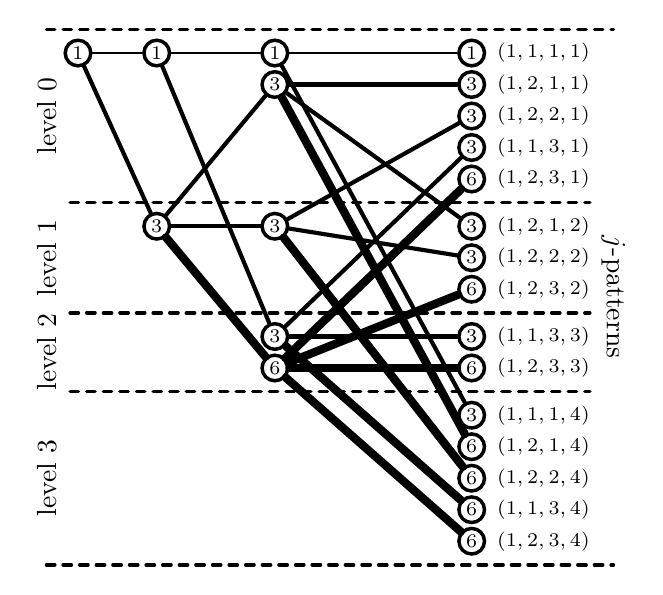
\begin{tikzpicture}[
  font=\scriptsize, >=stealth', line width=1.25pt, line cap=round,
  node/.style={circle, minimum size=3.25mm, inner sep=0pt, draw=black}
]

\node[node] (s1) at (0,3.1) {1};
  \node[node] (s1-1) at (1,3.1) {1};
    \node[node] (s1-1-1) at (2.5,3.1) {1};
      \node[node,label=right:{$(1,1,1,1)$}] (s1-1-1-1) at (5,3.1) {1};
      \node[node,label=right:{$(1,1,1,4)$}] (s1-1-1-4) at (5,-1.5) {3};
    \node[node] (s1-1-3) at (2.5,-0.5) {3};
      \node[node,label=right:{$(1,1,3,1)$}] (s1-1-3-1) at (5,1.9) {3};
      \node[node,label=right:{$(1,1,3,3)$}] (s1-1-3-3) at (5,-0.5) {3};
      \node[node,label=right:{$(1,1,3,4)$}] (s1-1-3-4) at (5,-2.7) {6};
  \node[node] (s1-2) at (1,0.9) {3};
    \node[node] (s1-2-1) at (2.5,2.7) {3};
      \node[node,label=right:{$(1,2,1,1)$}] (s1-2-1-1) at (5,2.7) {3};
      \node[node,label=right:{$(1,2,1,2)$}] (s1-2-1-2) at (5,0.9) {3};
      \node[node,label=right:{$(1,2,1,4)$}] (s1-2-1-4) at (5,-1.9) {6};
    \node[node] (s1-2-2) at (2.5,0.9) {3};
      \node[node,label=right:{$(1,2,2,1)$}] (s1-2-2-1) at (5,2.3) {3};
      \node[node,label=right:{$(1,2,2,2)$}] (s1-2-2-2) at (5,0.5) {3};
      \node[node,label=right:{$(1,2,2,4)$}] (s1-2-2-4) at (5,-2.3) {6};
    \node[node] (s1-2-3) at (2.5,-0.9) {6};
      \node[node,label=right:{$(1,2,3,1)$}] (s1-2-3-1) at (5,1.5) {6};
      \node[node,label=right:{$(1,2,3,2)$}] (s1-2-3-2) at (5,0.1) {6};
      \node[node,label=right:{$(1,2,3,3)$}] (s1-2-3-3) at (5,-0.9) {6};
      \node[node,label=right:{$(1,2,3,4)$}] (s1-2-3-4) at (5,-3.1) {6};

\draw[line width=0.5pt] (s1) -- (s1-1);
  \draw[line width=0.5pt] (s1-1) -- (s1-1-1);
    \draw[line width=0.5pt] (s1-1-1) -- (s1-1-1-1);
    \draw[line width=1.5pt] (s1-1-1) -- (s1-1-1-4);
  \draw[line width=1.5pt] (s1-1) -- (s1-1-3);
    \draw[line width=1.5pt] (s1-1-3) -- (s1-1-3-1);
    \draw[line width=1.5pt] (s1-1-3) -- (s1-1-3-3);
    \draw[line width=3.0pt] (s1-1-3) -- (s1-1-3-4);
\draw[line width=1.5pt] (s1) -- (s1-2);
  \draw[line width=1.5pt] (s1-2) -- (s1-2-1);
    \draw[line width=1.5pt] (s1-2-1) -- (s1-2-1-1);
    \draw[line width=1.5pt] (s1-2-1) -- (s1-2-1-2);
    \draw[line width=3.0pt] (s1-2-1) -- (s1-2-1-4);
  \draw[line width=1.5pt] (s1-2) -- (s1-2-2);
    \draw[line width=1.5pt] (s1-2-2) -- (s1-2-2-1);
    \draw[line width=1.5pt] (s1-2-2) -- (s1-2-2-2);
    \draw[line width=3.0pt] (s1-2-2) -- (s1-2-2-4);
  \draw[line width=3.0pt] (s1-2) -- (s1-2-3);
    \draw[line width=3.0pt] (s1-2-3) -- (s1-2-3-1);
    \draw[line width=3.0pt] (s1-2-3) -- (s1-2-3-2);
    \draw[line width=3.0pt] (s1-2-3) -- (s1-2-3-3);
    \draw[line width=3.0pt] (s1-2-3) -- (s1-2-3-4);

\draw[dashed] (-0.4,3.4) -- (6.8,3.4);
\draw[dashed] (-0.1,1.2) -- (6.5,1.2);
\draw[dashed] (-0.1,-0.2) -- (6.5,-0.2);
\draw[dashed] (-0.1,-1.2) -- (6.5,-1.2);
\draw[dashed] (-0.4,-3.4) -- (6.8,-3.4);

\node[rotate=90] at (-0.4,2.3) {\normalsize level~$0$};
\node[rotate=90] at (-0.4,0.5) {\normalsize level~$1$};
\node[rotate=90] at (-0.4,-0.7) {\normalsize level~$2$};
\node[rotate=90] at (-0.4,-2.3) {\normalsize level~$3$};

\node[rotate=-90] at (6.8,0) {\normalsize $j$-patterns};
\end{tikzpicture}
}
\end{columns}
% % % % %
\vfill
% % % % %
\begin{center}
\begin{tikzpicture}
\shade[draw=none,
left color={rgb:red,1;green,2;blue,3},
right color=frametitle.fg,
shading angle=60,
rounded corners,
blur shadow={shadow blur steps=5}] (-2.75,-0.625) rectangle (2.75,0.625);
\shade[fill=white, fill opacity=0.1] (-2.75,-0.625) rectangle (2.75,0.625);
\node at (0,0) {\textcolor{white}{\Large \textbf{
Need Approximation}}};
\end{tikzpicture}
\end{center}
\end{frame}

% % % % % % % % % % % % % % % % % % % %

\begin{frame}
\frametitle{Allocating Parity Bits (approximation)}
% % % % %
\begin{itemize}
\item $p_{\ell}$: \# parity bits in sub-block $\ell \in 2, \ldots, L$,
\item $P_{\ell}$: \# erroneous paths that survive stage $\ell \in 2, \ldots, L$,
\item Complexity $C_{\mathrm{tree}}$: \# nodes on which parity check constraints verified
\end{itemize}
% % % % %
\vfill
% % % % %
\begin{block}{Expressions for $\mathbb{E}[P_{\ell}]$ and $C_{\mathrm{tree}}$}
\begin{itemize}
\item $P_{\ell} \lvert P_{\ell-1} \sim B((P_{\ell-1}+1)K-1,\rho_{\ell})$, $\rho_{\ell}=2^{-p_{\ell}}$, $q_{\ell}=1-\rho_{\ell}$
\begin{align*}
\mathbb{E}[P_{\ell}] &= \mathbb{E}[ \mathbb{E}[P_{\ell} \lvert P_{\ell-1}]] \\
&= \mathbb{E}[((P_{\ell-1}+1)K-1)\rho_{\ell}] \\
&= \rho_{\ell} K\mathbb{E}[P_{\ell-1}] + \rho_{\ell}(K-1) \\
&= \sum_{r=1}^{\ell} K^{\ell-r}(K-1) \prod_{j=r}^{\ell}\rho_j
\end{align*}
\item $C_{\mathrm{tree}} = K + \sum_{\ell=2}^{L-1}\left[(P_{\ell} + 1)K\right]$
\item $\mathbb{E}[C_{\mathrm{tree}}]$ can be computed using the expression for $\mathbb{E}[P_{\ell}]$
\end{itemize}
\end{block}
\end{frame}

% % % % % % % % % % % % % % % % % % % %

\begin{frame}
\frametitle{Optimization of Parity Lengths}
% % % % %
\begin{itemize}
\item $p_{\ell}$: \# parity bits in sub-block $\ell \in 2, \ldots, L$,
\item $P_{\ell}$: \# erroneous paths that survive stage $\ell \in 2, \ldots, L$,
\end{itemize}
% % % % %
\vfill
% % % % %
\begin{block}{Relaxed geometric programming optimization}
\blockmathspace
\begin{equation*}
\begin{aligned}
& \underset{(p_2, \dots, p_{L})}{\text{minimize}}
& &\mathbb{E}[C_{\mathrm{tree}}] \\
& \text{subject to}
& & \Pr(P_{L} \ge 1) \le \varepsilon_{\mathrm{tree}}
& \text{\textcolor{frametitle.fg}{Erroneous paths}} \\
&&& \sum_{\ell=2}^{L} p_{\ell} = M-B & \text{\textcolor{frametitle.fg}{Total \# parity bits}} \\
&&& p_{\ell} \in \{ 0, \ldots, N/L \} \quad \forall~\ell \in 2, \ldots, L
& \text{\textcolor{frametitle.fg}{Integer constraints}}
\end{aligned}
\end{equation*}
\end{block}
% % % % %
\vfill
% % % % %
\begin{itemize}
\item Solved using standard convex solver, e.g., CVX
\end{itemize}
\end{frame}

% % % % % % % % % % % % % % % % % % % %

\begin{frame}
\frametitle{Choice of Parity Lengths}
% % % % %
\begin{itemize}
\item $K=200$, $L=11$, $N/L=15$
\end{itemize}
% % % % %
\vfill
% % % % %
\begin{center}
\begin{tabular}{||l|l|l||}
\hline
 $\varepsilon_{\mathrm{tree}}$ & $\mathbb{E}[C_{\mathrm{tree}}]$ & Parity Lengths $p_2, \ldots, p_L$ \\[0.5ex]
\hline \hline
$0.006$ & Infeasible & Infeasible \tabularnewline
\hline
$0.0061930$ & $3.2357\times10^{11}$ & $ 0 ,0, 0, 0, 15, 15, 15, 15, 15, 15$ \tabularnewline
\hline
$0.0061931$ & $3357300$ & $ 0, 3, 8, 8, 8, 8, 10, 15, 15, 15$ \tabularnewline
\hline
$0.0061932$ & $1737000$ & $ 0, 4, 8, 8, 8, 8, 9, 15, 15, 15$ \tabularnewline
\hline
$0.0061933$ & $926990$ & $ 0, 5, 8, 8, 8, 8, 8, 15, 15, 15$ \tabularnewline
\hline
$0.0061935$ & $467060$ & $ 1, 8, 8, 8, 8, 8, 8, 11, 15, 15$ \tabularnewline
\hline
$0.0062$ & $79634$ & $ 1, 8, 8, 8, 8, 8, 8, 11, 15, 15$ \tabularnewline
\hline
$0.007$ & $7357.8$ & $ 6, 8, 8, 8, 8, 8, 8, 8, 13, 15$ \tabularnewline
\hline
$0.008$ & $6152.7$ & $ 7, 8, 8, 8, 8, 8, 8, 8, 12, 15$ \tabularnewline
\hline
$0.02$ & $5022.9$ & $ 6, 8, 8, 9, 9, 9, 9, 9, 9, 14$ \tabularnewline
\hline
$0.04$ & $4158$ & $ 7, 8, 8, 9, 9, 9, 9, 9, 9, 13$ \tabularnewline
\hline
$0.6378$ & $3066.3$ & $ 9, 9, 9, 9, 9, 9, 9, 9, 9, 9$ \tabularnewline
\hline
\end{tabular}
\end{center}
\end{frame}

% % % % % % % % % % % % % % % % % % % %

\begin{frame}
\frametitle{Choice of Parity Lengths}
% % % % %
\begin{itemize}
\item $K=200$, $L=11$, $N/L=15$
\end{itemize}
\vfill
\begin{columns}
\column{0.45\textwidth}
\centerline{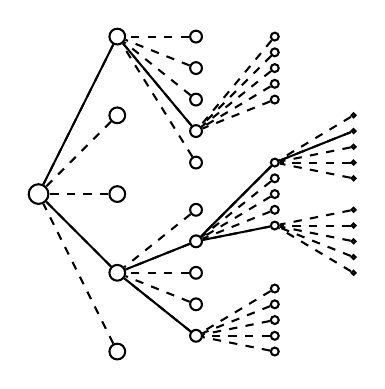
\begin{tikzpicture}
[font=\footnotesize, draw=black, line width=0.75pt,
fragment/.style={circle, draw, inner sep=0pt}]

\node[fragment,minimum size=2.5mm] (x0y0) at (0, 2) {};
\foreach \y in {0, ..., 4} {
    \node[fragment,minimum size=2mm] (x1y\y) at (1, \y) {}
        edge[dashed] (x0y0);
}
\draw (x0y0) -- (x1y4);
\draw (x0y0) -- (x1y1);

\foreach \y/\p in {51/2.4, 52/2.8, 53/3.2,  54/3.6, 55/4.0} {
    \node[fragment,minimum size=1.5mm] (x2y\y) at (2, \p) {}
        edge[dashed] (x1y4);
}
\draw (x1y4) -- (x2y52);

\foreach \y/\p in {21/0.2, 22/0.6, 23/1.0,  24/1.4, 25/1.8} {
    \node[fragment,minimum size=1.5mm] (x2y\y) at (2, \p) {}
        edge[dashed] (x1y1);
}
\draw (x1y1) -- (x2y24);
\draw (x1y1) -- (x2y21);

\foreach \y/\p in {421/3.2, 422/3.4, 423/3.6,  424/3.8, 425/4.0} {
    \node[fragment,minimum size=1mm] (x3y\y) at (3, \p) {}
        edge[dashed] (x2y52);
}

\foreach \y/\p in {241/1.6, 242/1.8, 243/2.0,  244/2.2, 245/2.4} {
    \node[fragment,minimum size=1mm] (x3y\y) at (3, \p) {}
        edge[dashed] (x2y24);
}
\draw (x2y24) -- (x3y241);
\draw (x2y24) -- (x3y245);

\foreach \y/\p in {211/0.0, 212/0.2, 213/0.4,  214/0.6, 215/0.8} {
    \node[fragment,minimum size=1mm] (x3y\y) at (3, \p) {}
        edge[dashed] (x2y21);
}

\foreach \y/\p in {2451/2.2, 2452/2.4, 2453/2.6,  2454/2.8, 2455/3.0} {
    \node[fragment,minimum size=0.5mm] (x4y\y) at (4, \p) {}
        edge[dashed] (x3y245);
}
\draw (x3y245) -- (x4y2454);

\foreach \y/\p in {2411/1.0, 2412/1.2, 2413/1.4,  2414/1.6, 2415/1.8} {
    \node[fragment,minimum size=0.5mm] (x4y\y) at (4, \p) {}
        edge[dashed] (x3y241);
}

\end{tikzpicture}}
\column{0.5\textwidth}
\begin{tabular}{|l||}
\hline
Parity Lengths $p_2, \ldots, p_L$ \\[0.5ex]
\hline \hline
$ 0 ,0, 0, 0, 15, 15, 15, 15, 15, 15$ \tabularnewline
\hline
$ 0, 3, 8, 8, 8, 8, 10, 15, 15, 15$ \tabularnewline
\hline
$ 0, 4, 8, 8, 8, 8, 9, 15, 15, 15$ \tabularnewline
\hline
$ 0, 5, 8, 8, 8, 8, 8, 15, 15, 15$ \tabularnewline
\hline
$ 1, 8, 8, 8, 8, 8, 8, 11, 15, 15$ \tabularnewline
\hline
$ 1, 8, 8, 8, 8, 8, 8, 11, 15, 15$ \tabularnewline
\hline
$ 6, 8, 8, 8, 8, 8, 8, 8, 13, 15$ \tabularnewline
\hline
$ 7, 8, 8, 8, 8, 8, 8, 8, 12, 15$ \tabularnewline
\hline
$ 6, 8, 8, 9, 9, 9, 9, 9, 9, 14$ \tabularnewline
\hline
$ 7, 8, 8, 9, 9, 9, 9, 9, 9, 13$ \tabularnewline
\hline
$ 9, 9, 9, 9, 9, 9, 9, 9, 9, 9$ \tabularnewline
\hline
\end{tabular}
\end{columns}
\end{frame}

% % % % % % % % % % % % % % % % % % % %

\begin{frame}
\frametitle{Performance of CCS and Previous Schemes}
% % % % %
\begin{center}
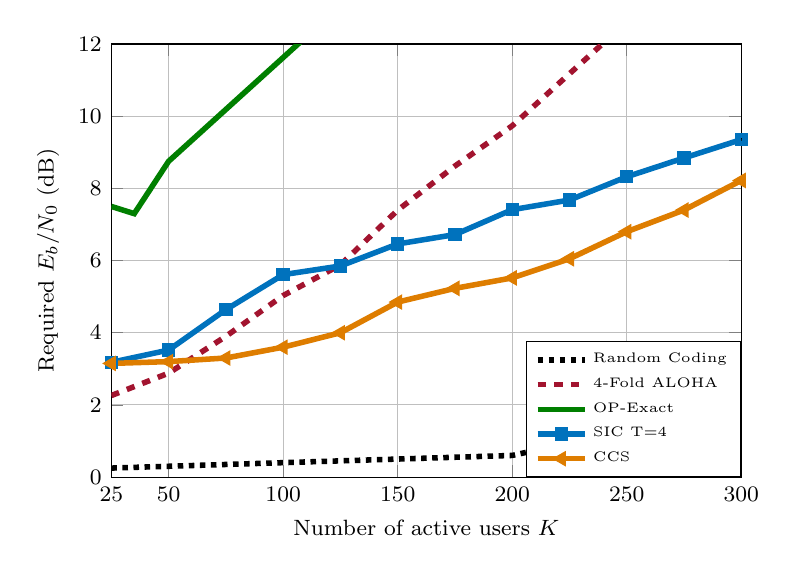
\begin{tikzpicture}
\definecolor{mycolor1}{rgb}{0.63529,0.07843,0.18431}%
\definecolor{mycolor2}{rgb}{0.00000,0.44706,0.74118}%
\definecolor{mycolor3}{rgb}{0.00000,0.49804,0.00000}%
\definecolor{mycolor4}{rgb}{0.87059,0.49020,0.00000}%
\definecolor{mycolor5}{rgb}{0.00000,0.44700,0.74100}%
\definecolor{mycolor6}{rgb}{0.74902,0.00000,0.74902}%

\begin{axis}[%
font=\footnotesize,
width=8cm,
height=5.5cm,
scale only axis,
xmin=25,
xmax=300,
xtick = {25,50,100,...,300},
xlabel={Number of active users $K$},
xmajorgrids,
ymin=0,
ymax=12,
ytick = {0,2,...,12},
ylabel={Required $E_b/N_0$ (dB)},
ylabel near ticks,
ymajorgrids,
legend style={font=\tiny, at={(1,0)},anchor=south east, draw=black,fill=white,legend cell align=left}
]

\addplot [color=black,dotted,line width=2.0pt]
  table[row sep=crcr]{
 25	0.25\\
50	0.3\\
75	0.35\\
100	0.4\\
125	0.45\\
150	0.5\\
175	0.55\\
200	0.6\\
225	0.95\\
250	1.25\\
275	1.55\\
300	1.8\\
};
\addlegendentry{Random Coding};

\addplot [color=mycolor1,dashed,line width=2.0pt]
  table[row sep=crcr]{25	2.26\\
50	2.88\\
75	3.9\\
100	5.03\\
125	5.8798\\
150	7.3954\\
175	8.6199\\
200	9.7328\\
225	11.1761\\
250	12.6127\\
275	13.3907\\
300	14.9116\\
};
\addlegendentry{4-Fold ALOHA};

\addplot [color=mycolor3,solid,line width=2.0pt]
  table[row sep=crcr]{25	7.5\\
35	7.3\\
50	8.75\\
%100	11.7\\
150	14.5\\
200	18\\
250	21\\
300	23\\
};
\addlegendentry{OP-Exact};

\addplot [color=mycolor2,solid,line width=2.0pt,mark size=1.4pt,mark=square,mark options={solid}]
  table[row sep=crcr]{25	3.18\\
50	3.52\\
75	4.64\\
100	5.61\\
125	5.85\\
150	6.46\\
175	6.72\\
200	7.41\\
225	7.6772\\
250	8.3217\\
275	8.8428\\
300	9.352\\
};
\addlegendentry{SIC T=4};

\addplot [color=mycolor4,solid,line width=2.0pt,mark size=1.3pt,mark=triangle,mark options={solid,rotate=90}]
  table[row sep=crcr]{
  25  3.15\\
50	3.2\\
75	3.3\\
100	3.6\\
125	4\\
150	4.85\\
175	5.23\\
200	5.52\\
225	6.05\\
250	6.8\\
275	7.4\\
300	8.22\\
};
\addlegendentry{CCS};

%\addplot [color=black,solid,line width=2.0pt]
%  table[row sep=crcr]{
%25	3\\
%50	3.5\\
%75  3.5\\
%100	4\\
%125	4\\
%150 4.5\\
%175 5\\
%200	5\\
%225 5.5
%250	5.8\\
%275 5.8\\
%300	6\\
%};
%\addlegendentry{AMP+Tree Code};

%\addplot [color=mycolor3,solid,line width=2.0pt,mark size=1.4pt,mark=square,mark options={solid}]
%  table[row sep=crcr]{
%  25  2\\
%50	2.1\\
%75	2.2\\
%100	2.41\\
%125	2.57\\
%150	2.81\\
%175	3\\
%200 3.4\\
%225 3.88\\
%250 4.36\\
%275 4.87\\
%300 5.35\\
%};
%\addlegendentry{Sparse IDMA};
%\node[] at (axis cs: 300,5.15) {\scriptsize \textcolor{red}{O}};
%\node[] at (axis cs: 275,4.69) {\scriptsize \textcolor{red}{O}};
%\node[] at (axis cs: 225,3.7) {\scriptsize \textcolor{red}{O}};

%\addplot [color=violet,solid,line width=2.0pt]
%  table[row sep=crcr]{
%10 0.3801\\
%20 0.5939\\
%30 0.8524\\
%40 0.9949\\
%50 1.1553\\
%60 1.3246\\
%70 1.5474\\
%80 1.7167\\
%90 1.8682\\
%100 2.0554\\
%110 2.2247\\
%120 2.3762\\
%130 2.5811\\
%140 2.7950\\
%150 2.9999\\
%160 3.1425\\
%170 3.3475\\
%180 3.5168\\
%190 3.7128\\
%200 3.8911\\
%210 4.0425\\
%220 4.2742\\
%230 4.5505\\
%240 4.7554\\
%250 4.9158\\
%260 5.0762\\
%270 5.2010\\
%280 5.3168\\
%290 5.4059\\
%300 5.4951\\
%310 5.5663\\
%320 5.6376\\
%330 5.6911\\
%340 5.7357\\
%350 5.7624\\
%360 5.7802\\
%370 5.8069\\
%380 5.8248\\
%390 5.8515\\
%400 5.9050\\
%410 6.0119\\
%420 6.1634\\
%430 6.6000\\
%};
%\addlegendentry{Polar Codes};

\end{axis}


\end{tikzpicture}%


\end{center}
\end{frame}

% % % % % % % % % % % % % % % % % % % %

\begin{frame}
\frametitle{Leveraging CCS Framework}
% % % % %
\begin{center}
\begin{tikzpicture}
  \node[scope fading=south] (image) at (0,0) {\includegraphics[width=4in]{Figures-CCS/CHIRRUP.png}};
\end{tikzpicture}
\end{center}
  \begin{itemize}
  \item Hadamard matrix based compressing scheme $+$  CSS
  \item Ultra-low complexity decoding algorithm
  \end{itemize}
\myfootnote{\tiny
S. D. Howard, A. R. Calderbank, S. J. Searle.
\emph{A Fast Reconstruction Algorithm for Deterministic Compressive Sensing using Second Order Reed-Muller Codes}. CISS 2008}
\end{frame}

% % % % % % % % % % % % % % % % % % % %

\begin{frame}
\frametitle{Example: CHIRRUP}
% % % % %
\begin{itemize}
\item Sensing matrix based on 2nd-order Reed-Muller functions,
\begin{equation*}
\phi_{R,b} (a) = \frac{(-1)^{\operatorname{wt}(b)}}{\sqrt{2^m}}
i^{(2b + Ra)^T a}
\end{equation*}
$R$ is binary symmetric matrix with zeros on diagonal, $\operatorname{wt}$ represent weight, and $i = \sqrt{-1}$
\item Every column of form
\begin{equation*}
\begin{matrix} | \\ \xv_{R,b} \\ | \end{matrix}
  = \begin{bmatrix}
  \phi_{R,b} ([0]_2) \\
  \phi_{R,b} ([1]_2) \\ \vdots \\
  \phi_{R,b} ([2^m-1]_2)
  \end{bmatrix}
\end{equation*}
$[ \cdot ]_2$ is integer expressed in radix of 2
\item Information encoded into $R$ and $b$
\item \textbf{Fast recovery:} Inner-products, Hardmard project onto Walsh basis, get $R$ row column at a time, dechirp, Hadamard project to $b$
\end{itemize}
\end{frame}
 
% % % % % % % % % % % % % % % % % % % %

\begin{frame}
\frametitle{Enhanced Coded Compressed Sensing}
\begin{center}
\begin{tikzpicture}
  \node[scope fading=south] (image) at (0,0) {\includegraphics[width=4in]{Figures-CCS/ICASSP2020.png}};
\end{tikzpicture}
\end{center}
\vfill
\begin{block}{Leverage algorithmic opportunity}
  \begin{itemize}
  \item Extending CCS framework by integrating tree code
  \item Decisions at early stages inform later parts 
  \item Algorithmic performance improvements
  \end{itemize}
\end{block}
\end{frame}

% % % % % % % % % % % % % % % % % % % %

\begin{frame}
\frametitle{Coded Compressive Sensing with Column Pruning}
\begin{center}
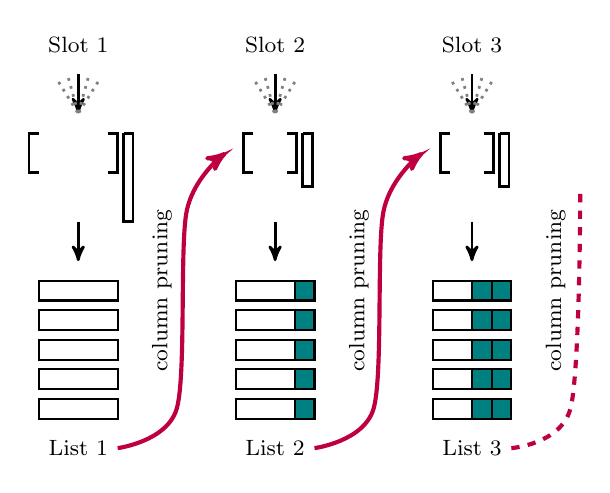
\begin{tikzpicture}
[font=\footnotesize, draw=black, line width=0.75pt,>=stealth',
sub0/.style={rectangle, draw, inner sep=0pt, minimum width=10mm, minimum height=2.5mm},
parity/.style={rectangle, draw, fill=teal, inner sep=0pt, minimum size=2.5mm}]

\node (cs1) at (0.00,6.125) {Slot~1};
\node (cs2) at (2.50,6.125) {Slot~2};
\node (cs3) at (5.00,6.125) {Slot~3};

\foreach \v in {0.00,2.50,5.00} {
  \draw[->, line width=1pt]  (\v,3.875) -- (\v,3.375);
  \draw[->, line width=1pt]  (\v,5.75) -- (\v,5.25);
  \draw[dotted, line width=1pt, draw=gray]  (\v-0.25,5.65) -- (\v,5.25);
  \draw[dotted, line width=1pt, draw=gray]  (\v-0.125,5.7) -- (\v,5.25);
  \draw[dotted, line width=1pt, draw=gray]  (\v+0.125,5.7) -- (\v,5.25);
  \draw[dotted, line width=1pt, draw=gray]  (\v+0.25,5.65) -- (\v,5.25);
}

\foreach \v in {0.00} {
  \draw[line width=1pt] (\v-0.5,5) -- (\v-0.625,5) -- (\v-0.625,4.5) -- (\v-0.5,4.5);
  \draw[line width=1pt] (\v+0.375,5) -- (\v+0.5,5) -- (\v+0.5,4.5) -- (\v+0.375,4.5);
  \draw[line width=1pt] (\v+0.575,5) -- (\v+0.575,3.875) -- (\v+0.695,3.875) -- (\v+0.695,5) -- (\v+0.575,5);
}

\foreach \v in {2.50,5.00} {
  \draw[line width=1pt] (\v-0.275,5) -- (\v-0.4,5) -- (\v-0.4,4.5) -- (\v-0.275,4.5);
  \draw[line width=1pt] (\v+0.15,5) -- (\v+0.275,5) -- (\v+0.275,4.5) -- (\v+0.15,4.5);
  \draw[line width=1pt] (\v+0.35,5) -- (\v+0.35,4.325) -- (\v+0.47,4.325) -- (\v+0.47,5) -- (\v+0.35,5);
}

\foreach \p/\c in {3.00/1, 2.625/2, 2.25/3, 1.875/4, 1.5/5} {
  \node[sub0] (subcs1\c) at (0.0,\p) {};
  \node[sub0] (subcs2\c) at (2.50,\p) {};
  \node[parity] (parity0\c) at (2.875,\p) {};
  \node[sub0] (subcs3\c) at (5.00,\p) {};
  \node[parity] (parity1\c) at (5.125,\p) {};
  \node[parity] (parity2\c) at (5.375,\p) {};
}

\node (list1) at (0.00,1) {List~1};
\node (list2) at (2.50,1) {List~2};
\node (list3) at (5.00,1) {List~3};

\draw [line width=1.5pt,color=purple,->] plot[smooth, tension=.5] coordinates {(0.5,1) (1.25,1.5) (1.375,4) (1.875,4.75)};
\draw [line width=1.5pt,color=purple,->] plot[smooth, tension=.5] coordinates {(3.0,1) (3.75,1.5) (3.875,4) (4.375,4.75)};
\draw [line width=1.5pt,color=purple,dashed] plot[smooth, tension=.5] coordinates {(5.5,1) (6.25,1.5) (6.375,4.25)};

\node[rotate=90] (prune1) at (1.0625,3) {column pruning};
\node[rotate=90] (prune2) at (3.5625,3) {column pruning};
\node[rotate=90] (prune3) at (6.0625,3) {column pruning};
\end{tikzpicture}

\end{center}
\vfill
\begin{itemize}
\item Active partial paths determine possible parity patterns
\item Admissible indices for next slot determined by possible parities
\item Inadmissible columns can be pruned before CS algorithm
\end{itemize}
\end{frame}

% % % % % % % % % % % % % % % % % % % %

%\begin{frame}
%\frametitle{Coded Compressive Sensing -- Dimensionality Reduction}
%\centerline{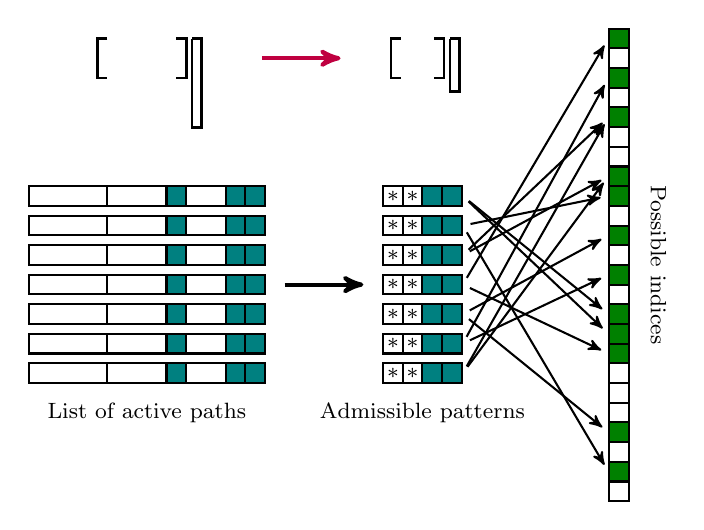
\begin{tikzpicture}
[font=\footnotesize, draw=black, line width=0.75pt,>=stealth',
sub0/.style={rectangle, draw, inner sep=0pt, minimum width=10mm, minimum height=2.5mm},
parity/.style={rectangle, draw, fill=teal, inner sep=0pt, minimum size=2.5mm},
star/.style={rectangle, draw, inner sep=0pt, minimum size=2.5mm},
symbol0/.style={rectangle, draw, fill=white, inner sep=0pt, minimum size=2.5mm},
symbol1/.style={rectangle, draw, fill=green!50!black, inner sep=0pt, minimum size=2.5mm}]

\foreach \v in {1.00} {
  \draw[line width=1pt] (\v-0.5,5) -- (\v-0.625,5) -- (\v-0.625,4.5) -- (\v-0.5,4.5);
  \draw[line width=1pt] (\v+0.375,5) -- (\v+0.5,5) -- (\v+0.5,4.5) -- (\v+0.375,4.5);
  \draw[line width=1pt] (\v+0.575,5) -- (\v+0.575,3.875) -- (\v+0.695,3.875) -- (\v+0.695,5) -- (\v+0.575,5);
}
\draw [line width=1.5pt,color=purple,->] (2.46,4.75) -- (3.46,4.75);

\foreach \v in {4.50} {
  \draw[line width=1pt] (\v-0.275,5) -- (\v-0.4,5) -- (\v-0.4,4.5) -- (\v-0.275,4.5);
  \draw[line width=1pt] (\v+0.15,5) -- (\v+0.275,5) -- (\v+0.275,4.5) -- (\v+0.15,4.5);
  \draw[line width=1pt] (\v+0.35,5) -- (\v+0.35,4.325) -- (\v+0.47,4.325) -- (\v+0.47,5) -- (\v+0.35,5);
}


\foreach \p/\c in {3.00/1, 2.625/2, 2.25/3, 1.875/4, 1.5/5, 1.125/6, 0.75/7} {
  \node[sub0] (subcs1\c) at (0.0,\p) {};
  \node[sub0] (subcs2\c) at (1.0,\p) {};
  \node[parity] (parity0\c) at (1.375,\p) {};
  \node[sub0] (subcs3\c) at (2.00,\p) {};
  \node[parity] (parity1\c) at (2.125,\p) {};
  \node[parity] (parity2\c) at (2.375,\p) {};
}
\node (list) at (1.00,0.25) {List of active paths};
\draw [line width=1.5pt,->] (2.75,1.875) -- (3.75,1.875);

\foreach \p/\c in {3.00/1, 2.625/2, 2.25/3, 1.875/4, 1.5/5, 1.125/6, 0.75/7} {
  \node[sub0] (subcs4\c) at (4.50,\p) {};
  \node[star] (star0\c) at (4.125,\p) {$\ast$};
  \node[star] (star1\c) at (4.375,\p) {$\ast$};
  \node[parity] (parity3\c) at (4.625,\p) {};
  \node[parity] (parity4\c) at (4.875,\p) {};
}
\node (patterns) at (4.50,0.25) {Admissible patterns};

\node[symbol0] (s01) at (7,-0.75) {};
\node[symbol1] (s02) at (7,-0.50) {};
\node[symbol0] (s03) at (7,-0.25) {};
\node[symbol1] (s04) at (7,0.00) {};
\node[symbol0] (s05) at (7,0.25) {};
\node[symbol0] (s06) at (7,0.50) {};
\node[symbol0] (s07) at (7,0.75) {};
\node[symbol1] (s08) at (7,1.00) {};
\node[symbol1] (s09) at (7,1.25) {};
\node[symbol1] (s10) at (7,1.50) {};
\node[symbol0] (s11) at (7,1.75) {};
\node[symbol1] (s12) at (7,2.00) {};
\node[symbol0] (s13) at (7,2.25) {};
\node[symbol1] (s14) at (7,2.50) {};
\node[symbol0] (s15) at (7,2.75) {};
\node[symbol1] (s16) at (7,3.00) {};
\node[symbol1] (s17) at (7,3.25) {};
\node[symbol0] (s18) at (7,3.50) {};
\node[symbol0] (s19) at (7,3.75) {};
\node[symbol1] (s20) at (7,4.00) {};
\node[symbol0] (s21) at (7,4.25) {};
\node[symbol1] (s22) at (7,4.50) {};
\node[symbol0] (s23) at (7,4.75) {};
\node[symbol1] (s24) at (7,5.00) {};
\node[rotate=-90] (indices) at (7.5,2.125) {Possible indices};

\draw[->,shorten <=1mm,shorten >=1mm]  (parity42.east) -- (s02.west);
\draw[->,shorten <=1mm,shorten >=1mm]  (parity45.east) -- (s04.west);
\draw[->,shorten <=1mm,shorten >=1mm]  (parity44.east) -- (s08.west);
\draw[->,shorten <=1mm,shorten >=1mm]  (parity41.east) -- (s09.west);
\draw[->,shorten <=1mm,shorten >=1mm]  (parity41.east) -- (s10.west);
\draw[->,shorten <=1mm,shorten >=1mm]  (parity46.east) -- (s12.west);
\draw[->,shorten <=1mm,shorten >=1mm]  (parity45.east) -- (s14.west);
\draw[->,shorten <=1mm,shorten >=1mm]  (parity42.east) -- (s16.west);
\draw[->,shorten <=1mm,shorten >=1mm]  (parity43.east) -- (s17.west);
\draw[->,shorten <=1mm,shorten >=1mm]  (parity43.east) -- (s20.west);
\draw[->,shorten <=1mm,shorten >=1mm]  (parity46.east) -- (s22.west);
\draw[->,shorten <=1mm,shorten >=1mm]  (parity44.east) -- (s24.west);
\draw[->,shorten <=1mm,shorten >=1mm]  (parity47.east) -- (s17.west);
\draw[->,shorten <=1mm,shorten >=1mm]  (parity47.east) -- (s20.west);

\end{tikzpicture}
}
%\begin{itemize}
%\item Every surviving path produces parity pattern
%\item Only fragments with these pattern can appear in subsequent slot
%\item On average, there are $K (1 + \mathrm{E}[P_{\ell}])$ possibilities parity patterns
%\end{itemize}
%\end{frame}

% % % % % % % % % % % % % % % % % % % %

\begin{frame}
\frametitle{Coded Compressive Sensing with Column Pruning}
\begin{center}
\input{Figures-CCS/eCCS3}
\end{center}
\vfill
\begin{itemize}
\item For $K$ small, width of sensing matrix is greatly reduced
\item Actual sensing matrix is determined dynamically at run time
\item Complexity of CS algorithm becomes much smaller
\end{itemize}
\end{frame}

% % % % % % % % % % % % % % % % % % % %

\begin{frame}
\frametitle{Expected Column Reduction Ratio}
\begin{columns}
\column{0.6\textwidth}
  \centerline{\scalebox{0.9}{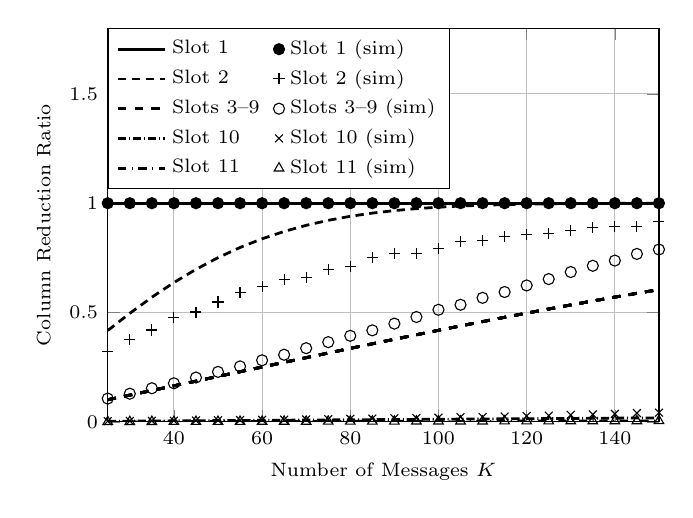
\begin{tikzpicture}

\begin{axis}[%
font=\scriptsize,
width=7cm,
height=5cm,
scale only axis,
xmin=25,
xmax=150,
xlabel={Number of Messages $K$},
xmajorgrids,
ymin=0,
ymax=1.8,
ylabel={Column Reduction Ratio},
ylabel near ticks,
ymajorgrids,
legend columns=2, 
legend style={at={(0,1)},anchor=north west,legend cell align=left,
/tikz/column 2/.style={column sep=3pt}}
]

\addplot [color=black,solid,line width=1.0pt]
  coordinates {
(25, 1.00000) (30, 1.00000) (35, 1.00000) (40, 1.00000) (45, 1.00000) (50, 1.00000) (55, 1.00000) (60, 1.00000) (65, 1.00000) (70, 1.00000) (75, 1.00000) (80, 1.00000) (85, 1.00000) (90, 1.00000) (95, 1.00000) (100, 1.00000) (105, 1.00000) (110, 1.00000) (115, 1.00000) (120, 1.00000) (125, 1.00000) (130, 1.00000) (135, 1.00000) (140, 1.00000) (145, 1.00000) (150, 1.00000)
};
\addlegendentry{Slot 1};

\addplot [only marks,mark=*]
  coordinates {
(25, 1.00000) (30, 1.00000) (35, 1.00000) (40, 1.00000) (45, 1.00000) (50, 1.00000) (55, 1.00000) (60, 1.00000) (65, 1.00000) (70, 1.00000) (75, 1.00000) (80, 1.00000) (85, 1.00000) (90, 1.00000) (95, 1.00000) (100, 1.00000) (105, 1.00000) (110, 1.00000) (115, 1.00000) (120, 1.00000) (125, 1.00000) (130, 1.00000) (135, 1.00000) (140, 1.00000) (145, 1.00000) (150, 1.00000)
};
\addlegendentry{Slot 1 (sim)};

\addplot [color=black,densely dashed,line width=1.0pt]
  coordinates {
(25, 0.41804) (30, 0.49668) (35, 0.57002) (40, 0.63716) (45, 0.69757) (50, 0.75100) (55, 0.79749) (60, 0.83732) (65, 0.87092) (70, 0.89882) (75, 0.92167) (80, 0.94010) (85, 0.95475) (90, 0.96624) (95, 0.97511) (100, 0.98188) (105, 0.98697) (110, 0.99075) (115, 0.99351) (120, 0.99550) (125, 0.99692) (130, 0.99792) (135, 0.99861) (140, 0.99908) (145, 0.99940) (150, 0.99961)
};
%curve below is generate using the PMF of #erroneous paths
%coordinates {
%(25, 0.3254) (30, 0.3765) (35, 0.4237) (40, 0.4674) (45, 0.5077) (50, 0.5450) (55, 0.5794) (60, 0.6113) (65, 0.6407) (70, 0.6679) (75, 0.6931) (80, 0.7163) (85, 0.7378) (90, 0.7576) (95, 0.7760) (100, 0.7930) (105, 0.8086) (110, 0.8231) (115, 0.8365) (120, 0.8489) (125, 0.8603) (130, 0.8709) (135, 0.8807) (140, 0.8897) (145, 0.8981) (150, 0.9058)
%};
\addlegendentry{Slot 2};

\addplot [only marks,mark=+]
  coordinates {
(25,0.3218750) (30,0.3773437) (35,4.203125e-01) (40,4.765625e-01) (45,5.023437e-01) (50,5.484375e-01) (55,5.898438e-01) (60,6.171875e-01) (65,6.515625e-01)
(70,6.585937e-01) (75,6.953125e-01) (80,7.117187e-01) (85,7.523437e-01) (90,7.695313e-01) (95,7.703125e-01)
(100,7.929688e-01) (105,8.250000e-01) (110,8.296875e-01) (115,8.484375e-01) (120,8.578125e-01)(125,8.609e-01)(130,8.734e-01)(135,8.8906e-01)(140,8.9218e-01)(145,8.9375e-01)(150,9.1562e-01)

};
\addlegendentry{Slot 2 (sim)};

\addplot [color=black,dashed,line width=1.0pt]
  coordinates {
(25, 0.10149) (30, 0.12253) (35, 0.14374) (40, 0.16507) (45, 0.18649) (50, 0.20797) (55, 0.22947) (60, 0.25095) (65, 0.27240) (70, 0.29377) (75, 0.31504) (80, 0.33617) (85, 0.35715) (90, 0.37794) (95, 0.39851) (100, 0.41885) (105, 0.43893) (110, 0.45873) (115, 0.47823) (120, 0.49741) (125, 0.51626) (130, 0.53476) (135, 0.55289) (140, 0.57064) (145, 0.58800) (150, 0.60497)
};
%coordinates {
%(25,0.0932) (30,0.1108)    (35,0.1280)    (40,0.1449)    (45,0.1615)    (50,0.1777)    (55,0.1937)    (60,0.2093)    (65,0.2246)    (70,0.2396)    (75,0.2544)  (80,0.2688)    (85,0.2830)    (90,0.2969)    (95,0.3105)    (100,0.3239)    (105,0.3370)    (110,0.3498)    (115,0.3624)    (120,0.3748)    (125,0.3869)    (130,0.3988) (135,0.4104)    (140,0.4219)    (145,0.4331)    (150,0.4441) 
%};
\addlegendentry{Slots 3--9};

\addplot [only marks,mark=o]
  coordinates {(25,1.067801e-01) (30,1.290179e-01) (35,1.539342e-01) (40,1.766462e-01) (45,2.029297e-01) (50,2.287109e-01) (55,2.539342e-01) (60,2.817243e-01) (65,3.071429e-01)
(70,3.371094e-01) (75,3.647879e-01) (80,3.937221e-01) (85,4.186663e-01) (90,4.494420e-01) (95,4.797433e-01)
(100,5.127511e-01) (105,5.356027e-01) (110,5.672991e-01) (115,5.939732e-01) (120,6.239955e-01)(125,6.5306e-01)(130,6.8526e-01)(135,7.1395e-01)(140,7.3766e-01)(145,7.6813e-01)(150,7.8825e-01)
};
\addlegendentry{Slots 3--9 (sim)};

\addplot [color=black,densely dashdotted,line width=1.0pt]
  coordinates {
(25, 0.00306) (30, 0.00367) (35, 0.00428) (40, 0.00489) (45, 0.00551) (50, 0.00612) (55, 0.00674) (60, 0.00735) (65, 0.00797) (70, 0.00858) (75, 0.00920) (80, 0.00981) (85, 0.01043) (90, 0.01104) (95, 0.01166) (100, 0.01228) (105, 0.01290) (110, 0.01352) (115, 0.01413) (120, 0.01475) (125, 0.01537) (130, 0.01599) (135, 0.01661) (140, 0.01723) (145, 0.01785) (150, 0.01847)
};
%coordinates {
% (25,0.0030)    (30,0.0037)    (35,0.0043)    (40,0.0049)    (45,0.0055)    (50,0.0061)    (55,0.0067)    (60,0.0073)    (65,0.0079)    (70,0.0085)    (75,0.0091)
%    (80,0.0097)    (85,0.0103)    (90,0.0109)    (95,0.0115)    (100,0.0121)    (105,0.0127)    (110,0.0133)    (115,0.0139)    (120,0.0145)    (125,0.0151)    (130,0.0157)  
%    (135,0.0163)    (140,0.0169)    (145,0.0175)    (150,0.0181)  
%};
\addlegendentry{Slot 10};

\addplot [only marks,mark=x]
  coordinates {(25,3.332520e-03) (30,4.180908e-03) (35,4.901123e-03) (40,5.511475e-03) (45,6.542969e-03) (50,7.434082e-03) (55,8.605957e-03) (60,9.436035e-03) (65,1.044312e-02)
 (70,1.149292e-02) (75,1.278687e-02) (80,1.430054e-02) (85,1.522217e-02) (90,1.674194e-02) (95,1.811523e-02)
(100,1.921997e-02) (105,2.165527e-02) (110,2.257080e-02) (115,2.467041e-02) (120,2.714844e-02)(125,2.8845e-02)(130,3.2532e-02)(135,3.4167e-02)(140,3.6804e-02)(145,4.0258e-02)(150,4.2333e-02)
};
\addlegendentry{Slot 10 (sim)};

\addplot [color=black,dashdotted,line width=1.0pt]
  coordinates {
(25, 0.00076) (30, 0.00092) (35, 0.00107) (40, 0.00122) (45, 0.00137) (50, 0.00153) (55, 0.00168) (60, 0.00183) (65, 0.00199) (70, 0.00214) (75, 0.00229) (80, 0.00244) (85, 0.00260) (90, 0.00275) (95, 0.00290) (100, 0.00306) (105, 0.00321) (110, 0.00336) (115, 0.00352) (120, 0.00367) (125, 0.00382) (130, 0.00398) (135, 0.00413) (140, 0.00428) (145, 0.00443) (150, 0.00459)
};
%coordinates{
%(25,0.0008)    (30,0.0009)    (35,0.0011)    (40,0.0014)    (45,0.0015)    (50,0.0017)    (55,0.0018)    (60,0.0020)    (65,0.0021)    (70,0.0023)    (75,0.0024)
 %   (80,0.0026)    (85,0.0028)    (90,0.0029)    (95,0.0031)    (100,0.0032)    (105,0.0034)    (110,0.0035)    (115,0.0037)    (120,0.0038)    (125,0.0040)    (130,0.0041)  
  %  (135,0.0043)    (140,0.0044)    (145,0.0046)    (150,0.0047)
%}
\addlegendentry{Slot 11};

\addplot [only marks,mark=triangle]
  coordinates {(25,7.644653e-04) (30,9.170532e-04) (35,1.072693e-03) (40,1.228333e-03) (45,1.380920e-03) (50,1.538086e-03) (55,1.689148e-03) (60,1.841736e-03) (65,1.997375e-03)
 (70,2.151489e-03) (75,2.307129e-03) (80,2.476501e-03) (85,2.627563e-03) (90,2.786255e-03) (95,2.940369e-03)
(100,3.100586e-03) (105,3.288269e-03) (110,3.399658e-03) (115,3.573608e-03) (120,3.771973e-03)(125,3.9337e-03)(130,4.0740e-3)(135,4.2205e-03)(140,4.3854e-03)(145,4.5380e-03)(150,4.7241e-03)
};
\addlegendentry{Slot 11 (sim)};

\addplot [color=black,dashed,line width=1.0pt]
  coordinates {
(25, 0.10149) (30, 0.12253) (35, 0.14374) (40, 0.16507) (45, 0.18649) (50, 0.20797) (55, 0.22947) (60, 0.25095) (65, 0.27240) (70, 0.29377) (75, 0.31504) (80, 0.33617) (85, 0.35715) (90, 0.37794) (95, 0.39851) (100, 0.41885) (105, 0.43893) (110, 0.45873) (115, 0.47823) (120, 0.49741) (125, 0.51626) (130, 0.53476) (135, 0.55289) (140, 0.57064) (145, 0.58800) (150, 0.60497)
};

\addplot [color=black,dashed,line width=1.0pt]
  coordinates {
(25, 0.10149) (30, 0.12253) (35, 0.14374) (40, 0.16507) (45, 0.18649) (50, 0.20797) (55, 0.22947) (60, 0.25095) (65, 0.27240) (70, 0.29377) (75, 0.31504) (80, 0.33617) (85, 0.35715) (90, 0.37794) (95, 0.39851) (100, 0.41885) (105, 0.43893) (110, 0.45873) (115, 0.47823) (120, 0.49741) (125, 0.51626) (130, 0.53476) (135, 0.55289) (140, 0.57064) (145, 0.58800) (150, 0.60497)
};

\addplot [color=black,dashed,line width=1.0pt]
  coordinates {
(25, 0.10149) (30, 0.12253) (35, 0.14374) (40, 0.16507) (45, 0.18649) (50, 0.20797) (55, 0.22947) (60, 0.25095) (65, 0.27240) (70, 0.29377) (75, 0.31504) (80, 0.33617) (85, 0.35715) (90, 0.37794) (95, 0.39851) (100, 0.41885) (105, 0.43893) (110, 0.45873) (115, 0.47823) (120, 0.49741) (125, 0.51626) (130, 0.53476) (135, 0.55289) (140, 0.57064) (145, 0.58800) (150, 0.60497)
};

\addplot [color=black,dashed,line width=1.0pt]
  coordinates {
(25, 0.10149) (30, 0.12253) (35, 0.14374) (40, 0.16507) (45, 0.18649) (50, 0.20797) (55, 0.22947) (60, 0.25095) (65, 0.27240) (70, 0.29377) (75, 0.31504) (80, 0.33617) (85, 0.35715) (90, 0.37794) (95, 0.39851) (100, 0.41885) (105, 0.43893) (110, 0.45873) (115, 0.47823) (120, 0.49741) (125, 0.51626) (130, 0.53476) (135, 0.55289) (140, 0.57064) (145, 0.58800) (150, 0.60497)
};

\addplot [color=black,dashed,line width=1.0pt]
  coordinates {
(25, 0.10149) (30, 0.12253) (35, 0.14374) (40, 0.16507) (45, 0.18649) (50, 0.20797) (55, 0.22947) (60, 0.25095) (65, 0.27240) (70, 0.29377) (75, 0.31504) (80, 0.33617) (85, 0.35715) (90, 0.37794) (95, 0.39851) (100, 0.41885) (105, 0.43893) (110, 0.45873) (115, 0.47823) (120, 0.49741) (125, 0.51626) (130, 0.53476) (135, 0.55289) (140, 0.57064) (145, 0.58800) (150, 0.60497)
};

\addplot [color=black,dashed,line width=1.0pt]
  coordinates {
(25, 0.10149) (30, 0.12253) (35, 0.14374) (40, 0.16507) (45, 0.18649) (50, 0.20797) (55, 0.22947) (60, 0.25095) (65, 0.27240) (70, 0.29377) (75, 0.31504) (80, 0.33617) (85, 0.35715) (90, 0.37794) (95, 0.39851) (100, 0.41885) (105, 0.43893) (110, 0.45873) (115, 0.47823) (120, 0.49741) (125, 0.51626) (130, 0.53476) (135, 0.55289) (140, 0.57064) (145, 0.58800) (150, 0.60497)
};
\end{axis}

\end{tikzpicture}
}}
\column{0.2\textwidth}
  \centerline{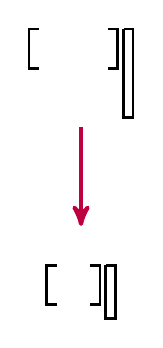
\begin{tikzpicture}
[font=\footnotesize, draw=black, line width=0.75pt,>=stealth']

\foreach \v in {1.00} {
  \draw[line width=1pt] (\v-0.5,5) -- (\v-0.625,5) -- (\v-0.625,4.5) -- (\v-0.5,4.5);
  \draw[line width=1pt] (\v+0.375,5) -- (\v+0.5,5) -- (\v+0.5,4.5) -- (\v+0.375,4.5);
  \draw[line width=1pt] (\v+0.575,5) -- (\v+0.575,3.875) -- (\v+0.695,3.875) -- (\v+0.695,5) -- (\v+0.575,5);
}

\draw [line width=1.5pt,color=purple,->] (1.035,3.75) -- (1.035,2.5);

\foreach \v in {1} {
  \draw[line width=1pt] (\v-0.275,2) -- (\v-0.4,2) -- (\v-0.4,1.5) -- (\v-0.275,1.5);
  \draw[line width=1pt] (\v+0.15,2) -- (\v+0.275,2) -- (\v+0.275,1.5) -- (\v+0.15,1.5);
  \draw[line width=1pt] (\v+0.35,2) -- (\v+0.35,1.325) -- (\v+0.47,1.325) -- (\v+0.47,2) -- (\v+0.35,2);
}

\end{tikzpicture}
}
\end{columns}
\begin{itemize}
\item Parity allocation parameters, with $w_{\ell} + p_{\ell} = 15$,
\begin{equation*}
(p_1, p_2, \ldots, p_{10}) = (6, 8, 8, 8, 8, 8, 8, 8, 13, 15)
\end{equation*}
\item Pruning is more pronounced at later stages
\item Effective width of sensing matrix is greatly reduced
\end{itemize}
\end{frame}

% % % % % % % % % % % % % % % % % % % %

\begin{frame}
\frametitle{Leveraging CCS Framework}
% % % % %
\begin{center}
\begin{tikzpicture}
  \node[scope fading=south] (image) at (0,0) {\includegraphics[width=4in]{Figures-CCS/CCS-MIMO.png}};
\end{tikzpicture}
\end{center}
  \begin{itemize}
  \item Activity detection in random access
  \item Massive MIMO Receiver
  \end{itemize}
\end{frame}

% % % % % % % % % % % % % % % % % % % %

\begin{frame}
\frametitle{Massive MIMO-URA}
\begin{center}
\scalebox{0.75}{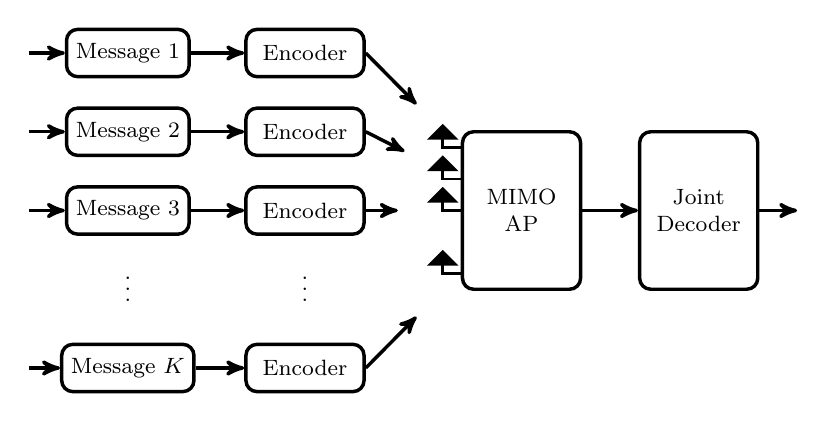
\begin{tikzpicture}
  [
  font=\footnotesize, draw=black, >=stealth', line width=1.25pt,
  channel/.style={rectangle, minimum height=20mm, minimum width=15mm, draw=black, rounded corners},
  encoder/.style={rectangle, minimum height=6mm, minimum width=15mm, draw=black, rounded corners},
  decoder/.style={rectangle, minimum height=20mm, minimum width=15mm, draw=black, rounded corners},
  message/.style={rectangle, minimum height=6mm, minimum width=15mm, draw=black, rounded corners}
  ]

\foreach \e in {1,2,3,5} {
  \node[encoder] (e\e) at (2.25,3-\e) {Encoder};
}

\foreach \m in {1,2,3} {
  \node[message] (m\m) at (0.0,3-\m) {Message~${\m}$}
  edge[->] (e\m);
  \draw[<-] (m\m) -- (-1.25,3-\m);
}

\foreach \m in {5} {
  \node[message] (m\m) at (0.0,3-\m) {Message~$K$}
  edge[->] (e\m);
  \draw[<-] (m\m) -- (-1.25,3-\m);
}

\node at (0,-0.9) {$\vdots$};
\node at (2.25,-0.9) {$\vdots$};

\node[channel,align=center] (channel) at (5,0) {MIMO\\AP};
\node[decoder,align=center] (decoder) at (7.25,0) {Joint\\Decoder};
\draw[->] (channel) -- (decoder);


\draw[->] (decoder.east) -- (8.5,0);

\draw [line width=1pt,color=black,-triangle 90] plot[smooth, tension=0] coordinates {(4.25,0.8)(4,0.8)(4,1.1)};
\draw [line width=1pt,color=black,-triangle 90] plot[smooth, tension=0] coordinates {(4.25,0.4)(4,0.4)(4,0.7)};
\draw [line width=1pt,color=black,-triangle 90] plot[smooth, tension=0] coordinates {(4.25,0)(4,0)(4,0.3)};
\draw [line width=1pt,color=black,-triangle 90] plot[smooth, tension=0] coordinates {(4.25,-0.8)(4,-0.8)(4,-0.5)};

\draw[->,shorten >=8mm] (e1.east) -- (channel);
\draw[->,shorten >=8mm] (e2.east) -- (channel);
\draw[->,shorten >=8mm] (e3.east) -- (channel);
\draw[->,shorten >=8mm] (e5.east) -- (channel);

\end{tikzpicture}
}
%\scalebox{0.75}{\input{Figures-MAC/uncoordinated}}
\end{center}
\vfill
\begin{block}{Signal model}
\begin{itemize}
\item Signal received at time instant~$t$ with slot~$\ell$
\begin{equation*}
\yv(t,\ell) =
\textstyle \sum_{k=1}^K \xv_k(t,\ell) \mathbf{h}_k(\ell) + \zv(t,\ell)
%,~\xv_k = f(\wv_k) 
\end{equation*}
\item Number of receive antennas $M \gg 1$
\item Block fading -- channel does not change within CCS slot
\item Spatial correlation negligible -- $\mathbf{h}_k(\ell) \sim \mathcal{CN}(0,\mathbf{I}_M)$
\end{itemize}
\end{block}
\end{frame}

% % % % % % % % % % % % % % % % % % % %

\begin{frame}
\frametitle{Multiple Measurement Vector -- CS Interpretation}
% % % % %
\centerline{\definecolor{mycolor6}{rgb}{0.74902,0.00000,0.74902}%
\definecolor{mycolor7}{rgb}{0.87059,0.00000,0.49020}%
\definecolor{mycolor8}{rgb}{0.49020,0.00000,0.87059}%

\begin{tikzpicture}
[draw=black, line width=0.75pt,
entry0/.style={rectangle, draw, fill=white, inner sep=0pt, minimum size=2.5mm},
entry1/.style={rectangle, draw, fill=gray, inner sep=0pt, minimum size=2.5mm},
entry2/.style={rectangle, draw, fill=gray!50, inner sep=0pt, minimum size=2.5mm},
entry00/.style={rectangle, draw, fill=white, inner sep=0pt, minimum size=2.5mm},
entry11/.style={rectangle, draw, fill=gray!90, inner sep=0pt, minimum size=2.5mm},
symbol0/.style={rectangle, draw, fill=white, inner sep=0pt, minimum size=2.5mm},
symbol1/.style={rectangle, draw, fill=blue!50, inner sep=0pt, minimum size=2.5mm},
symbol2/.style={rectangle, draw, fill=blue, inner sep=0pt, minimum size=2.5mm},
symbol3/.style={rectangle, draw, fill=red!75, inner sep=0pt, minimum size=2.5mm},
symbol4/.style={rectangle, draw, fill=red!50, inner sep=0pt, minimum size=2.5mm},
symbol5/.style={rectangle, draw, fill=mycolor6, inner sep=0pt, minimum size=2.5mm},
symbol6/.style={rectangle, draw, fill=mycolor7, inner sep=0pt, minimum size=2.5mm},
symbol7/.style={rectangle, draw, fill=mycolor8, inner sep=0pt, minimum size=2.5mm}]

\node[entry0] (m0011) at (-0.50,1.50) {};
\node[entry1] (m0011) at (-0.25,1.50) {};
\node[entry0] (m0006) at (0.00,1.50) {};
\node[entry1] (m0106) at (0.25,1.50) {};
\node[entry00] (m0206) at (0.50,1.50) {};
\node[entry0] (m0306) at (0.75,1.50) {};
\node[entry0] (m0406) at (1.00,1.50) {};
\node[entry0] (m0506) at (1.25,1.50) {};
\node[entry00] (m0606) at (1.50,1.50) {};
\node[entry0] (m0706) at (1.75,1.50) {};
\node[entry0] (m0806) at (2.00,1.50) {};
\node[entry0] (m0906) at (2.25,1.50) {};

\node[entry0] (m0011) at (-0.50,1.75) {};
\node[entry0] (m0011) at (-0.25,1.75) {};
\node[entry0] (m0007) at (0.00,1.75) {};
\node[entry0] (m0107) at (0.25,1.75) {};
\node[entry00] (m0207) at (0.50,1.75) {};
\node[entry1] (m0307) at (0.75,1.75) {};
\node[entry0] (m0407) at (1.00,1.75) {};
\node[entry0] (m0507) at (1.25,1.75) {};
\node[entry00] (m0607) at (1.50,1.75) {};
\node[entry1] (m0707) at (1.75,1.75) {};
\node[entry1] (m0807) at (2.00,1.75) {};
\node[entry0] (m0907) at (2.25,1.75) {};

\node[entry00] (m0011) at (-0.50,2.00) {};
\node[entry1] (m0011) at (-0.25,2.00) {};
\node[entry0] (m0008) at (0.00,2.00) {};
\node[entry1] (m0108) at (0.25,2.00) {};
\node[entry00] (m0208) at (0.50,2.00) {};
\node[entry0] (m0308) at (0.75,2.00) {};
\node[entry0] (m0408) at (1.00,2.00) {};
\node[entry1] (m0508) at (1.25,2.00) {};
\node[entry00] (m0608) at (1.50,2.00) {};
\node[entry1] (m0708) at (1.75,2.00) {};
\node[entry0] (m0808) at (2.00,2.00) {};
\node[entry1] (m0908) at (2.25,2.00) {};

\node[entry0] (m0011) at (-0.5,2.25) {};
\node[entry0] (m0011) at (-0.25,2.25) {};
\node[entry0] (m0009) at (0.00,2.25) {};
\node[entry0] (m0109) at (0.25,2.25) {};
\node[entry11] (m0209) at (0.50,2.25) {};
\node[entry0] (m0309) at (0.75,2.25) {};
\node[entry1] (m0409) at (1.00,2.25) {};
\node[entry0] (m0509) at (1.25,2.25) {};
\node[entry00] (m0609) at (1.50,2.25) {};
\node[entry1] (m0709) at (1.75,2.25) {};
\node[entry0] (m0809) at (2.00,2.25) {};
\node[entry0] (m0909) at (2.25,2.25) {};


\node[entry1] (m0011) at (-0.5,2.5) {};
\node[entry0] (m0011) at (-0.25,2.5) {};
\node[entry1] (m0010) at (0.00,2.50) {};
\node[entry0] (m0110) at (0.25,2.50) {};
\node[entry00] (m0210) at (0.50,2.50) {};
\node[entry0] (m0310) at (0.75,2.50) {};
\node[entry0] (m0410) at (1.00,2.50) {};
\node[entry1] (m0510) at (1.25,2.50) {};
\node[entry11] (m0610) at (1.50,2.50) {};
\node[entry1] (m0710) at (1.75,2.50) {};
\node[entry0] (m0810) at (2.00,2.50) {};
\node[entry0] (m0910) at (2.25,2.50) {};

\node[entry11] (m0011) at (-0.5,2.75) {};
\node[entry0] (m0011) at (-0.25,2.75) {};
\node[entry0] (m0011) at (0.00,2.75) {};
\node[entry0] (m0111) at (0.25,2.75) {};
\node[entry00] (m0211) at (0.50,2.75) {};
\node[entry0] (m0311) at (0.75,2.75) {};
\node[entry0] (m0411) at (1.00,2.75) {};
\node[entry0] (m0511) at (1.25,2.75) {};
\node[entry11] (m0611) at (1.50,2.75) {};
\node[entry0] (m0711) at (1.75,2.75) {};
\node[entry0] (m0811) at (2.00,2.75) {};
\node[entry0] (m0911) at (2.25,2.75) {};

\node[symbol2] (g0000) at (2.75,2.75) {};
\node[entry0] (g0001) at (3,2.75) {};
\node[entry0] (g0002) at (3.25,2.75) {};
\node[entry0] (g0003) at (3.5,2.75) {};
\node[entry0] (g0004) at (3.75,2.75) {};
\node[entry0] (g0005) at (4.00,2.75) {};
\node[entry0] (g0006) at (4.25,2.75) {};
\node[entry0] (g0007) at (4.5,2.75) {};
\node[entry0] (g0008) at (4.75,2.75) {};
\node[entry0] (g0009) at (5,2.75) {};
\node[entry0] (g00091) at (5.25,2.75) {};
\node[entry0] (g00092) at (5.5,2.75) {};

\node[entry0] (g0010) at (2.75,2.5) {};
\node[entry2] (g0011) at (3,2.5) {};
\node[entry0] (g0012) at (3.25,2.5) {};
\node[entry0] (g0013) at (3.5,2.5) {};
\node[entry0] (g0014) at (3.75,2.5) {};
\node[entry0] (g0015) at (4.00,2.5) {};
\node[entry0] (g0016) at (4.25,2.5) {};
\node[entry0] (g0017) at (4.5,2.5) {};
\node[entry0] (g0018) at (4.75,2.5) {};
\node[entry0] (g0019) at (5,2.5) {};
\node[entry0] (g00191) at (5.25,2.5) {};
\node[entry0] (g00192) at (5.5,2.5) {};

\node[entry0] (g0020) at (2.75,2.25) {};
\node[entry0] (g0021) at (3,2.25) {};
\node[symbol2] (g0022) at (3.25,2.25) {};
\node[entry0] (g0023) at (3.5,2.25) {};
\node[entry0] (g0024) at (3.75,2.25) {};
\node[entry0] (g0025) at (4.00,2.25) {};
\node[entry0] (g0026) at (4.25,2.25) {};
\node[entry0] (g0027) at (4.5,2.25) {};
\node[entry0] (g0028) at (4.75,2.25) {};
\node[entry0] (g0029) at (5,2.25) {};
\node[entry0] (g00291) at (5.25,2.25) {};
\node[entry0] (g00292) at (5.5,2.25) {};

\node[entry0] (g0030) at (2.75,2) {};
\node[entry0] (g0031) at (3,2) {};
\node[entry0] (g0032) at (3.25,2) {};
\node[entry2] (g0033) at (3.5,2) {};
\node[entry0] (g0034) at (3.75,2) {};
\node[entry0] (g0035) at (4.00,2) {};
\node[entry0] (g0036) at (4.25,2) {};
\node[entry0] (g0037) at (4.5,2) {};
\node[entry0] (g0038) at (4.75,2) {};
\node[entry0] (g0039) at (5,2) {};
\node[entry0] (g00391) at (5.25,2) {};
\node[entry0] (g00392) at (5.5,2) {};

\node[entry0] (g0040) at (2.75,1.75) {};
\node[entry0] (g0041) at (3,1.75) {};
\node[entry0] (g0042) at (3.25,1.75) {};
\node[entry0] (g0043) at (3.5,1.75) {};
\node[entry2] (g0044) at (3.75,1.75) {};
\node[entry0] (g0045) at (4.00,1.75) {};
\node[entry0] (g0046) at (4.25,1.75) {};
\node[entry0] (g0047) at (4.5,1.75) {};
\node[entry0] (g0048) at (4.75,1.75) {};
\node[entry0] (g0049) at (5,1.75) {};
\node[entry0] (g00491) at (5.25,1.75) {};
\node[entry0] (g00492) at (5.5,1.75) {};

\node[entry0] (g0050) at (2.75,1.5) {};
\node[entry0] (g0051) at (3,1.5) {};
\node[entry0] (g0052) at (3.25,1.5) {};
\node[entry0] (g0053) at (3.5,1.5) {};
\node[entry0] (g0054) at (3.75,1.5) {};
\node[entry2] (g0055) at (4.00,1.5) {};
\node[entry0] (g0056) at (4.25,1.5) {};
\node[entry0] (g0057) at (4.5,1.5) {};
\node[entry0] (g0058) at (4.75,1.5) {};
\node[entry0] (g0059) at (5,1.5) {};
\node[entry0] (g00591) at (5.25,1.5) {};
\node[entry0] (g00592) at (5.5,1.5) {};

\node[entry0] (g0060) at (2.75,1.25) {};
\node[entry0] (g0061) at (3,1.25) {};
\node[entry0] (g0062) at (3.25,1.25) {};
\node[entry0] (g0063) at (3.5,1.25) {};
\node[entry0] (g0064) at (3.75,1.25) {};
\node[entry0] (g0065) at (4.00,1.25) {};
\node[symbol2] (g0066) at (4.25,1.25) {};
\node[entry0] (g0067) at (4.5,1.25) {};
\node[entry0] (g0068) at (4.75,1.25) {};
\node[entry0] (g0069) at (5,1.25) {};
\node[entry0] (g00691) at (5.25,1.25) {};
\node[entry0] (g00692) at (5.5,1.25) {};

\node[entry0] (g0070) at (2.75,1) {};
\node[entry0] (g0071) at (3,1) {};
\node[entry0] (g0072) at (3.25,1) {};
\node[entry0] (g0073) at (3.5,1) {};
\node[entry0] (g0074) at (3.75,1) {};
\node[entry0] (g0075) at (4.00,1) {};
\node[entry0] (g0076) at (4.25,1) {};
\node[symbol2] (g0077) at (4.5,1) {};
\node[entry0] (g0078) at (4.75,1) {};
\node[entry0] (g0079) at (5,1) {};
\node[entry0] (g00791) at (5.25,1) {};
\node[entry0] (g00792) at (5.5,1) {};

\node[entry0] (g0080) at (2.75,0.75) {};
\node[entry0] (g0081) at (3,0.75) {};
\node[entry0] (g0082) at (3.25,0.75) {};
\node[entry0] (g0083) at (3.5,0.75) {};
\node[entry0] (g0084) at (3.75,0.75) {};
\node[entry0] (g0085) at (4.00,0.75) {};
\node[entry0] (g0086) at (4.25,0.75) {};
\node[entry0] (g0087) at (4.5,0.75) {};
\node[entry2] (g0088) at (4.75,0.75) {};
\node[entry0] (g0089) at (5,0.75) {};
\node[entry0] (g00891) at (5.25,0.75) {};
\node[entry0] (g00892) at (5.5,0.75) {};

\node[entry0] (g0090) at (2.75,0.5) {};
\node[entry0] (g0091) at (3,0.5) {};
\node[entry0] (g0092) at (3.25,0.5) {};
\node[entry0] (g0093) at (3.5,0.5) {};
\node[entry0] (g0094) at (3.75,0.5) {};
\node[entry0] (g0095) at (4.00,0.5) {};
\node[entry0] (g0096) at (4.25,0.5) {};
\node[entry0] (g0097) at (4.5,0.5) {};
\node[entry0] (g0098) at (4.75,0.5) {};
\node[entry2] (g0099) at (5,0.5) {};
\node[entry0] (g00991) at (5.25,0.5) {};
\node[entry0] (g00992) at (5.5,0.5) {};

\node[entry0] (g0090) at (2.75,0.25) {};
\node[entry0] (g0091) at (3,0.25) {};
\node[entry0] (g0092) at (3.25,0.25) {};
\node[entry0] (g0093) at (3.5,0.25) {};
\node[entry0] (g0094) at (3.75,0.25) {};
\node[entry0] (g0095) at (4.00,0.25) {};
\node[entry0] (g0096) at (4.25,0.25) {};
\node[entry0] (g0097) at (4.5,0.25) {};
\node[entry0] (g0098) at (4.75,0.25) {};
\node[entry0] (g0099) at (5,0.25) {};
\node[symbol2] (g00991) at (5.25,0.25) {};
\node[entry0] (g00992) at (5.5,0.25) {};

\node[entry0] (g0090) at (2.75,0) {};
\node[entry0] (g0091) at (3,0) {};
\node[entry0] (g0092) at (3.25,0) {};
\node[entry0] (g0093) at (3.5,0) {};
\node[entry0] (g0094) at (3.75,0) {};
\node[entry0] (g0095) at (4.00,0) {};
\node[entry0] (g0096) at (4.25,0) {};
\node[entry0] (g0097) at (4.5,0) {};
\node[entry0] (g0098) at (4.75,0) {};
\node[entry0] (g0099) at (5,0) {};
\node[entry0] (g00991) at (5.25,0) {};
\node[entry2] (g00992) at (5.5,0) {};

\node[symbol4] (h0000) at (6,2.75) {};
\node[symbol3] (h0001) at (6.25,2.75) {};
\node[symbol4] (h0002) at (6.5,2.75) {};
\node[symbol4] (h0003) at (6.75,2.75) {};
\node[symbol3] (h0004) at (7,2.75) {};
\node[symbol4] (h0094) at (7.25,2.75) {};
\node[symbol3] (h0094) at (7.5,2.75) {};

\node[entry0] (h0010) at (6,2.5) {};
\node[entry1] (h0011) at (6.25,2.5) {};
\node[entry0] (h0012) at (6.5,2.5) {};
\node[entry11] (h0013) at (6.75,2.5) {};
\node[entry0] (h0014) at (7,2.5) {};
\node[entry0] (h0094) at (7.25,2.5) {};
\node[entry11] (h0094) at (7.5,2.5) {};

\node[symbol4] (h0020) at (6,2.25) {};
\node[symbol3] (h0021) at (6.25,2.25) {};
\node[symbol4] (h0022) at (6.5,2.25) {};
\node[symbol3] (h0023) at (6.75,2.25) {};
\node[symbol4] (h0024) at (7,2.25) {};
\node[symbol3] (h0094) at (7.25,2.25) {};
\node[symbol3] (h0094) at (7.5,2.25) {};

\node[entry11] (h0030) at (6,2) {};
\node[entry1] (h0031) at (6.25,2) {};
\node[entry00] (h0032) at (6.5,2) {};
\node[entry1] (h0033) at (6.75,2) {};
\node[entry0] (h0034) at (7,2) {};
\node[entry1] (h0094) at (7.25,2) {};
\node[entry0] (h0094) at (7.5,2) {};

\node[entry0] (h0040) at (6,1.75) {};
\node[entry1] (h0041) at (6.25,1.75) {};
\node[entry0] (h0042) at (6.5,1.75) {};
\node[entry11] (h0043) at (6.75,1.75) {};
\node[entry00] (h0044) at (7,1.75) {};
\node[entry0] (h0094) at (7.25,1.75) {};
\node[entry11] (h0094) at (7.5,1.75) {};

\node[entry0] (h0050) at (6,1.5) {};
\node[entry00] (h0051) at (6.25,1.5) {};
\node[entry11] (h0052) at (6.5,1.5) {};
\node[entry0] (h0053) at (6.75,1.5) {};
\node[entry1] (h0054) at (7,1.5) {};
\node[entry0] (h0094) at (7.25,1.5) {};
\node[entry0] (h0094) at (7.5,1.5) {};

\node[symbol4] (h0060) at (6,1.25) {};
\node[symbol3] (h0061) at (6.25,1.25) {};
\node[symbol3] (h0062) at (6.5,1.25) {};
\node[symbol4] (h0063) at (6.75,1.25) {};
\node[symbol3] (h0064) at (7,1.25) {};
\node[symbol4] (h0094) at (7.25,1.25) {};
\node[symbol4] (h0094) at (7.5,1.25) {};

\node[symbol3] (h0070) at (6,1) {};
\node[symbol4] (h0071) at (6.25,1) {};
\node[symbol4] (h0072) at (6.5,1) {};
\node[symbol3] (h0073) at (6.75,1) {};
\node[symbol4] (h0074) at (7,1) {};
\node[symbol4] (h0094) at (7.25,1) {};
\node[symbol3] (h0094) at (7.5,1) {};

\node[entry00] (h0080) at (6,0.75) {};
\node[entry1] (h0081) at (6.25,0.75) {};
\node[entry11] (h0082) at (6.5,0.75) {};
\node[entry11] (h0083) at (6.75,0.75) {};
\node[entry00] (h0084) at (7,0.75) {};
\node[entry11] (h0094) at (7.25,0.75) {};
\node[entry0] (h0094) at (7.5,0.75) {};

\node[entry11] (h0090) at (6,0.5) {};
\node[entry0] (h0091) at (6.25,0.5) {};
\node[entry1] (h0092) at (6.5,0.5) {};
\node[entry0] (h0093) at (6.75,0.5) {};
\node[entry0] (h0094) at (7,0.5) {};
\node[entry0] (h0094) at (7.25,0.5) {};
\node[entry11] (h0094) at (7.5,0.5) {};

\node[symbol4] (h0090) at (6,0.25) {};
\node[symbol4] (h0091) at (6.25,0.25) {};
\node[symbol3] (h0092) at (6.5,0.25) {};
\node[symbol4] (h0093) at (6.75,0.25) {};
\node[symbol3] (h0094) at (7,0.25) {};
\node[symbol3] (h0094) at (7.25,0.25) {};
\node[symbol3] (h0094) at (7.5,0.25) {};

\node[entry11] (h0090) at (6,0) {};
\node[entry0] (h0091) at (6.25,0) {};
\node[entry1] (h0092) at (6.5,0) {};
\node[entry0] (h0093) at (6.75,0) {};
\node[entry0] (h0094) at (7,0) {};
\node[entry1] (h0094) at (7.25,0) {};
\node[entry0] (h0094) at (7.5,0) {};

\node (equal) at (8,2) {\Large =};

\node[symbol5] (y0000) at (8.5,2.75) {};
\node[entry0] (y0001) at (8.75,2.75) {};
\node[symbol6] (y0002) at (9,2.75) {};
\node[entry1] (y0003) at (9.25,2.75) {};
\node[symbol5] (y0004) at (9.5,2.75) {};
\node[symbol6] (y0004) at (9.75,2.75) {};
\node[entry1] (y0004) at (10,2.75) {};

\node[entry1] (y0010) at (8.5,2.5) {};
\node[symbol5] (y0011) at (8.75,2.5) {};
\node[symbol6] (y0012) at (9,2.5) {};
\node[entry0] (y0013) at (9.25,2.5) {};
\node[entry1] (y0014) at (9.5,2.5) {};
\node[symbol6] (y0004) at (9.75,2.5) {};
\node[symbol6] (y0004) at (10,2.5) {};

\node[symbol5] (y0020) at (8.5,2.25) {};
\node[entry0] (y0021) at (8.75,2.25) {};
\node[symbol6] (y0022) at (9,2.25) {};
\node[entry0] (y0023) at (9.25,2.25) {};
\node[entry1] (y0024) at (9.5,2.25) {};
\node[entry0] (y0004) at (9.75,2.25) {};
\node[symbol5] (y0004) at (10,2.25) {};

\node[symbol6] (y0030) at (8.5,2) {};
\node[entry0] (y0031) at (8.75,2) {};
\node[entry1] (y0032) at (9,2) {};
\node[symbol6] (y0033) at (9.25,2) {};
\node[entry1] (y0034) at (9.5,2) {};
\node[entry0] (y0004) at (9.75,2) {};
\node[entry0] (y0004) at (10,2) {};

\node[entry0] (y0040) at (8.5,1.75) {};
\node[symbol5] (y0041) at (8.75,1.75) {};
\node[entry1] (y0042) at (9,1.75) {};
\node[entry0] (y0043) at (9.25,1.75) {};
\node[symbol6] (y0044) at (9.5,1.75) {};
\node[entry0] (y0004) at (9.75,1.75) {};
\node[symbol5] (y0004) at (10,1.75) {};

\node[entry0] (y0050) at (8.5,1.5) {};
\node[entry1] (y0051) at (8.75,1.5) {};
\node[symbol5] (y0052) at (9,1.5) {};
\node[entry1] (y0053) at (9.25,1.5) {};
\node[symbol5] (y0054) at (9.5,1.5) {};
\node[symbol6] (y0004) at (9.75,1.5) {};
\node[entry1] (y0004) at (10,1.5) {};

\node at (1,1) {$\mathbf{A}(\ell)$};
\node at (4.1,-0.5) {$\mathbf{\Gamma}(\ell) = \mathrm{diag}(\boldsymbol{\gamma}(\ell))$};
\node at (6.75,-0.5) {$\mathbf{H}(\ell)$};
\node at (9.25,1) {$\mathbf{Y}(\ell)$};
\end{tikzpicture}
}
\vfill
\begin{itemize}
\item Received signal during slot $\ell$: $\mathbf{Y}(\ell) = \mathbf{A}(\ell)\mathbf{\Gamma}(\ell)\mathbf{H}(\ell) + \mathbf{Z}(\ell)$ 
\item Column $\mathbf{y}_i(\ell)$ of $\mathbf{Y}(\ell)$ is the signal received at antenna $i$ during slot $\ell$
\item $\mathbf{H}(\ell)$ has entries drawn i.i.d.\ from $\mathcal{CN}(0,1)$
\end{itemize}
% % % % %
\end{frame}

% % % % % % % % % % % % % % % % % % % %

\begin{frame}
\frametitle{Coded Compressed Sensing -- Summary}
% % % % %
\begin{center}
\input{Figures-CCS/dividebits6}
\end{center}
\end{frame}

% % % % % % % % % % % % % % % % % % % %

\begin{frame}
\frametitle{Pertinent References}
\begin{scriptsize}
\begin{itemize}
\item
V. K. Amalladinne, J.-F. Chamberland, and K. R. Narayanan.
A coded compressed sensing scheme for unsourced multiple access.
\emph{IEEE Trans.\ on Information Theory}, 2020.

\item
R.~Calderbank and A.~Thompson.
CHIRRUP: A practical algorithm for unsourced multiple access.
\emph{Information and Inference: A Journal of the IMA}, 2018.

\item
V. K. Amalladinne, J.-F. Chamberland, and K. R. Narayanan.
An enhanced decoding algorithm for coded compressed sensing.
In \emph{International Conference on Acoustics, Speech, and Signal Processing (ICASSP)}, May 2020.

\item
A.~Fengler, S.~Haghighatshoar, P.~Jung, and G.~Caire.
Non-Bayesian activity detection, large-scale fading coefficient estimation, and unsourced random access with a massive MIMO receiver.
\emph{IEEE Trans.\ on Information Theory}, 2021.
\end{itemize}
\end{scriptsize}
\end{frame}

% % % % % % % % % % % % % % % % % % % %

% % % % % % % % % % % % % % % % % % % %

\part{Connecting Coding and \newline
Compressed Sensing via \newline
Approximate Message Passing}
\frame{\partpage}

% % % % % % % % % % % % % % % % % % % %

\begin{frame}
\frametitle{Coded Compressive Sensing -- Divide and Conquer}
% % % % %
\begin{center}
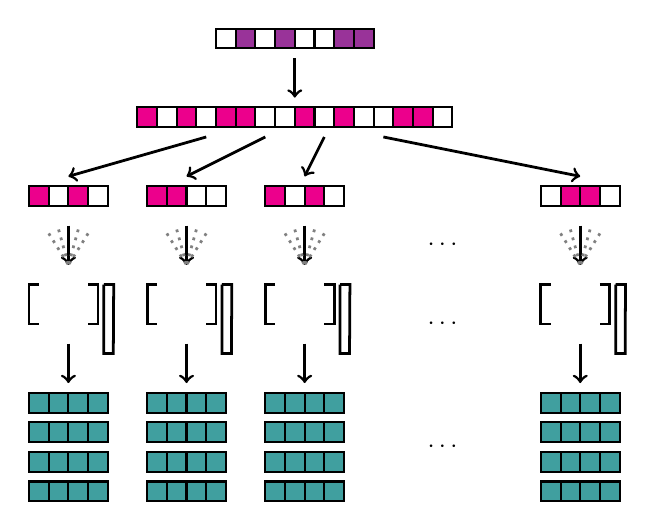
\begin{tikzpicture}
[font=\small, draw=black, line width=0.75pt,
sub0/.style={rectangle, draw, inner sep=0pt, minimum width=10mm, minimum height=2.5mm},
parity/.style={rectangle, draw, fill=teal!75, inner sep=0pt, minimum size=2.5mm},
bit0/.style={rectangle, draw, inner sep=0pt, minimum size=2.5mm},
bit1/.style={rectangle, draw, fill=violet!80, inner sep=0pt, minimum size=2.5mm},ebit0/.style={rectangle, draw, inner sep=0pt, minimum size=2.5mm},
ebit1/.style={rectangle, draw, fill=magenta, inner sep=0pt, minimum size=2.5mm}
]

\node[bit0] (info0) at (1.00,8.125) {};
\node[bit1] (info1) at (1.25,8.125) {};
\node[bit0] (info2) at (1.50,8.125) {};
\node[bit1] (info3) at (1.75,8.125) {};
\node[bit0] (info4) at (2.00,8.125) {};
\node[bit0] (info5) at (2.25,8.125) {};
\node[bit1] (info6) at (2.50,8.125) {};
\node[bit1] (info7) at (2.75,8.125) {};

\draw[->, line width=1pt]  (1.875,7.875) -- (1.875,7.375);

\node[ebit1] (bit0) at (0.00,7.125) {};
\node[ebit0] (bit1) at (0.25,7.125) {};
\node[ebit1] (bit2) at (0.50,7.125) {};
\node[ebit0] (bit3) at (0.75,7.125) {};
\node[ebit1] (bit4) at (1.00,7.125) {};
\node[ebit1] (bit5) at (1.25,7.125) {};
\node[ebit0] (bit6) at (1.50,7.125) {};
\node[ebit0] (bit7) at (1.75,7.125) {};
\node[ebit1] (bit8) at (2.00,7.125) {};
\node[ebit0] (bit9) at (2.25,7.125) {};
\node[ebit1] (bit10) at (2.50,7.125) {};
\node[ebit0] (bit11) at (2.75,7.125) {};
\node[ebit0] (bit12) at (3.00,7.125) {};
\node[ebit1] (bit13) at (3.25,7.125) {};
\node[ebit1] (bit14) at (3.50,7.125) {};
\node[ebit0] (bit15) at (3.75,7.125) {};

\draw[->, line width=1pt]  (0.75,6.875) -- (-1.00,6.375);
\draw[->, line width=1pt]  (1.50,6.875) -- (0.50,6.375);
\draw[->, line width=1pt]  (2.25,6.875) -- (2.00,6.375);
\draw[->, line width=1pt]  (3.00,6.875) -- (5.50,6.375);

\node[ebit1] (s00) at (-1.375,6.125) {};
\node[ebit0] (s01) at (-1.125,6.125) {};
\node[ebit1] (s02) at (-0.875,6.125) {};
\node[ebit0] (s02) at (-0.625,6.125) {};

\node[ebit1] (s03) at (0.125,6.125) {};
\node[ebit1] (s04) at (0.375,6.125) {};
\node[ebit0] (s05) at (0.625,6.125) {};
\node[ebit0] (s05) at (0.875,6.125) {};

\node[ebit1] (s06) at (1.625,6.125) {};
\node[ebit0] (s07) at (1.875,6.125) {};
\node[ebit1] (s08) at (2.125,6.125) {};
\node[ebit0] (s08) at (2.375,6.125) {};

\node[ebit0] (s09) at (5.125,6.125) {};
\node[ebit1] (s10) at (5.375,6.125) {};
\node[ebit1] (s11) at (5.625,6.125) {};
\node[ebit0] (s11) at (5.875,6.125) {};

\foreach \v in {-1.00,0.50,2.00,5.50} {
  \draw[->, line width=1pt]  (\v,4.25) -- (\v,3.75);
  \draw[->, line width=1pt]  (\v,5.75) -- (\v,5.25);
  \draw[dotted, line width=1pt, draw=gray]  (\v-0.25,5.65) -- (\v,5.25);
  \draw[dotted, line width=1pt, draw=gray]  (\v-0.125,5.7) -- (\v,5.25);
  \draw[dotted, line width=1pt, draw=gray]  (\v+0.125,5.7) -- (\v,5.25);
  \draw[dotted, line width=1pt, draw=gray]  (\v+0.25,5.65) -- (\v,5.25);
}

\node (dots1) at (3.75,5.5) {$\cdots$};

\foreach \v in {-1.00,0.50,2.00,5.50} {
  \draw[line width=1pt] (\v-0.375,5) -- (\v-0.5,5) -- (\v-0.5,4.5) -- (\v-0.375,4.5);
  \draw[line width=1pt] (\v+0.25,5) -- (\v+0.375,5) -- (\v+0.375,4.5) -- (\v+0.25,4.5);
  \draw[line width=1pt] (\v+0.45,5) -- (\v+0.45,4.125) -- (\v+0.57,4.125) -- (\v+0.575,5) -- (\v+0.45,5);
}

\node (dots2) at (3.75,4.5) {$\cdots$};
\node (dots3) at (3.75,2.9375) {$\cdots$};

\foreach \c in {3.50, 3.125, 2.75, 2.375} {
  \node[parity] (subcs00c\c) at (-1.375,\c) {};
  \node[parity] (subcs01c\c) at (-1.125,\c) {};
  \node[parity] (subcs02c\c) at (-0.875,\c) {};
  \node[parity] (subcs02c\c) at (-0.625,\c) {};

  \node[parity] (subcs03c\c) at (0.125,\c) {};
  \node[parity] (subcs04c\c) at (0.375,\c) {};
  \node[parity] (subcs05c\c) at (0.625,\c) {};
  \node[parity] (subcs05c\c) at (0.875,\c) {};

  \node[parity] (subcs06c\c) at (1.625,\c) {};
  \node[parity] (subcs07c\c) at (1.875,\c) {};
  \node[parity] (subcs08c\c) at (2.125,\c) {};
  \node[parity] (subcs08c\c) at (2.375,\c) {};

  \node[parity] (subcs09c\c) at (5.125,\c) {};
  \node[parity] (subcs10c\c) at (5.375,\c) {};
  \node[parity] (subcs11c\c) at (5.625,\c) {};
  \node[parity] (subcs11c\c) at (5.875,\c) {};
}

\end{tikzpicture}

\end{center}
\begin{itemize}
\item Data fragmentation and indexing
\item Outer encoding for disambiguation
\end{itemize}
\end{frame}

% % % % % % % % % % % % % % % % % % % %

\begin{frame}
\frametitle{CCS -- Approximate Message Passing}
\begin{center}
\begin{tikzpicture}
  \node[scope fading=south] (image) at (0,0) {\includegraphics[width=4in]{Figures-AMP/SparcsUMAC.png}};
\end{tikzpicture}
\end{center}
  \begin{itemize}
  \item Connection between CCS indexing and sparse regression codes
  \item Circumvent slotting under CCS and dispersion effects
  \item Introduce denoiser tailored to CCS
  \end{itemize}
\end{frame}

% % % % % % % % % % % % % % % % % % % %

\begin{frame}
\frametitle{CCS Revisited}
\begin{center}
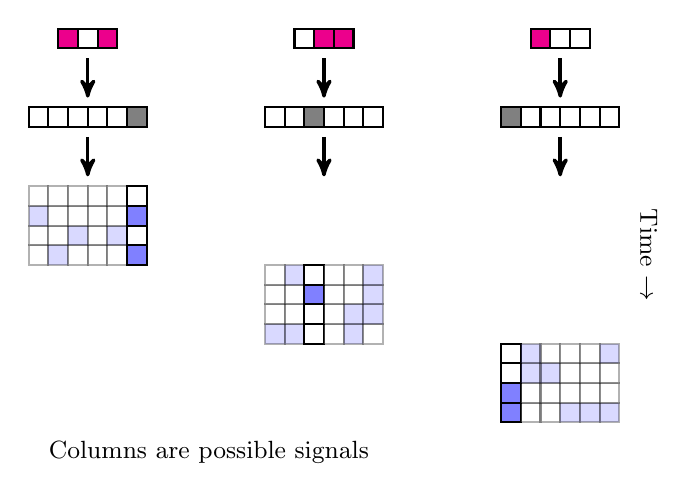
\begin{tikzpicture}
[font=\small, draw=black, line width=0.75pt, >=stealth',
ebit0/.style={rectangle, draw, inner sep=0pt, minimum size=2.5mm},
ebit1/.style={rectangle, draw, fill=magenta, inner sep=0pt, minimum size=2.5mm},
entry0/.style={rectangle, draw, opacity=0.3, fill=white, inner sep=0pt, minimum size=2.5mm},
entry1/.style={rectangle, draw, opacity=0.3, fill=blue!50, inner sep=0pt, minimum size=2.5mm},
entry00/.style={rectangle, draw, fill=white, inner sep=0pt, minimum size=2.5mm},
entry11/.style={rectangle, draw, fill=blue!50, inner sep=0pt, minimum size=2.5mm},
symbol0/.style={rectangle, draw, fill=white, inner sep=0pt, minimum size=2.5mm},
symbol1/.style={rectangle, draw, fill=gray, inner sep=0pt, minimum size=2.5mm}]

\node[entry11] (m2400) at (6.00,0) {};
\node[entry0] (m2500) at (6.25,0) {};
\node[entry0] (m2600) at (6.50,0) {};
\node[entry1] (m2700) at (6.75,0) {};
\node[entry1] (m2800) at (7.00,0) {};
\node[entry1] (m2900) at (7.25,0) {};

\node[entry11] (m2401) at (6.00,0.25) {};
\node[entry0] (m2501) at (6.25,0.25) {};
\node[entry0] (m2601) at (6.50,0.25) {};
\node[entry0] (m2701) at (6.75,0.25) {};
\node[entry0] (m2801) at (7.00,0.25) {};
\node[entry0] (m2901) at (7.25,0.25) {};

\node[entry00] (m2402) at (6.00,0.50) {};
\node[entry1] (m2502) at (6.25,0.50) {};
\node[entry1] (m2602) at (6.50,0.50) {};
\node[entry0] (m2702) at (6.75,0.50) {};
\node[entry0] (m2802) at (7.00,0.50) {};
\node[entry0] (m2902) at (7.25,0.50) {};

\node[entry00] (m2403) at (6.00,0.75) {};
\node[entry1] (m2503) at (6.25,0.75) {};
\node[entry0] (m2603) at (6.50,0.75) {};
\node[entry0] (m2703) at (6.75,0.75) {};
\node[entry0] (m2803) at (7.00,0.75) {};
\node[entry1] (m2903) at (7.25,0.75) {};

\node[entry1] (m1204) at (3.00,1.00) {};
\node[entry1] (m1304) at (3.25,1.00) {};
\node[entry00] (m1404) at (3.50,1.00) {};
\node[entry0] (m1504) at (3.75,1.00) {};
\node[entry1] (m1604) at (4.00,1.00) {};
\node[entry0] (m1704) at (4.25,1.00) {};

\node[entry0] (m1205) at (3.00,1.25) {};
\node[entry0] (m1305) at (3.25,1.25) {};
\node[entry00] (m1405) at (3.50,1.25) {};
\node[entry0] (m1505) at (3.75,1.25) {};
\node[entry1] (m1605) at (4.00,1.25) {};
\node[entry1] (m1705) at (4.25,1.25) {};

\node[entry0] (m1206) at (3.00,1.50) {};
\node[entry0] (m1306) at (3.25,1.50) {};
\node[entry11] (m1406) at (3.50,1.50) {};
\node[entry0] (m1506) at (3.75,1.50) {};
\node[entry0] (m1606) at (4.00,1.50) {};
\node[entry1] (m1706) at (4.25,1.50) {};

\node[entry0] (m1207) at (3.00,1.75) {};
\node[entry1] (m1307) at (3.25,1.75) {};
\node[entry00] (m1407) at (3.50,1.75) {};
\node[entry0] (m1507) at (3.75,1.75) {};
\node[entry0] (m1607) at (4.00,1.75) {};
\node[entry1] (m1707) at (4.25,1.75) {};

\node[entry0] (m0008) at (0.00,2.00) {};
\node[entry1] (m0108) at (0.25,2.00) {};
\node[entry0] (m0208) at (0.50,2.00) {};
\node[entry0] (m0308) at (0.75,2.00) {};
\node[entry0] (m0408) at (1.00,2.00) {};
\node[entry11] (m0508) at (1.25,2.00) {};

\node[entry0] (m0009) at (0.00,2.25) {};
\node[entry0] (m0109) at (0.25,2.25) {};
\node[entry1] (m0209) at (0.50,2.25) {};
\node[entry0] (m0309) at (0.75,2.25) {};
\node[entry1] (m0409) at (1.00,2.25) {};
\node[entry00] (m0509) at (1.25,2.25) {};

\node[entry1] (m0010) at (0.00,2.50) {};
\node[entry0] (m0110) at (0.25,2.50) {};
\node[entry0] (m0210) at (0.50,2.50) {};
\node[entry0] (m0310) at (0.75,2.50) {};
\node[entry0] (m0410) at (1.00,2.50) {};
\node[entry11] (m0510) at (1.25,2.50) {};

\node[entry0] (m0011) at (0.00,2.75) {};
\node[entry0] (m0111) at (0.25,2.75) {};
\node[entry0] (m0211) at (0.50,2.75) {};
\node[entry0] (m0311) at (0.75,2.75) {};
\node[entry0] (m0411) at (1.00,2.75) {};
\node[entry00] (m0511) at (1.25,2.75) {};

\draw[->, line width=1.25pt]  (0.625,3.50) -- (0.625,3.00);
\draw[->, line width=1.25pt]  (3.625,3.50) -- (3.625,3.00);
\draw[->, line width=1.25pt]  (6.625,3.50) -- (6.625,3.00);

\node[symbol0] (s00) at (0.00,3.75) {};
\node[symbol0] (s01) at (0.25,3.75) {};
\node[symbol0] (s02) at (0.50,3.75) {};
\node[symbol0] (s03) at (0.75,3.75) {};
\node[symbol0] (s04) at (1.00,3.75) {};
\node[symbol1] (s05) at (1.25,3.75) {};

\node[symbol0] (s12) at (3.00,3.75) {};
\node[symbol0] (s13) at (3.25,3.75) {};
\node[symbol1] (s14) at (3.50,3.75) {};
\node[symbol0] (s15) at (3.75,3.75) {};
\node[symbol0] (s16) at (4.00,3.75) {};
\node[symbol0] (s17) at (4.25,3.75) {};

\node[symbol1] (s24) at (6.00,3.75) {};
\node[symbol0] (s25) at (6.25,3.75) {};
\node[symbol0] (s26) at (6.50,3.75) {};
\node[symbol0] (s27) at (6.75,3.75) {};
\node[symbol0] (s28) at (7.00,3.75) {};
\node[symbol0] (s29) at (7.25,3.75) {};

\draw[->, line width=1.25pt]  (0.625,4.50) -- (0.625,4.00);
\draw[->, line width=1.25pt]  (3.625,4.50) -- (3.625,4.00);
\draw[->, line width=1.25pt]  (6.625,4.50) -- (6.625,4.00);

\node[ebit1] (info0) at (0.375,4.75) {};
\node[ebit0] (info1) at (0.625,4.75) {};
\node[ebit1] (info2) at (0.875,4.75) {};
\node[ebit0] (info3) at (3.375,4.75) {};
\node[ebit1] (info4) at (3.625,4.75) {};
\node[ebit1] (info5) at (3.875,4.75) {};
\node[ebit1] (info6) at (6.375,4.75) {};
\node[ebit0] (info7) at (6.625,4.75) {};
\node[ebit0] (info8) at (6.875,4.75) {};


\node [anchor = west] (signals) at (0.00,-0.50) {Columns are possible signals};
\node[rotate=-90] (time) at (7.75,2) {Time $\rightarrow$};
\end{tikzpicture}

\end{center}
\begin{itemize}
\item Bit sequence split into $L$ fragments
\item Each bit $+$ parity block converted to index in $[ 0, 2^{m/L}-1 ]$
\item Stack sub-codewords into $(n/L) \times 2^{m/L}$ sensing matrices
\end{itemize}
\end{frame}

% % % % % % % % % % % % % % % % % % % %

\begin{frame}
\frametitle{Coded Compressed Sensing -- Unified View}
% % % % %
\begin{center}
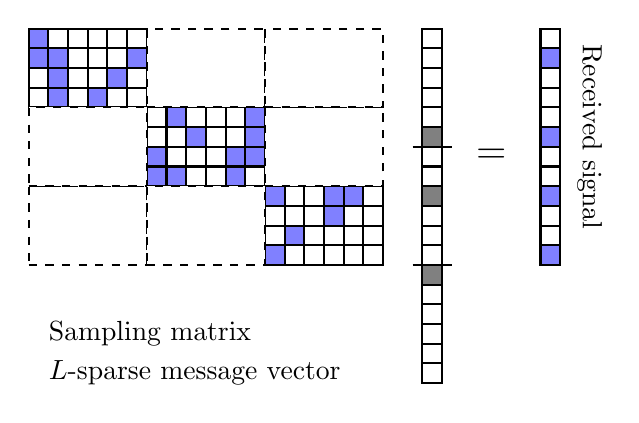
\begin{tikzpicture}
[draw=black, line width=0.75pt,
block/.style={rectangle, draw, fill=white, inner sep=0pt, minimum width=15mm,minimum height=10mm},
entry1/.style={rectangle, draw, fill=blue!50, inner sep=0pt, minimum size=2.5mm},
entry0/.style={rectangle, draw, fill=white, inner sep=0pt, minimum size=2.5mm},
symbol0/.style={rectangle, draw, fill=white, inner sep=0pt, minimum size=2.5mm},
symbol1/.style={rectangle, draw, fill=gray, inner sep=0pt, minimum size=2.5mm},
signal0/.style={rectangle, draw, fill=white, inner sep=0pt, minimum size=2.5mm},
signal1/.style={rectangle, draw, fill=blue!50, inner sep=0pt, minimum size=2.5mm}
]

\node[entry1] (m1800) at (4.50,0) {};
\node[entry0] (m1900) at (4.75,0) {};
\node[entry0] (m2000) at (5.00,0) {};
\node[entry0] (m2100) at (5.25,0) {};
\node[entry0] (m2200) at (5.50,0) {};
\node[entry0] (m2300) at (5.75,0) {};

\node[entry0] (m1801) at (4.50,0.25) {};
\node[entry1] (m1901) at (4.75,0.25) {};
\node[entry0] (m2001) at (5.00,0.25) {};
\node[entry0] (m2101) at (5.25,0.25) {};
\node[entry0] (m2201) at (5.50,0.25) {};
\node[entry0] (m2301) at (5.75,0.25) {};

\node[entry0] (m1802) at (4.50,0.50) {};
\node[entry0] (m1902) at (4.75,0.50) {};
\node[entry0] (m2002) at (5.00,0.50) {};
\node[entry1] (m2102) at (5.25,0.50) {};
\node[entry0] (m2202) at (5.50,0.50) {};
\node[entry0] (m2302) at (5.75,0.50) {};

\node[entry1] (m1803) at (4.50,0.75) {};
\node[entry0] (m1903) at (4.75,0.75) {};
\node[entry0] (m2003) at (5.00,0.75) {};
\node[entry1] (m2103) at (5.25,0.75) {};
\node[entry1] (m2203) at (5.50,0.75) {};
\node[entry0] (m2303) at (5.75,0.75) {};

\node[entry1] (m1204) at (3.00,1.00) {};
\node[entry1] (m1304) at (3.25,1.00) {};
\node[entry0] (m1404) at (3.50,1.00) {};
\node[entry0] (m1504) at (3.75,1.00) {};
\node[entry1] (m1604) at (4.00,1.00) {};
\node[entry0] (m1704) at (4.25,1.00) {};

\node[entry1] (m1205) at (3.00,1.25) {};
\node[entry0] (m1305) at (3.25,1.25) {};
\node[entry0] (m1405) at (3.50,1.25) {};
\node[entry0] (m1505) at (3.75,1.25) {};
\node[entry1] (m1605) at (4.00,1.25) {};
\node[entry1] (m1705) at (4.25,1.25) {};

\node[entry0] (m1206) at (3.00,1.50) {};
\node[entry0] (m1306) at (3.25,1.50) {};
\node[entry1] (m1406) at (3.50,1.50) {};
\node[entry0] (m1506) at (3.75,1.50) {};
\node[entry0] (m1606) at (4.00,1.50) {};
\node[entry1] (m1706) at (4.25,1.50) {};

\node[entry0] (m1207) at (3.00,1.75) {};
\node[entry1] (m1307) at (3.25,1.75) {};
\node[entry0] (m1407) at (3.50,1.75) {};
\node[entry0] (m1507) at (3.75,1.75) {};
\node[entry0] (m1607) at (4.00,1.75) {};
\node[entry1] (m1707) at (4.25,1.75) {};

\node[entry0] (m0608) at (1.50,2.00) {};
\node[entry1] (m0708) at (1.75,2.00) {};
\node[entry0] (m0808) at (2.00,2.00) {};
\node[entry1] (m0908) at (2.25,2.00) {};
\node[entry0] (m1008) at (2.50,2.00) {};
\node[entry0] (m1108) at (2.75,2.00) {};

\node[entry0] (m0609) at (1.50,2.25) {};
\node[entry1] (m0709) at (1.75,2.25) {};
\node[entry0] (m0809) at (2.00,2.25) {};
\node[entry0] (m0909) at (2.25,2.25) {};
\node[entry1] (m1009) at (2.50,2.25) {};
\node[entry0] (m1109) at (2.75,2.25) {};

\node[entry1] (m0610) at (1.50,2.50) {};
\node[entry1] (m0710) at (1.75,2.50) {};
\node[entry0] (m0810) at (2.00,2.50) {};
\node[entry0] (m0910) at (2.25,2.50) {};
\node[entry0] (m1010) at (2.50,2.50) {};
\node[entry1] (m1110) at (2.75,2.50) {};

\node[entry1] (m0611) at (1.50,2.75) {};
\node[entry0] (m0711) at (1.75,2.75) {};
\node[entry0] (m0811) at (2.00,2.75) {};
\node[entry0] (m0911) at (2.25,2.75) {};
\node[entry0] (m1011) at (2.50,2.75) {};
\node[entry0] (m1111) at (2.75,2.75) {};

\node[block,dashed] at (2.125,0.375) {};
\node[block,dashed] at (2.125,1.375) {};
\node[block,dashed] at (3.625,0.375) {};
\node[block,dashed] at (3.625,2.375) {};
\node[block,dashed] at (5.125,1.375) {};
\node[block,dashed] at (5.125,2.375) {};

\node[symbol0] (s07) at (6.5,-1.50) {};
\node[symbol0] (s08) at (6.5,-1.25) {};
\node[symbol0] (s09) at (6.5,-1.00) {};
\node[symbol0] (s10) at (6.5,-0.75) {};
\node[symbol0] (s11) at (6.5,-0.50) {};
\node[symbol1] (s12) at (6.5,-0.25) {};
\draw (6.25,-0.125) -- (6.75,-0.125);
\node[symbol0] (s13) at (6.5,0) {};
\node[symbol0] (s14) at (6.5,0.25) {};
\node[symbol0] (s15) at (6.5,0.50) {};
\node[symbol1] (s16) at (6.5,0.75) {};
\node[symbol0] (s17) at (6.5,1.00) {};
\node[symbol0] (s18) at (6.5,1.25) {};
\draw (6.25,1.375) -- (6.75,1.375);
\node[symbol1] (s19) at (6.5,1.50) {};
\node[symbol0] (s20) at (6.5,1.75) {};
\node[symbol0] (s21) at (6.5,2.00) {};
\node[symbol0] (s22) at (6.5,2.25) {};
\node[symbol0] (s23) at (6.5,2.50) {};
\node[symbol0] (s24) at (6.5,2.75) {};

\node (equal) at (7.25,1.25) {\Large =};

\node[signal1] (y00) at (8,0) {};
\node[signal0] (y01) at (8,0.25) {};
\node[signal0] (y02) at (8,0.50) {};
\node[signal1] (y03) at (8,0.75) {};
\node[signal0] (y04) at (8,1.00) {};
\node[signal0] (y05) at (8,1.25) {};
\node[signal1] (y06) at (8,1.50) {};
\node[signal0] (y07) at (8,1.75) {};
\node[signal0] (y08) at (8,2.00) {};
\node[signal0] (y09) at (8,2.25) {};
\node[signal1] (y10) at (8,2.50) {};
\node[signal0] (y11) at (8,2.75) {};

\node[anchor=west] (samplingmatrix) at (1.5,-1) {Sampling matrix};
\node[anchor=west] (vector) at (1.5,-1.5) {$L$-sparse message vector};
\node[rotate=-90] (receivedsignal) at (8.5,1.5) {Received signal};
\end{tikzpicture}

\end{center}
\begin{itemize}
\item Slots produce block diagonal (unified) matrix
\item Message is one-sparse per section
\item Width of $\Am$ is smaller: $L 2^{m/L}$ instead of $2^m$
\end{itemize}
\end{frame}

% % % % % % % % % % % % % % % % % % % %

\begin{frame}
\frametitle{CCS -- Full Sensing Matrix}
% % % % %
\begin{center}
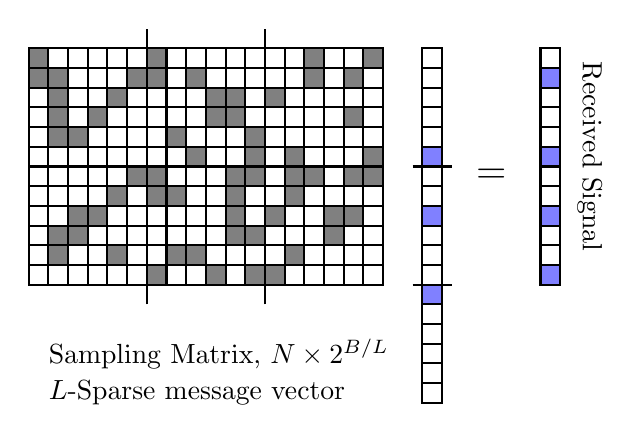
\begin{tikzpicture}
[draw=black, line width=0.75pt,
entry0/.style={rectangle, draw, fill=white, inner sep=0pt, minimum size=2.5mm},
entry1/.style={rectangle, draw, fill=gray, inner sep=0pt, minimum size=2.5mm},
symbol0/.style={rectangle, draw, fill=white, inner sep=0pt, minimum size=2.5mm},
symbol1/.style={rectangle, draw, fill=blue!50, inner sep=0pt, minimum size=2.5mm}]

\node[entry0] (m0600) at (1.50,0) {};
\node[entry0] (m0700) at (1.75,0) {};
\node[entry0] (m0800) at (2.00,0) {};
\node[entry0] (m0900) at (2.25,0) {};
\node[entry0] (m1000) at (2.50,0) {};
\node[entry0] (m1100) at (2.75,0) {};
\node[entry1] (m1200) at (3.00,0) {};
\node[entry0] (m1300) at (3.25,0) {};
\node[entry0] (m1400) at (3.50,0) {};
\node[entry1] (m1500) at (3.75,0) {};
\node[entry0] (m1600) at (4.00,0) {};
\node[entry1] (m1700) at (4.25,0) {};
\node[entry1] (m1800) at (4.50,0) {};
\node[entry0] (m1900) at (4.75,0) {};
\node[entry0] (m2000) at (5.00,0) {};
\node[entry0] (m2100) at (5.25,0) {};
\node[entry0] (m2200) at (5.50,0) {};
\node[entry0] (m2300) at (5.75,0) {};

\node[entry0] (m0601) at (1.50,0.25) {};
\node[entry1] (m0701) at (1.75,0.25) {};
\node[entry0] (m0801) at (2.00,0.25) {};
\node[entry0] (m0901) at (2.25,0.25) {};
\node[entry1] (m1001) at (2.50,0.25) {};
\node[entry0] (m1101) at (2.75,0.25) {};
\node[entry0] (m1201) at (3.00,0.25) {};
\node[entry1] (m1301) at (3.25,0.25) {};
\node[entry1] (m1401) at (3.50,0.25) {};
\node[entry0] (m1501) at (3.75,0.25) {};
\node[entry0] (m1601) at (4.00,0.25) {};
\node[entry0] (m1701) at (4.25,0.25) {};
\node[entry0] (m1801) at (4.50,0.25) {};
\node[entry1] (m1901) at (4.75,0.25) {};
\node[entry0] (m2001) at (5.00,0.25) {};
\node[entry0] (m2101) at (5.25,0.25) {};
\node[entry0] (m2201) at (5.50,0.25) {};
\node[entry0] (m2301) at (5.75,0.25) {};

\node[entry0] (m0602) at (1.50,0.50) {};
\node[entry1] (m0702) at (1.75,0.50) {};
\node[entry1] (m0802) at (2.00,0.50) {};
\node[entry0] (m0902) at (2.25,0.50) {};
\node[entry0] (m1002) at (2.50,0.50) {};
\node[entry0] (m1102) at (2.75,0.50) {};
\node[entry0] (m1202) at (3.00,0.50) {};
\node[entry0] (m1302) at (3.25,0.50) {};
\node[entry0] (m1402) at (3.50,0.50) {};
\node[entry0] (m1502) at (3.75,0.50) {};
\node[entry1] (m1602) at (4.00,0.50) {};
\node[entry1] (m1702) at (4.25,0.50) {};
\node[entry0] (m1802) at (4.50,0.50) {};
\node[entry0] (m1902) at (4.75,0.50) {};
\node[entry0] (m2002) at (5.00,0.50) {};
\node[entry1] (m2102) at (5.25,0.50) {};
\node[entry0] (m2202) at (5.50,0.50) {};
\node[entry0] (m2302) at (5.75,0.50) {};

\node[entry0] (m0603) at (1.50,0.75) {};
\node[entry0] (m0703) at (1.75,0.75) {};
\node[entry1] (m0803) at (2.00,0.75) {};
\node[entry1] (m0903) at (2.25,0.75) {};
\node[entry0] (m1003) at (2.50,0.75) {};
\node[entry0] (m1103) at (2.75,0.75) {};
\node[entry0] (m1203) at (3.00,0.75) {};
\node[entry0] (m1303) at (3.25,0.75) {};
\node[entry0] (m1403) at (3.50,0.75) {};
\node[entry0] (m1503) at (3.75,0.75) {};
\node[entry1] (m1603) at (4.00,0.75) {};
\node[entry0] (m1703) at (4.25,0.75) {};
\node[entry1] (m1803) at (4.50,0.75) {};
\node[entry0] (m1903) at (4.75,0.75) {};
\node[entry0] (m2003) at (5.00,0.75) {};
\node[entry1] (m2103) at (5.25,0.75) {};
\node[entry1] (m2203) at (5.50,0.75) {};
\node[entry0] (m2303) at (5.75,0.75) {};

\node[entry0] (m0604) at (1.50,1.00) {};
\node[entry0] (m0704) at (1.75,1.00) {};
\node[entry0] (m0804) at (2.00,1.00) {};
\node[entry0] (m0904) at (2.25,1.00) {};
\node[entry1] (m1004) at (2.50,1.00) {};
\node[entry0] (m1104) at (2.75,1.00) {};
\node[entry1] (m1204) at (3.00,1.00) {};
\node[entry1] (m1304) at (3.25,1.00) {};
\node[entry0] (m1404) at (3.50,1.00) {};
\node[entry0] (m1504) at (3.75,1.00) {};
\node[entry1] (m1604) at (4.00,1.00) {};
\node[entry0] (m1704) at (4.25,1.00) {};
\node[entry0] (m1804) at (4.50,1.00) {};
\node[entry1] (m1904) at (4.75,1.00) {};
\node[entry0] (m2004) at (5.00,1.00) {};
\node[entry0] (m2104) at (5.25,1.00) {};
\node[entry0] (m2204) at (5.50,1.00) {};
\node[entry0] (m2304) at (5.75,1.00) {};

\node[entry0] (m0605) at (1.50,1.25) {};
\node[entry0] (m0705) at (1.75,1.25) {};
\node[entry0] (m0805) at (2.00,1.25) {};
\node[entry0] (m0905) at (2.25,1.25) {};
\node[entry0] (m1005) at (2.50,1.25) {};
\node[entry1] (m1105) at (2.75,1.25) {};
\node[entry1] (m1205) at (3.00,1.25) {};
\node[entry0] (m1305) at (3.25,1.25) {};
\node[entry0] (m1405) at (3.50,1.25) {};
\node[entry0] (m1505) at (3.75,1.25) {};
\node[entry1] (m1605) at (4.00,1.25) {};
\node[entry1] (m1705) at (4.25,1.25) {};
\node[entry0] (m1805) at (4.50,1.25) {};
\node[entry1] (m1905) at (4.75,1.25) {};
\node[entry1] (m2005) at (5.00,1.25) {};
\node[entry0] (m2105) at (5.25,1.25) {};
\node[entry1] (m2205) at (5.50,1.25) {};
\node[entry1] (m2305) at (5.75,1.25) {};

\node[entry0] (m0606) at (1.50,1.50) {};
\node[entry0] (m0706) at (1.75,1.50) {};
\node[entry0] (m0806) at (2.00,1.50) {};
\node[entry0] (m0906) at (2.25,1.50) {};
\node[entry0] (m1006) at (2.50,1.50) {};
\node[entry0] (m1106) at (2.75,1.50) {};
\node[entry0] (m1206) at (3.00,1.50) {};
\node[entry0] (m1306) at (3.25,1.50) {};
\node[entry1] (m1406) at (3.50,1.50) {};
\node[entry0] (m1506) at (3.75,1.50) {};
\node[entry0] (m1606) at (4.00,1.50) {};
\node[entry1] (m1706) at (4.25,1.50) {};
\node[entry0] (m1806) at (4.50,1.50) {};
\node[entry1] (m1906) at (4.75,1.50) {};
\node[entry0] (m2006) at (5.00,1.50) {};
\node[entry0] (m2106) at (5.25,1.50) {};
\node[entry0] (m2206) at (5.50,1.50) {};
\node[entry1] (m2306) at (5.75,1.50) {};

\node[entry0] (m0607) at (1.50,1.75) {};
\node[entry1] (m0707) at (1.75,1.75) {};
\node[entry1] (m0807) at (2.00,1.75) {};
\node[entry0] (m0907) at (2.25,1.75) {};
\node[entry0] (m1007) at (2.50,1.75) {};
\node[entry0] (m1107) at (2.75,1.75) {};
\node[entry0] (m1207) at (3.00,1.75) {};
\node[entry1] (m1307) at (3.25,1.75) {};
\node[entry0] (m1407) at (3.50,1.75) {};
\node[entry0] (m1507) at (3.75,1.75) {};
\node[entry0] (m1607) at (4.00,1.75) {};
\node[entry1] (m1707) at (4.25,1.75) {};
\node[entry0] (m1807) at (4.50,1.75) {};
\node[entry0] (m1907) at (4.75,1.75) {};
\node[entry0] (m2007) at (5.00,1.75) {};
\node[entry0] (m2107) at (5.25,1.75) {};
\node[entry0] (m2207) at (5.50,1.75) {};
\node[entry0] (m2307) at (5.75,1.75) {};

\node[entry0] (m0608) at (1.50,2.00) {};
\node[entry1] (m0708) at (1.75,2.00) {};
\node[entry0] (m0808) at (2.00,2.00) {};
\node[entry1] (m0908) at (2.25,2.00) {};
\node[entry0] (m1008) at (2.50,2.00) {};
\node[entry0] (m1108) at (2.75,2.00) {};
\node[entry0] (m1208) at (3.00,2.00) {};
\node[entry0] (m1308) at (3.25,2.00) {};
\node[entry0] (m1408) at (3.50,2.00) {};
\node[entry1] (m1508) at (3.75,2.00) {};
\node[entry1] (m1608) at (4.00,2.00) {};
\node[entry0] (m1708) at (4.25,2.00) {};
\node[entry0] (m1808) at (4.50,2.00) {};
\node[entry0] (m1908) at (4.75,2.00) {};
\node[entry0] (m2008) at (5.00,2.00) {};
\node[entry0] (m2108) at (5.25,2.00) {};
\node[entry1] (m2208) at (5.50,2.00) {};
\node[entry0] (m2308) at (5.75,2.00) {};

\node[entry0] (m0609) at (1.50,2.25) {};
\node[entry1] (m0709) at (1.75,2.25) {};
\node[entry0] (m0809) at (2.00,2.25) {};
\node[entry0] (m0909) at (2.25,2.25) {};
\node[entry1] (m1009) at (2.50,2.25) {};
\node[entry0] (m1109) at (2.75,2.25) {};
\node[entry0] (m1209) at (3.00,2.25) {};
\node[entry0] (m1309) at (3.25,2.25) {};
\node[entry0] (m1409) at (3.50,2.25) {};
\node[entry1] (m1509) at (3.75,2.25) {};
\node[entry1] (m1609) at (4.00,2.25) {};
\node[entry0] (m1709) at (4.25,2.25) {};
\node[entry1] (m1809) at (4.50,2.25) {};
\node[entry0] (m1909) at (4.75,2.25) {};
\node[entry0] (m2009) at (5.00,2.25) {};
\node[entry0] (m2109) at (5.25,2.25) {};
\node[entry0] (m2209) at (5.50,2.25) {};
\node[entry0] (m2309) at (5.75,2.25) {};

\node[entry1] (m0610) at (1.50,2.50) {};
\node[entry1] (m0710) at (1.75,2.50) {};
\node[entry0] (m0810) at (2.00,2.50) {};
\node[entry0] (m0910) at (2.25,2.50) {};
\node[entry0] (m1010) at (2.50,2.50) {};
\node[entry1] (m1110) at (2.75,2.50) {};
\node[entry1] (m1210) at (3.00,2.50) {};
\node[entry0] (m1310) at (3.25,2.50) {};
\node[entry1] (m1410) at (3.50,2.50) {};
\node[entry0] (m1510) at (3.75,2.50) {};
\node[entry0] (m1610) at (4.00,2.50) {};
\node[entry0] (m1710) at (4.25,2.50) {};
\node[entry0] (m1810) at (4.50,2.50) {};
\node[entry0] (m1910) at (4.75,2.50) {};
\node[entry1] (m2010) at (5.00,2.50) {};
\node[entry0] (m2110) at (5.25,2.50) {};
\node[entry1] (m2210) at (5.50,2.50) {};
\node[entry0] (m2310) at (5.75,2.50) {};

\node[entry1] (m0611) at (1.50,2.75) {};
\node[entry0] (m0711) at (1.75,2.75) {};
\node[entry0] (m0811) at (2.00,2.75) {};
\node[entry0] (m0911) at (2.25,2.75) {};
\node[entry0] (m1011) at (2.50,2.75) {};
\node[entry0] (m1111) at (2.75,2.75) {};
\node[entry1] (m1211) at (3.00,2.75) {};
\node[entry0] (m1311) at (3.25,2.75) {};
\node[entry0] (m1411) at (3.50,2.75) {};
\node[entry0] (m1511) at (3.75,2.75) {};
\node[entry0] (m1611) at (4.00,2.75) {};
\node[entry0] (m1711) at (4.25,2.75) {};
\node[entry0] (m1811) at (4.50,2.75) {};
\node[entry0] (m1911) at (4.75,2.75) {};
\node[entry1] (m2011) at (5.00,2.75) {};
\node[entry0] (m2111) at (5.25,2.75) {};
\node[entry0] (m2211) at (5.50,2.75) {};
\node[entry1] (m2311) at (5.75,2.75) {};

\draw (2.875,-0.375) -- (2.875,3.125);
\draw (4.375,-0.375) -- (4.375,3.125);

\node[symbol0] (s07) at (6.5,-1.50) {};
\node[symbol0] (s08) at (6.5,-1.25) {};
\node[symbol0] (s09) at (6.5,-1.00) {};
\node[symbol0] (s10) at (6.5,-0.75) {};
\node[symbol0] (s11) at (6.5,-0.50) {};
\node[symbol1] (s12) at (6.5,-0.25) {};
\draw (6.25,-0.125) -- (6.75,-0.125);
\node[symbol0] (s13) at (6.5,0) {};
\node[symbol0] (s14) at (6.5,0.25) {};
\node[symbol0] (s15) at (6.5,0.50) {};
\node[symbol1] (s16) at (6.5,0.75) {};
\node[symbol0] (s17) at (6.5,1.00) {};
\node[symbol0] (s18) at (6.5,1.25) {};
\draw (6.25,1.375) -- (6.75,1.375);
\node[symbol1] (s19) at (6.5,1.50) {};
\node[symbol0] (s20) at (6.5,1.75) {};
\node[symbol0] (s21) at (6.5,2.00) {};
\node[symbol0] (s22) at (6.5,2.25) {};
\node[symbol0] (s23) at (6.5,2.50) {};
\node[symbol0] (s24) at (6.5,2.75) {};

\node (equal) at (7.25,1.25) {\Large =};

\node[symbol1] (y00) at (8,0) {};
\node[symbol0] (y01) at (8,0.25) {};
\node[symbol0] (y02) at (8,0.50) {};
\node[symbol1] (y03) at (8,0.75) {};
\node[symbol0] (y04) at (8,1.00) {};
\node[symbol0] (y05) at (8,1.25) {};
\node[symbol1] (y06) at (8,1.50) {};
\node[symbol0] (y07) at (8,1.75) {};
\node[symbol0] (y08) at (8,2.00) {};
\node[symbol0] (y09) at (8,2.25) {};
\node[symbol1] (y10) at (8,2.50) {};
\node[symbol0] (y11) at (8,2.75) {};

\node[anchor=west] (samplingmatrix) at (1.5,-1) {Sampling Matrix, $N \times 2^{{B}/{L}}$};
\node[anchor=west] (vector) at (1.5,-1.5) {$L$-Sparse message vector};
\node[rotate=-90] (receivedsignal) at (8.5,1.5) {Received Signal};
\end{tikzpicture}

\end{center}
\begin{itemize}
\item Complexity reduction due to narrower $\Am$
\item Use full sensing matrix $\Am$
\item Decode inner code with low-complexity AMP
\end{itemize}
%\myfootnote{\tiny
%A. Fengler, P. Jung, and G. Caire.
%\emph{SPARCs and AMP for Unsourced Random Access}.
%ISIT 2019}
\end{frame}

% % % % % % % % % % % % % % % % % % % %

\begin{frame}
\frametitle{CCS -- Approximate Message Passing}
% % % % %
\begin{block}{Governing Equations}
\begin{itemize}
\item AMP algorithm iterates through
\begin{align*}
\zv^{(t)} &= \yv - \Am \Dm \etav_t \big( \rv^{(t)} \big)
+ \underbrace{\frac{\zv^{(t-1)}}{n} \operatorname{div} \mathbf{D} \etav_t \big( \rv^{(t)} \big)}_{\text{Onsager correction}} \\
\rv^{(t+1)} &= \Am^{\transpose} \zv^{(t)} + \Dm
\underbrace{\etav_t \big( \rv^{(t)} \big)}_{\text{Denoiser}}
\end{align*}
\textcolor{gray}{Initial conditions $\zv^{(0)} = \zerov$ and $\etav_0 \left( \rv^{(0)} \right) = \zerov$}
\item Application falls within framework for non-separable functions
\end{itemize}
\end{block}
% % % % %
\vfill
% % % % %
\begin{exampleblock}{Task}
\begin{itemize}
\item Define denoiser and compute Onsager correction term
\end{itemize}
\end{exampleblock}
\end{frame}

% % % % % % % % % % % % % % % % % % % %

\begin{frame}
\frametitle{Marginal Posterior Mean Estimate (PME)}
% % % % %
\begin{block}{Proposed Denoiser (Fengler, Jung, and Caire)}
\begin{itemize}
\item State estimate based on Gaussian model
\begin{equation*}
\begin{split}
\hat{s}^{\mathrm{OR}} & \left( q, r, \tau \right)
= \mathbb{E} \left[ s \middle| \sqrt{P_{\ell}} s + \tau \zeta = r \right] \\
%&= \frac{0 \cdot \Pr (s = 0) f \left( \frac{r}{\tau} \right) + 1 \cdot \Pr (s = 1) f \left( \frac{r - d_{\ell}}{\tau} \right)}{\Pr (s = 0) f \left( \frac{r}{\tau} \right) + \Pr (s = 1) f \left( \frac{r - d_{\ell}}{\tau} \right)} \\
&= \frac{q \exp \left( - \frac{ \left( r - \sqrt{P_{\ell}} \right)^2}{2 \tau^2} \right)}
{(1-q) \exp \left( -\frac{r^2}{2 \tau^2} \right)
+ q \exp \left( - \frac{ \left( r - \sqrt{P_{\ell}} \right)^2}{2 \tau^2} \right)}
\end{split}
\end{equation*}
with (essentially) uninformative prior $q = K/m$ fixed
\item $\etav_t \left( \mathbf{r}^{(t)} \right)$ is aggregate of PME values
\item $\tau_t$ is obtained from state evolution or $\tau_t^2 = {\| \mathbf{z}^{(t)} \|^2}/{n}$
\end{itemize}
\end{block}
\end{frame}

% % % % % % % % % % % % % % % % % % % %

\begin{frame}
\frametitle{Performance of CCS-AMP versus Previous Schemes}
% % % % %
\begin{center}
\input{Figures-AMP/CCS-AMP-Performance1}
\end{center}
\end{frame}

% % % % % % % % % % % % % % % % % % % %

\begin{frame}
\frametitle{Incorporating Lessons from Enhanced CCS}
% % % % %
\begin{itemize}
\item Integrate outer code structure into inner decoding
\end{itemize}
\begin{center}
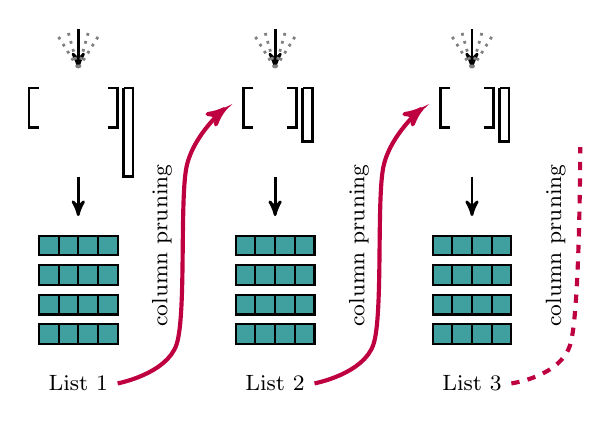
\begin{tikzpicture}
[font=\footnotesize, draw=black, line width=0.75pt,>=stealth',
sub0/.style={rectangle, draw, inner sep=0pt, minimum width=10mm, minimum height=2.5mm},
parity/.style={rectangle, draw, fill=teal!75, inner sep=0pt, minimum size=2.5mm}]

%\node (cs1) at (0.00,6.125) {Slot~1};
%\node (cs2) at (2.50,6.125) {Slot~2};
%\node (cs3) at (5.00,6.125) {Slot~3};

\foreach \v in {0.00,2.50,5.00} {
  \draw[->, line width=1pt]  (\v,3.875) -- (\v,3.375);
  \draw[->, line width=1pt]  (\v,5.75) -- (\v,5.25);
  \draw[dotted, line width=1pt, draw=gray]  (\v-0.25,5.65) -- (\v,5.25);
  \draw[dotted, line width=1pt, draw=gray]  (\v-0.125,5.7) -- (\v,5.25);
  \draw[dotted, line width=1pt, draw=gray]  (\v+0.125,5.7) -- (\v,5.25);
  \draw[dotted, line width=1pt, draw=gray]  (\v+0.25,5.65) -- (\v,5.25);
}

\foreach \v in {0.00} {
  \draw[line width=1pt] (\v-0.5,5) -- (\v-0.625,5) -- (\v-0.625,4.5) -- (\v-0.5,4.5);
  \draw[line width=1pt] (\v+0.375,5) -- (\v+0.5,5) -- (\v+0.5,4.5) -- (\v+0.375,4.5);
  \draw[line width=1pt] (\v+0.575,5) -- (\v+0.575,3.875) -- (\v+0.695,3.875) -- (\v+0.695,5) -- (\v+0.575,5);
}

\foreach \v in {2.50,5.00} {
  \draw[line width=1pt] (\v-0.275,5) -- (\v-0.4,5) -- (\v-0.4,4.5) -- (\v-0.275,4.5);
  \draw[line width=1pt] (\v+0.15,5) -- (\v+0.275,5) -- (\v+0.275,4.5) -- (\v+0.15,4.5);
  \draw[line width=1pt] (\v+0.35,5) -- (\v+0.35,4.325) -- (\v+0.47,4.325) -- (\v+0.47,5) -- (\v+0.35,5);
}

\foreach \p/\c in {3.00/1, 2.625/2, 2.25/3, 1.875/4} {
  \node[parity] (subcs00c\c) at (-0.375,\p) {};
  \node[parity] (subcs01c\c) at (-0.125,\p) {};
  \node[parity] (subcs02c\c) at (0.125,\p) {};
  \node[parity] (subcs02c\c) at (0.375,\p) {};

  \node[parity] (subcs03c\c) at (2.125,\p) {};
  \node[parity] (subcs04c\c) at (2.375,\p) {};
  \node[parity] (subcs05c\c) at (2.625,\p) {};
  \node[parity] (subcs05c\c) at (2.875,\p) {};

  \node[parity] (subcs06c\c) at (4.625,\p) {};
  \node[parity] (subcs07c\c) at (4.875,\p) {};
  \node[parity] (subcs08c\c) at (5.125,\p) {};
  \node[parity] (subcs08c\c) at (5.375,\p) {};
}



\node (list1) at (0.00,1.25) {List~1};
\node (list2) at (2.50,1.25) {List~2};
\node (list3) at (5.00,1.25) {List~3};

\draw [line width=1.5pt,color=purple,->] plot[smooth, tension=.5] coordinates {(0.5,1.25) (1.25,1.75) (1.375,4) (1.875,4.75)};
\draw [line width=1.5pt,color=purple,->] plot[smooth, tension=.5] coordinates {(3.0,1.25) (3.75,1.75) (3.875,4) (4.375,4.75)};
\draw [line width=1.5pt,color=purple,dashed] plot[smooth, tension=.5] coordinates {(5.5,1.25) (6.25,1.75) (6.375,4.25)};

\node[rotate=90] (prune1) at (1.0625,3) {column pruning};
\node[rotate=90] (prune2) at (3.5625,3) {column pruning};
\node[rotate=90] (prune3) at (6.0625,3) {column pruning};
\end{tikzpicture}

\end{center}
\begin{alertblock}{Challenges}
\begin{itemize}
\item CCS-AMP inner decoding is not a sequence of hard decisions
\item List size for CCS-AMP is effective length of index vector
\end{itemize}
\end{alertblock}
\myfootnote{\tiny
V.~K. Amalladinne, A.~K. Pradhan, C. Rush, J.-F. Chamberland, K.~R. Narayanan.
\emph{On approximate message passing for unsourced access with coded compressed sensing.}
ISIT 2020}

\end{frame}

% % % % % % % % % % % % % % % % % % % %

\begin{frame}
\frametitle{Redesigning Outer Code}
% % % % %
\begin{block}{Properties of Original Outer Code}
\begin{itemize}
\item Aimed at stitching message fragments together
\item Works on short lists of $K$ fragments
\item Parities allocated to control growth and complexity
\end{itemize}
\end{block}
\begin{center}
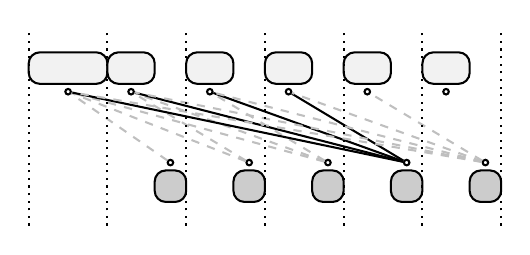
\begin{tikzpicture}[
  font=\footnotesize, >=stealth', line width=0.75pt,
  infobits0/.style={rectangle, minimum height=4mm, minimum width=10mm, draw=black, fill=gray!10, rounded corners},
  infobits/.style={rectangle, minimum height=4mm, minimum width=6mm, draw=black, fill=gray!10, rounded corners},
  paritybits/.style={rectangle, minimum height=4mm, minimum width=4mm, draw=black, fill=gray!40, rounded corners},
  dot/.style={circle, minimum width=2pt, draw=black, inner sep=0pt}
]

\node[infobits0] (vb0) at (0,1.5) {};
\node[infobits] (vb1) at (0.8,1.5) {};
\node[paritybits] (vp1) at (1.3,0) {};
\node[infobits] (vb2) at (1.8,1.5) {};
\node[paritybits] (vp2) at (2.3,0) {};
\node[infobits] (vb3) at (2.8,1.5) {};
\node[paritybits] (vp3) at (3.3,0) {};
\node[infobits] (vb4) at (3.8,1.5) {};
\node[paritybits] (vp4) at (4.3,0) {};
\node[infobits] (vb5) at (4.8,1.5) {};
\node[paritybits] (vp5) at (5.3,0) {};

\node[dot] (vb0dot) at (0.0,1.2) {};
\node[dot] (vb1dot) at (0.8,1.2) {};
\node[dot] (vp1dot) at (1.3,0.3) {}
  edge[-,dashed,draw=lightgray] (vb0dot);
\node[dot] (vb2dot) at (1.8,1.2) {};
\node[dot] (vp2dot) at (2.3,0.3) {}
  edge[-,dashed,draw=lightgray] (vb0dot)
  edge[-,dashed,draw=lightgray] (vb1dot);
\node[dot] (vb3dot) at (2.8,1.2) {};
\node[dot] (vp3dot) at (3.3,0.3) {}
  edge[-,dashed,draw=lightgray] (vb0dot)
  edge[-,dashed,draw=lightgray] (vb1dot)
  edge[-,dashed,draw=lightgray] (vb2dot);
\node[dot] (vb4dot) at (3.8,1.2) {};
\node[dot] (vp4dot) at (4.3,0.3) {}
  edge[-] (vb0dot)
  edge[-] (vb1dot)
  edge[-] (vb2dot)
  edge[-] (vb3dot);
\node[dot] (vb5dot) at (4.8,1.2) {};
\node[dot] (vp5dot) at (5.3,0.3) {}
  edge[-,dashed,draw=lightgray] (vb0dot)
  edge[-,dashed,draw=lightgray] (vb1dot)
  edge[-,dashed,draw=lightgray] (vb2dot)
  edge[-,dashed,draw=lightgray] (vb3dot)
  edge[-,dashed,draw=lightgray] (vb4dot);

\foreach \x in {-0.5,0.5,1.5,2.5,3.5,4.5,5.5} {
    \draw[dotted] (\x,-0.5) -- (\x,2);
}
\end{tikzpicture}

\end{center}
\begin{block}{Challenges to Integrate into AMP}
\begin{enumerate}
\item Must compute beliefs for all possible $2^v$ fragments
\item Must provide pertinent information to inner AMP decoder
\item Should maintain ability to stitch outer code
\end{enumerate}
\end{block}
\end{frame}

% % % % % % % % % % % % % % % % % % % %

\begin{frame}
\frametitle{Factor Graph Interpretation of Outer Code}
% % % % %
\begin{center}
\scalebox{0.9}{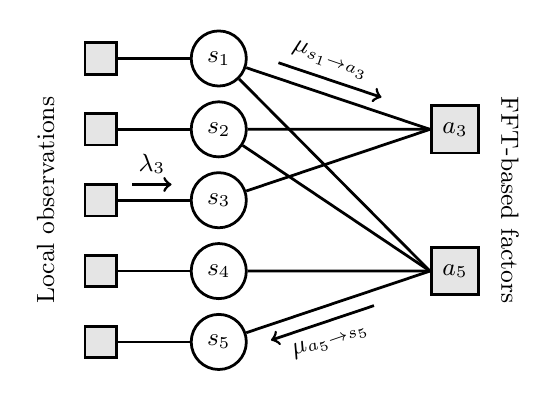
\begin{tikzpicture}
  [
  font=\small, line width=1pt, draw=black,
  check/.style={rectangle, minimum height=6mm, minimum width=6mm, draw=black, fill=gray!20},
  trivialcheck/.style={rectangle, minimum height=4mm, minimum width=4mm, draw=black, fill=gray!20},
  section/.style={circle, minimum size=7mm, draw=black}
  ]

\foreach \m in {1,2,3,4,5} {
  \node[section] (s\m) at (0,2.7-0.9*\m) {$s_{\m}$};
}

\foreach \t in {1,2,3,4,5} {
  \node[trivialcheck] (t\t) at (-1.5,2.7-0.9*\t) {}
    edge (s\t);
}

\node[check] (a3) at (3,0.9) {$a_3$};
\node[check] (a5) at (3,-0.9) {$a_5$};

\node[rotate=90] (variable) at (-2.2,0) {Local observations};
\node[rotate=-90] (check) at (3.7,0) {FFT-based factors};

\draw (s1) -- (a3.west);
\draw (s2) -- (a3.west);
\draw (s3) -- (a3.west);
\draw (s1) -- (a5.west);
\draw (s2) -- (a5.west);
\draw (s4) -- (a5.west);
\draw (s5) -- (a5.west);

\draw[shorten <=0.8cm,shorten >=0.65cm,->] (s1)++(0,0.2cm) -- node[above,rotate=-19] {$\muv_{s_1 \to a_3}$} ([yshift=0.2cm]a3.west);
\draw[shorten <=0.7cm,shorten >=0.75cm,<-] (s5)++(0,-0.2cm) -- node[below,rotate=19] {$\muv_{a_5 \to s_5}$} ([yshift=-0.2cm]a5.west);
\draw[shorten <=0.4cm,shorten >=0.4cm,->] (t3)++(0,0.2cm) -- node[above] {$\lambdav_3$} (-0.2,0.2cm);

\end{tikzpicture}
}
\end{center}
\begin{itemize}
\item Outer code with circular convolution structure
\end{itemize}
\begin{equation*}
\muv_{a_p \to s_{\ell}} \left( \left[ \hat{\vv}(\ell) \right]_2 \right)
\propto
\frac{1}{\left\| \gv_{\ell, p}^{(g)} \right\|_0}
\left( \operatorname{FFT}^{-1} \left( \prod_{s_j \in N(a_p) \setminus s_{\ell}} \operatorname{FFT} \left( \lambdav_{j,p} \right) \right) \right) (g)
\end{equation*}
\end{frame}

% % % % % % % % % % % % % % % % % % % %

\begin{frame}
\frametitle{Outer Code and Mixing}
% % % % %
\begin{center}
\scalebox{0.9}{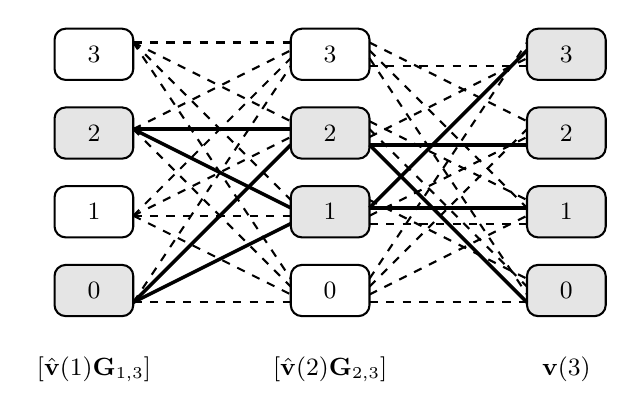
\begin{tikzpicture}[
  font=\small, >=stealth', line width=0.75pt,
  infobits/.style={rectangle, minimum height=6.5mm, minimum width=10mm, draw=black, fill=gray!20, rounded corners},
  paritybits/.style={rectangle, minimum height=6.5mm, minimum width=10mm, draw=black, fill=gray!20, rounded corners},
  impossibleblocks/.style={rectangle, minimum height=6.5mm, minimum width=10mm, draw=black, fill=none, rounded corners}
]

\node[infobits] (v10) at (0,0) {0};
\node[impossibleblocks] (v11) at (0,1) {{1}};
\node[infobits] (v12) at (0,2) {2};
\node[impossibleblocks] (v13) at (0,3) {{3}};

\node[impossibleblocks] (v20) at (3,0) {{0}};
\node[infobits] (v21) at (3,1) {1};
\node[infobits] (v22) at (3,2) {2};
\node[impossibleblocks] (v23) at (3,3) {{3}};

\node[paritybits] (v30) at (6,0) {{0}};
\node[paritybits] (v31) at (6,1) {{1}};
\node[paritybits] (v32) at (6,2) {2};
\node[paritybits] (v33) at (6,3) {3};

\foreach \y/\ya in {0/-0.15,1/-0.05,2/0.05,3/0.15}{
    \foreach \yb in {0,1,2,3}{
        \draw[dashed] (0.5,\y+\ya) -- (2.5,\yb+\ya);
    }
}

\foreach \yexit/\yentry in {0/0,1/1,2/2,3/3}{
    \draw[dashed] (3.5,\yexit-0.15) -- (5.5,\yentry-0.15);
}
\foreach \yexit/\yentry in {0/1,1/2,2/3,3/0}{
    \draw[dashed] (3.5,\yexit-0.05) -- (5.5,\yentry-0.05);
}
\foreach \yexit/\yentry in {0/2,1/3,2/0,3/1}{
    \draw[dashed] (3.5,\yexit+0.05) -- (5.5,\yentry+0.05);
}
\foreach \yexit/\yentry in {0/3,1/0,2/1,3/2}{
    \draw[dashed] (3.5,\yexit+0.15) -- (5.5,\yentry+0.15);
}

\draw[line width=1.25pt] (0.5,0-0.15) -- (2.5,1-0.15);
\draw[line width=1.25pt] (0.5,0-0.15) -- (2.5,2-0.15);
\draw[line width=1.25pt] (0.5,2+0.05) -- (2.5,1+0.05);
\draw[line width=1.25pt] (0.5,2+0.05) -- (2.5,2+0.05);

\draw[line width=1.25pt] (3.5,1+0.05) -- (5.5,1+0.05);
\draw[line width=1.25pt] (3.5,1+0.05) -- (5.5,3+0.05);
\draw[line width=1.25pt] (3.5,2-0.15) -- (5.5,2-0.15);
\draw[line width=1.25pt] (3.5,2-0.15) -- (5.5,0-0.15);


\node (w1) at (0,-1) {$\left[ \hat{\vv}(1) \mathbf{G}_{1,3} \right]$};
\node (w2) at (3,-1) {$\left[ \hat{\vv}(2) \mathbf{G}_{2,3} \right]$};
\node (p3) at (6,-1) {$\vv(3)$};

\end{tikzpicture}
}
\end{center}
\begin{itemize}
\item Multiple devices on same graph
\item Parity factor mix concentrated values
\item Suggests triadic outer structure
\end{itemize}
\end{frame}

% % % % % % % % % % % % % % % % % % % %

\begin{frame}
\frametitle{Redesigning Outer Code}
% % % % %
\begin{block}{Solutions to Integrate into AMP}
\begin{itemize}
\item Parity bits are generated over Abelian group amenable to\\
FWHT or FFT
\item Discrimination power proportional to \# parities
\end{itemize}
\end{block}
\begin{center}
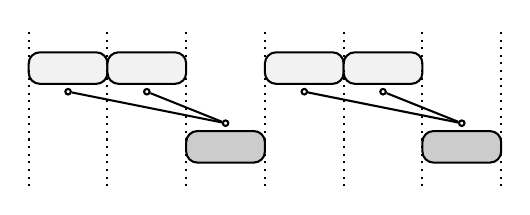
\begin{tikzpicture}[
  font=\footnotesize, >=stealth', line width=0.75pt,
  infobits/.style={rectangle, minimum height=4mm, minimum width=10mm, draw=black, fill=gray!10, rounded corners},
  paritybits/.style={rectangle, minimum height=4mm, minimum width=10mm, draw=black, fill=gray!40, rounded corners},
  dot/.style={circle, minimum width=2pt, draw=black, inner sep=0pt}
]

\node[infobits] (vb0) at (0,1) {};
\node[infobits] (vb1) at (1,1) {};
\node[paritybits] (vp2) at (2,0) {};
\node[infobits] (vb3) at (3,1) {};
\node[infobits] (vb4) at (4,1) {};
\node[paritybits] (vp5) at (5,0) {};

\node[dot] (vb0dot) at (0,0.7) {};
\node[dot] (vb1dot) at (1,0.7) {};
\node[dot] (vp2dot) at (2,0.3) {}
  edge[-] (vb0dot)
  edge[-] (vb1dot);
\node[dot] (vb3dot) at (3,0.7) {};
\node[dot] (vb4dot) at (4,0.7) {};
\node[dot] (vp5dot) at (5,0.3) {}
  edge[-] (vb3dot)
  edge[-] (vb4dot);

\foreach \x in {-0.5,0.5,1.5,2.5,3.5,4.5,5.5} {
    \draw[dotted] (\x,-0.5) -- (\x,1.5);
}
\end{tikzpicture}

\end{center}
\begin{block}{New Design Strategy}
\begin{enumerate}
\item Information sections with parity bits interspersed in-between
\item Parity over two blocks (triadic dependencies)
\end{enumerate}
\end{block}
\end{frame}

% % % % % % % % % % % % % % % % % % % %

\begin{frame}
\frametitle{Belief Propagation -- Message Passing Rules}
% % % % %
\begin{center}
\scalebox{0.85}{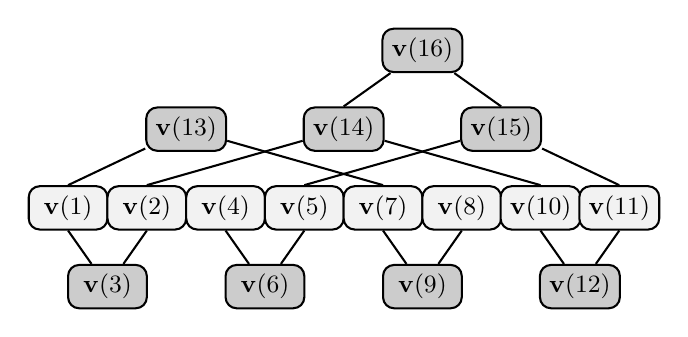
\begin{tikzpicture}[
  font=\small, >=stealth', line width=0.75pt,
  infobits/.style={rectangle, minimum height=3mm, minimum width=10mm, draw=black, fill=gray!10, rounded corners},
  paritybits/.style={rectangle, minimum height=3mm, minimum width=10mm, draw=black, fill=gray!40, rounded corners}
]

\node[infobits] (vb1) at (1,0) {$\mathbf{v}(1)$};
\node[infobits] (vb2) at (2,0) {$\mathbf{v}(2)$};
\node[infobits] (vb4) at (3,0) {$\mathbf{v}(4)$};
\node[infobits] (vb5) at (4,0) {$\mathbf{v}(5)$};
\node[infobits] (vb7) at (5,0) {$\mathbf{v}(7)$};
\node[infobits] (vb8) at (6,0) {$\mathbf{v}(8)$};
\node[infobits] (vb10) at (7,0) {$\mathbf{v}(10)$};
\node[infobits] (vb11) at (8,0) {$\mathbf{v}(11)$};

\node[paritybits] (vp3) at (1.5,-1) {$\mathbf{v}(3)$};
\node[paritybits] (vp6) at (3.5,-1) {$\mathbf{v}(6)$};
\node[paritybits] (vp9) at (5.5,-1) {$\mathbf{v}(9)$};
\node[paritybits] (vp12) at (7.5,-1) {$\mathbf{v}(12)$};
\node[paritybits] (vp13) at (2.5,1) {$\mathbf{v}(13)$};
\node[paritybits] (vp14) at (4.5,1) {$\mathbf{v}(14)$};
\node[paritybits] (vp15) at (6.5,1) {$\mathbf{v}(15)$};

\node[paritybits] (vp16) at (5.5,2) {$\mathbf{v}(16)$};

\draw  (vb1.south) edge (vp3);
\draw  (vb2.south) edge (vp3);
\draw  (vb4.south) edge (vp6);
\draw  (vb5.south) edge (vp6);
\draw  (vb7.south) edge (vp9);
\draw  (vb8.south) edge (vp9);
\draw  (vb10.south) edge (vp12);
\draw  (vb11.south) edge (vp12);

\draw  (vb1.north) edge (vp13);
\draw  (vb7.north) edge (vp13);
\draw  (vb2.north) edge (vp14);
\draw  (vb10.north) edge (vp14);
\draw  (vb5.north) edge (vp15);
\draw  (vb11.north) edge (vp15);
\draw  (vp14.north) edge (vp16);
\draw  (vp15.north) edge (vp16);

\end{tikzpicture}
}
\end{center}
\begin{itemize}
\item Message from check node $a_p$ to variable node $s \in N(a_p)$:
\begin{equation*}
\textstyle \muv_{a_p \to s} (k)
= \sum_{\kv_{a_p}: k_p = k} \mathcal{G}_{a_p} \left( \kv_{a_p} \right)
\prod_{s_j \in N(a_p) \setminus s} \muv_{s_j \to a_p} (k_j)
\end{equation*}
\item Message from variable node $s_{\ell}$ to check node $a \in N(s)$:
\begin{equation*}
\textstyle \muv_{s_{\ell} \rightarrow a} (k)
\propto \lambdav_{\ell} (k) \prod_{a_p \in N(s_{\ell}) \setminus a} \muv_{a_p \to s_{\ell}} (k)
\end{equation*}
\item Estimated marginal distribution
\begin{equation*}
\textstyle p_{s_{\ell}} (k) \propto \boldsymbol{\lambda}_{\ell} (k) \prod_{a \in N(s_{\ell})} \boldsymbol{\mu}_{a \to s_{\ell}} (k)
\end{equation*}
\end{itemize}
\end{frame}

% % % % % % % % % % % % % % % % % % % %

\begin{frame}
\frametitle{Approximate Message Passing Algorithm}
% % % % %
\begin{block}{Updated Equations}
AMP two-step algorithm
\begin{align*}
\zv^{(t)} &= \yv - \Am \Dm \etav_t \big( \rv^{(t)} \big)
+ \underbrace{\frac{\zv^{(t-1)}}{n} \operatorname{div} \mathbf{D} \etav_t \big( \rv^{(t)} \big)}_{\text{Correction}} \\
\rv^{(t+1)} &= \Am^{\transpose} \zv^{(t)} + \Dm
\underbrace{\etav_t \big( \rv^{(t)} \big)}_{\text{Denoiser}}
\end{align*}
\textcolor{gray}{Initial conditions $\zv^{(0)} = \zerov$ and $\etav_0 \left( \rv^{(0)} \right) = \zerov$}
\end{block}
\begin{itemize}
\item Denoiser is BP estimate from factor graph
\item Message passing uses fresh effective observation $\rv$
\item Fewer rounds than shortest cycle on factor graph
\item Close to PME, but incorporating beliefs from outer code
\end{itemize}
\myfootnote{\tiny
R. Berthier, A. Montanari, and P.-M. Nguyen.
\emph{State Evolution for Approximate Message Passing with Non-Separable Functions}.
Information and Inference: A Journal of the IMA 2020}
\end{frame}

% % % % % % % % % % % % % % % % % % % %

\begin{frame}
\frametitle{Preliminary Performance Enhanced CCS}
% % % % %
\centerline{
  \scalebox{0.65}{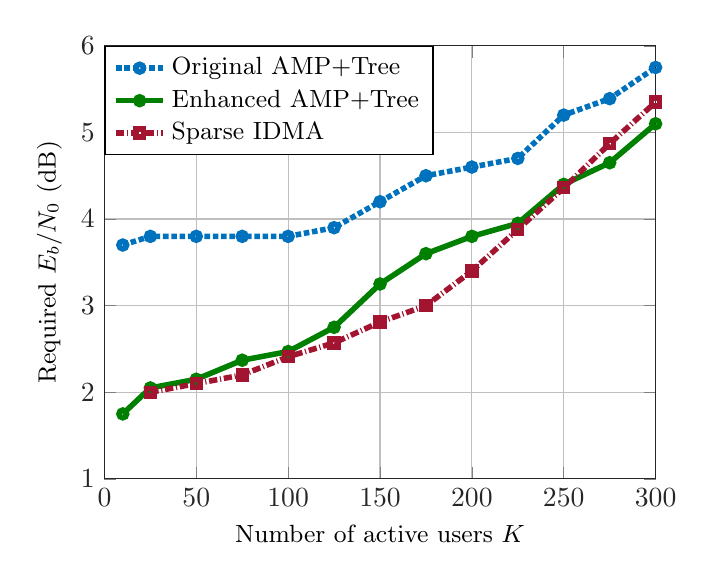
\begin{tikzpicture}
\definecolor{mycolor1}{rgb}{0.63529,0.07843,0.18431}%
\definecolor{mycolor2}{rgb}{0.00000,0.44706,0.74118}%
\definecolor{mycolor3}{rgb}{0.00000,0.49804,0.00000}%
\definecolor{mycolor4}{rgb}{0.87059,0.49020,0.00000}%
\definecolor{mycolor5}{rgb}{0.00000,0.44700,0.74100}%
\definecolor{mycolor6}{rgb}{0.74902,0.00000,0.74902}%

\begin{axis}[%
font=\small,
width=7cm,
height=5.5cm,
scale only axis,
every outer x axis line/.append style={white!15!black},
every x tick label/.append style={font=\color{white!15!black}},
xmin=0,
xmax=300,
xtick = {0,50,100,...,300},
xlabel={Number of active users $K$},
xmajorgrids,
every outer y axis line/.append style={white!15!black},
every y tick label/.append style={font=\color{white!15!black}},
ymin=1,
ymax=6,
ytick = {1,...,6},
ylabel={Required $E_b/N_0$ (dB)},
ymajorgrids,
legend style={at={(0,1)},anchor=north west, draw=black,fill=white,legend cell align=left}
]



\addplot [color=mycolor2,densely dotted,line width=2.0pt,mark size=1.4pt,mark=o, mark options={solid}]
  table[row sep=crcr]{10 3.7\\
25	3.8\\
50	3.8\\
75	3.8\\
100	3.8\\
125	3.9\\
150	4.2\\
175 4.5\\
200 4.6\\
225 4.7\\
250 5.2\\
275 5.39\\
300 5.75\\
};
\addlegendentry{Original AMP+Tree};

\addplot [color=mycolor3,solid,line width=2.0pt,mark size=1.4pt,mark=o,mark options={solid}]
  table[row sep=crcr]{10 1.75\\
  25  2.05\\
50	2.15\\
75	2.37\\
100	2.47\\
125	2.75\\
150	3.25\\
175 3.6\\
200 3.8\\
225 3.95\\
250 4.4\\
275 4.65\\
300 5.1\\
};
\addlegendentry{Enhanced AMP+Tree};

\addplot [color=mycolor1,densely dashdotted,line width=2.0pt,mark size=1.4pt,mark=square,mark options={solid}]
  table[row sep=crcr]{
  25  2\\
50	2.1\\
75	2.2\\
100	2.41\\
125	2.57\\
150	2.81\\
175	3\\
200 3.4\\
225 3.88\\
250 4.36\\
275 4.87\\
300 5.35\\
};
\addlegendentry{Sparse IDMA};


\end{axis}


\end{tikzpicture}
}
  \scalebox{0.65}{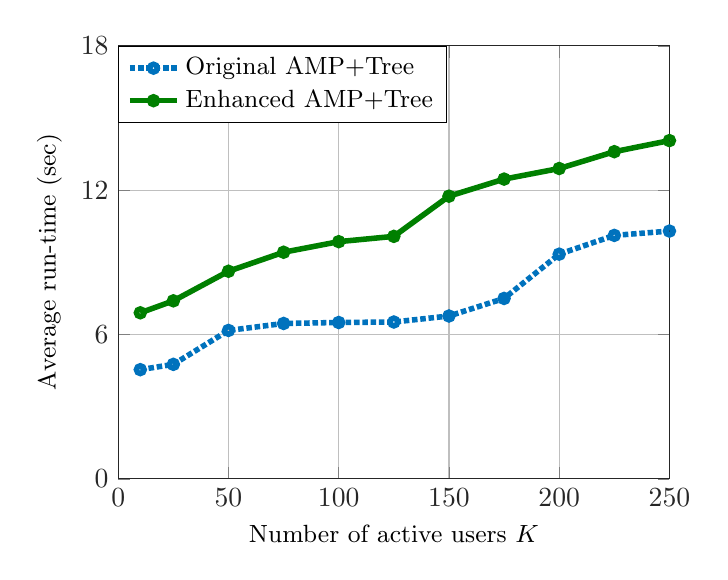
\begin{tikzpicture}
\definecolor{mycolor1}{rgb}{0.63529,0.07843,0.18431}%
\definecolor{mycolor2}{rgb}{0.00000,0.44706,0.74118}%
\definecolor{mycolor3}{rgb}{0.00000,0.49804,0.00000}%
\definecolor{mycolor4}{rgb}{0.87059,0.49020,0.00000}%
\definecolor{mycolor5}{rgb}{0.00000,0.44700,0.74100}%
\definecolor{mycolor6}{rgb}{0.74902,0.00000,0.74902}%

\begin{axis}[%
font=\small,
width=7cm,
height=5.5cm,
scale only axis,
every outer x axis line/.append style={white!15!black},
every x tick label/.append style={font=\color{white!15!black}},
xmin=0,
xmax=250,
xtick = {0,50,100,...,250},
xlabel={Number of active users $K$},
xmajorgrids,
every outer y axis line/.append style={white!15!black},
every y tick label/.append style={font=\color{white!15!black}},
ymin=0,
ymax=18,
ytick = {0,6,...,18},
ylabel={Average run-time (sec)},
ymajorgrids,
legend style={at={(0,1)},anchor=north west, draw=black,fill=white,legend cell align=left}
]



\addplot [color=mycolor2,densely dotted,line width=2.0pt,mark size=1.4pt,mark=o, mark options={solid}]
  table[row sep=crcr]{10 4.54\\
25	4.76\\
50	6.17\\
75	6.46\\
100	6.5\\
125	6.52\\
150	6.77\\
175 7.5\\
200 9.34\\
225 10.12\\
250 10.3\\
};
\addlegendentry{Original AMP+Tree};

\addplot [color=mycolor3,solid,line width=2.0pt,mark size=1.4pt,mark=o,mark options={solid}]
  table[row sep=crcr]{10 6.903\\
  25  7.4\\
50	8.63\\
75	9.42\\
100	9.86\\
125	10.08\\
150 11.75\\
175 12.46\\
200 12.9\\
225 13.6\\
250 14.06\\
};
\addlegendentry{Enhanced AMP+Tree};
\end{axis}

\end{tikzpicture}
}}
\vspace{5mm}
\begin{itemize}
\item Performance improves significantly with enhanced CCS-AMP decoding
\item Computational complexity is approximately maintained
\item Reparametrization may offer additional gains in performance?
\end{itemize}
\end{frame}

% % % % % % % % % % % % % % % % % % % %

\begin{frame}
\frametitle{CCS and AMP Summary}
% % % % %
\begin{block}{Summary}
\begin{itemize}
\item New connection between CCS and AMP
\item Natural application of BP on factor graph as denoiser
\item Outer code design depends on sparsity
\begin{enumerate}
\item Degree distributions (small graph)
\item Message size (birthday problem)
\item Final step is disambiguation
\end{enumerate}
\item Many theoretical and practical challenges/opportunities exist
\end{itemize}
\end{block}
\begin{center}
\scalebox{0.75}{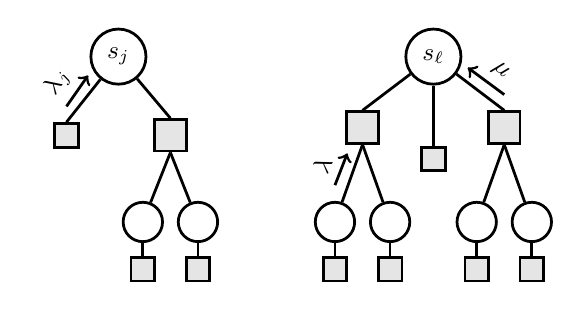
\begin{tikzpicture}
  [
  font=\small, line width=1pt, draw=black,
  check/.style={rectangle, minimum height=4mm, minimum width=4mm, draw=black, fill=gray!20},
  trivialcheck/.style={rectangle, minimum height=3mm, minimum width=3mm, draw=black, fill=gray!20},
  section/.style={circle, minimum size=7mm, draw=black},
  emptysection/.style={circle, minimum size=5mm, draw=black}
  ]

\node[section] (sp) at (0,0) {$s_{j}$};
\node[trivialcheck] (tp) at (-0.66,-1) {};
\node[check] (ap) at (0.66,-1) {};

\node[emptysection] (sp1) at (0.66-0.35,-0.9-1.2) {};
\node[trivialcheck] (tp1) at (0.66-0.35,-1.5-1.2) {}
    edge[-] (sp1);
\node[emptysection] (sp2) at (0.66+0.35,-0.9-1.2) {};
\node[trivialcheck] (tp2) at (0.66+0.35,-1.5-1.2) {}
    edge[-] (sp2);

\draw (sp) -- (tp.north);
\draw (sp) -- (ap.north);
\draw (sp1) -- (ap.south);
\draw (sp2) -- (ap.south);


\node[section] (sl) at (4,0) {$s_{\ell}$};
\node[trivialcheck] (tl) at (4,-1.3) {};
\node[check] (al1) at (4-0.9,-0.9) {};
\node[check] (al2) at (4+0.9,-0.9) {};

\node[emptysection] (sl11) at (3.1-0.35,-0.9-1.2) {};
\node[trivialcheck] (tl11) at (3.1-0.35,-1.5-1.2) {}
    edge[-] (sl11);
\node[emptysection] (sl12) at (3.1+0.35,-0.9-1.2) {};
\node[trivialcheck] (tl12) at (3.1+0.35,-1.5-1.2) {}
    edge[-] (sl12);

\node[emptysection] (sl21) at (4.9-0.35,-0.9-1.2) {};
\node[trivialcheck] (tl21) at (4.9-0.35,-1.5-1.2) {}
    edge[-] (sl21);
\node[emptysection] (sl22) at (4.9+0.35,-0.9-1.2) {};
\node[trivialcheck] (tl22) at (4.9+0.35,-1.5-1.2) {}
    edge[-] (sl22);

\draw (sl) -- (tl.north);
\draw (sl) -- (al1.north);
\draw (sl) -- (al2.north);
\draw (sl11) -- (al1.south);
\draw (sl12) -- (al1.south);
\draw (sl21) -- (al2.south);
\draw (sl22) -- (al2.south);


\draw[shorten <=0.22cm,<-] (sp.south west)++(0,0.2cm) -- node[above,rotate=58,xshift=-0.15cm] {$\lambdav_j$} ([yshift=0.2cm]tp.north);
\draw[shorten <=0.12cm,<-] (al1.south)++(-0.15cm,0) -- node[above,rotate=68,xshift=-0.1cm] {$\lambdav$} ([yshift=0.2cm]sl11.north);
\draw[shorten <=0.22cm,<-] (sl.south east)++(0,0.25cm) -- node[above,rotate=-45,xshift=0.15cm] {${\muv}$} ([yshift=0.2cm]al2.north);

\end{tikzpicture}
}
\end{center}
\centerline{Coding plays increasingly central role in large-scale CS}
\end{frame}

% % % % % % % % % % % % % % % % % % % %

\begin{frame}
\frametitle{Coded Demixing for Single-Class URA}
% % % % %
\begin{columns}
\column{0.52\textwidth}
  \centerline{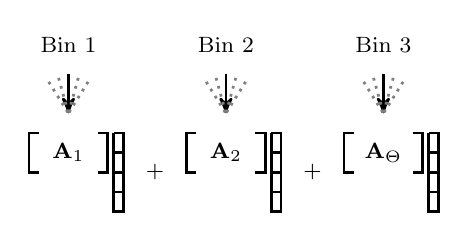
\begin{tikzpicture}
[font=\footnotesize, draw=black, line width=0.75pt,>=stealth',
sub0/.style={rectangle, draw, inner sep=0pt, minimum width=10mm, minimum height=2.5mm},
parity/.style={rectangle, draw, fill=teal, inner sep=0pt, minimum size=2.5mm}]

\node (cs1) at (0.00,6.125) {Bin~1};
\node (cs2) at (2.00,6.125) {Bin~2};
\node (cs3) at (4.00,6.125) {Bin~3};

\foreach \v in {0.00,2.00,4.00} {
  \draw[->, line width=1pt]  (\v,5.75) -- (\v,5.25);
  \draw[dotted, line width=1pt, draw=gray]  (\v-0.25,5.65) -- (\v,5.25);
  \draw[dotted, line width=1pt, draw=gray]  (\v-0.125,5.7) -- (\v,5.25);
  \draw[dotted, line width=1pt, draw=gray]  (\v+0.125,5.7) -- (\v,5.25);
  \draw[dotted, line width=1pt, draw=gray]  (\v+0.25,5.65) -- (\v,5.25);
}

\foreach \v in {0.00,2.00,4.00} {
  \draw[line width=1pt] (\v-0.375,5) -- (\v-0.5,5) -- (\v-0.5,4.5) -- (\v-0.375,4.5);
  \draw[line width=1pt] (\v+0.375,5) -- (\v+0.5,5) -- (\v+0.5,4.5) -- (\v+0.375,4.5);
  \draw[line width=1pt] (\v+0.575,5) -- (\v+0.575,4) -- (\v+0.7,4) -- (\v+0.7,5) -- (\v+0.575,5);
  \draw[line width=1pt] (\v+0.575,4.25) -- (\v+0.7,4.25);
  \draw[line width=1pt] (\v+0.575,4.5) -- (\v+0.7,4.5);
  \draw[line width=1pt] (\v+0.575,4.75) -- (\v+0.7,4.75);
}

\node at (0.00,4.75) {$\Am_1$};
\node at (2.00,4.75) {$\Am_2$};
\node at (4.00,4.75) {$\Am_{\Theta}$};

\node at (1.1, 4.5) {$+$};
\node at (3.1, 4.5) {$+$};
\end{tikzpicture}
}
  \begin{itemize}
  \item Create multiple bins with (incoherent) matrices
  \item Devices pick a bucket randomly and use CCS-AMP encoding
  \item Perform joint demixing CCS-AMP decoding at access point
  \end{itemize}
\column{0.46\textwidth}
  \centerline{\begin{tikzpicture}

\begin{semilogyaxis}[
font=\small,
width=4.4cm,
height=3.8cm,
scale only axis,
every x tick label/.append style={font=\scriptsize},
xmin=2.0,
xmax=3.4,
xtick={2.0, 2.2, 2.4, 2.6, 2.8, 3.0, 3.2, 3.4},
xlabel={$E_{b}/N_0$ (dB)},
xmajorgrids,
xminorgrids,
every y tick label/.append style={font=\scriptsize},
ymin=0.02,
ymax=1,
ytick={0.01, 0.1, 1.0},
%ylabel={Per-User Probability of Error $P_{\mathrm{e}}$},
ymajorgrids,
yminorgrids,
legend style={anchor=north east,draw=black, fill=white, legend cell align=left,font=\scriptsize, legend columns=2}
]

\addplot [color=black,line width=1.25pt,mark=x]
  table[row sep=crcr]{
  2.0 3.996874999999999734e-01\\
  2.2 3.126562500000000244e-01\\
  2.4 2.423437499999999967e-01\\
  2.6 1.876562499999999967e-01\\
  2.8 1.454687500000000078e-01\\
  3.0 1.110937500000000050e-01\\
  3.2 7.624999999999991507e-02\\
  3.4 5.203124999999998723e-02\\
};
\addlegendentry{$B=1$};

\addplot [color=blue,line width=1.25pt,mark=square,mark size=1.5pt,mark options={solid}]
  table[row sep=crcr]{
  2.0 3.168750000000000733e-01 \\
  2.2 0.24984375\\
  2.4 1.768750000000000322e-01 \\
  2.6 0.12390624999999997 \\
  2.8 8.203124999999994449e-02 \\
  % 3.0 4.749999999999996586e-02 \\
  3.0 0.05546016483516482 \\
  3.2 3.265625000000001860e-02 \\
};
\addlegendentry{$B=2$};

\addplot [color=purple,line width=1.25pt,mark=o,mark size=1.5pt,mark options={solid}]
  table[row sep=crcr]{
  2.0 2.570312500000000999e-01\\
  2.2 0.180665178563 \\
  2.4 1.135937499999999656e-01 \\
  2.6 7.078124999999996225e-02 \\
  2.8 4.796874999999996975e-02 \\
  3.0 2.875000000000002207e-02 \\
};
\addlegendentry{$B=4$};

\addplot [color=red,line width=1.25pt,mark=triangle,mark size=1.5pt,mark options={solid}]
  table[row sep=crcr]{
  2.0 1.824999999999999956e-01 \\
  2.2 1.288194444444443199e-01 \\
  2.4 8.234374999999996558e-02 \\
  2.6 5.093749999999998279e-02 \\
  2.8 3.265625000000001166e-02 \\
};
\addlegendentry{$B=8$};

\draw[black, line width=0.75pt] (axis cs:2,0.05) to (axis cs:3.4,0.05);
\node at (axis cs:2.3,0.044) {\scriptsize PUPE = 5\%};

\end{semilogyaxis}
\end{tikzpicture}
}
\end{columns}
\myfootnote{\tiny
J.~R. Ebert, V.~K. Amalladinne, S. Rini, J.-F. Chamberland, K.~R. Narayanan.
\emph{Stochastic Binning and Coded Demixing for Unsourced Random Access.}
arXiv:2104.05686}
\end{frame}

% % % % % % % % % % % % % % % % % % % %

\begin{frame}
\frametitle{Pertinent References}
\begin{scriptsize}
\begin{itemize}
\item
A.~Fengler, P.~Jung, and G.~Caire.
SPARCs and AMP for Unsourced Random Access.
In \emph{International Symposium on Information Theory (ISIT)}, 2019.

\item
V.~K. Amalladinne, A.~K. Pradhan, C. Rush, J.-F. Chamberland, K.~R. Narayanan.
On approximate message passing for unsourced access with coded compressed sensing.
In \emph{International Symposium on Information Theory (ISIT)}, 2020.

\item
V.~K. Amalladinne, A. Hao, S. Rini, J.-F. Chamberland.
Multi-Class Unsourced Random Access via Coded Demixing.
In \emph{International Symposium on Information Theory (ISIT)}, 2021.

\item
A. Joseph, and A. R. Barron.
Least squares superposition codes of moderate dictionary size are reliable at rates up to capacity
\emph{IEEE Trans.\ on Information Theory}, 2012.

\item
C. Rush, A. Greig, and R. Venkataramanan.
Capacity-achieving sparse superposition codes via approximate message passing decoding.
\emph{IEEE Trans.\ on Information Theory}, 2017.

\item
R. Berthier, A. Montanari, and P.-M. Nguyen.
State Evolution for Approximate Message Passing with Non-Separable Functions.
\emph{Information and Inference: A Journal of the IMA}, 2020.
\end{itemize}
\end{scriptsize}
\end{frame}

% % % % % % % % % % % % % % % % % % % %


\end{document}

